\chapter{Eksperimenti}\label{sec:eksperimenti}
V tem poglavju predstavljamo eksperimente, ki smo jih izvedli v dveh različnih okoljih: v fiziološkem laboratoriju in na squash igrišču (terenski testi). Z njimi smo naslovili energijsko porabo $eem(t)$ kot osrednji fiziološki parameter. Srčni utrip $hr(t)$ smo obravnavali kot sekundarni parameter, z razumevanjem, da slabo odraža dejansko energijsko porabo. Z eksperimenti detekcije dihanja smo želeli preizkusiti predlagano metodo za širšo uporabo.

Pri vseh naslovljenih fizioloških parametrih smo s pomočjo strojnega učenja izvajali predikcijo časovnih signalov $eem(t)$ za energijsko porabo, $hr(t)$ za srčni utrip in $dihanje(t)$ za dihanje. Predikcijo smo izvajali iz posamezne slike zaporedja video posnetka. Pri tem smo najprej generirali sliko optičnega ali prostorskega toka in nato določili področje, kjer se nahaja merjenec. Iz izbranega področja smo izračunali vektorje značilk $\vec{x}(t)$, te pa smo uporabili za predikcijo. Rezultat je zelo enostaven, skoraj realno-časoven model, ki ga lahko razširimo s časovnim modeliranjem, če bi se pojavila potreba. 

Prvi del postopka je učenje SVM/SVR modela, kot je prikazano na sliki~\ref{fig:shema-generalnega-postopka01}. Na ta način dobimo parametre regresijskega modela, ki jih nato uporabimo za napovedovanje porabe energije iz testnih podatkov, kot je prikazano na sliki~\ref{fig:shema-generalnega-postopka02}.

\begin{figure}[!htb]
	\centering
	\resizebox{\columnwidth}{!}{\begin{tikzpicture}
% LAYERS
\pgfdeclarelayer{bg}
\pgfsetlayers{bg,main}
\tikzset{
	between/.style args={#1 and #2}{
		at = ($(#1)!0.5!(#2)$)
	}
}

% NODES
\node (slika) [input] at (0,0) {Področje tarče\\na sliki $I(x,y)$};

\node (of) [block, right= of slika] {Optični/Prostorski\\tok};
\node (hoof) [block, right= of of] {deskriptorji\\$\vec{x}(t)$};


\node (ucenje) [block, right=of hoof] {Postopek učenja};

\node (rezultat) [output, right= of ucenje] {SVM/SVR\\parametri};

% arrows
\draw [arrow] (slika) -- (of);


\draw [arrow] (of) -- (hoof);
\draw [arrow] (hoof) -- (ucenje);

\draw [arrow] (ucenje) -- (rezultat);
\end{tikzpicture}}
	\caption[Shema generalnega postopka učenja]{Shema generalnega postopka učenja. Iz izbranega področja tarče generiramo sliko toka in izračunamo vektorje značilk $\vec{x}(t)$. Te nato uporabimo za učenje realno-časovnih modelov, s katerimi izvajamo predikcijo fizioloških parametrov.}
	\label{fig:shema-generalnega-postopka01}
\end{figure}

\begin{figure}[!htb]
	\centering
	\resizebox{\columnwidth}{!}{\begin{tikzpicture}
% LAYERS
\pgfdeclarelayer{bg}
\pgfsetlayers{bg,main}
\tikzset{
	between/.style args={#1 and #2}{
		at = ($(#1)!0.5!(#2)$)
	}
}

% NODES
\node (slika) [input] at (0,0) {Področje tarče\\na sliki $I(x,y)$};

\node (of) [block, right= of slika] {Optični/Prostorski\\tok};
\node (hoof) [block, right= of of] {Deskriptorji\\$\vec{x}(t)$};

\node (params) [input, above=of hoof] {SVM/SVR\\parametri};
\node (ucenje) [block, right=of hoof] {Predikcija (testiranje)};

\node (rezultat) [output, right= of ucenje] {Energijska poraba};

% arrows
\draw [arrow] (slika) -- (of);


\draw [arrow] (of) -- (hoof);
\draw [arrow] (hoof) -- (ucenje);
\draw [arrow,] (params) to[out=0,in=90] (ucenje);

\draw [arrow] (ucenje) -- (rezultat);
\end{tikzpicture}}
	\caption[Shema generalnega postopka predikcije]{Shema generalnega postopka predikcije. Vhodni podatki so testni podatki.}
	\label{fig:shema-generalnega-postopka02}
\end{figure}

Eksperimente smo kronološko razdelili na dve fazi. V \emph{1. fazi} smo analizirali observabilnost izbranih fizioloških parametrov. Parameter je observabilen, če obstaja neničelna (pozitivna) korelacija med našo oceno parametra iz značilk gibanja in merjenih vrednosti, ki smo jih dobili iz zanesljivih metod pridobivanja fizioloških parametrov. %V 1. fazi smo posebej naslovili preliminarne teste, laboratorijske eksperimente tekalne steze, terenske eksperimente squash igre ter eksperimente dihanja. V {preliminarnih testih} opisujemo teste, s katerimi smo določili optimalne vrednosti parametrov. 
V \emph{eksperimentih 2. faze} smo optimizirali posamezne dele ocenjevanja fizioloških parametrov. %Sledi končna preiskava. Končna preiskava je sestavljena iz preliminarnih testov, laboratorijske in terenske preiskave. V preliminarnih testih smo optimizirali dele postopka, s katerim smo v 1. fazi eksperimentov dobili najboljše rezultate. V laboratorijskih in terenskih preiskavah smo uporabili tri različne protokole.

\renewcommand{\folder}{./pogl/03-eksperimenti}
\section{Eksperimenti 1. faze}
\subsection{Preliminarni testi}
\subsubsection{Optimizacija HOOF deskriptorjev}\label{sec:optimizacija-hoof}
Parameter $N_{HOOF}$ smo določili na podlagi rezultatov iz poglavja \ref{sec:rezultati-optimizacija-hoof}. Za evaluacijo smo uporabili učne vzorce hrbtne kamere preliminarnih laboratorijskih testov. Evaluirali smo samo za podatke energijske porabe $W$. Pridobljene značilke deskriptorjev smo normirali na intervalu $[-1,1]$ in jih uporabili za učenje regresijskega modela z metodo podpornih vektorjev $\epsilon$-SVR in jedrom RBF. Metode so podrobneje predstavljene v poglavju \ref{sec:matematicni-modeli}. Za določitev optimalnih parametrov, ki so predstavljeni v tabeli \ref{tab:nhoof-param}, smo uporabili optimizacijsko metodo mrežnega iskanja \cite{hsu2003practical}. Rezultate smo filtrirali še s Kalmanovim filtrom, ki je predstavljen v \ref{sec:kalmanov-filter}.

\begin{table}[htb]
	\centering
	\begin{tabular}{S[table-format=2.0] S[table-format=2.3] S[table-format=1.3] S[table-format=1.3] S[table-format=1.3]}
		\toprule
		\thead{$\mathbf{N_{HOOF}}$} & \thead{$\mathbf{C}$} & \thead{$\mathbf{\gamma}$} & \thead{$\mathbf{\epsilon}$} & \thead{MSE} \\ 
		\midrule
		30 & 8 & 0.707 & 0.812 & 7.903 \\
		60 & 8 & 0.354 & 0.379 & 7.320 \\
		120 & 11.314 & 0.177 & 0.536 & 6.998 \\
		160 & 11.314 & 0.125 & 0.616 & 6.832 \\
		\bottomrule
	\end{tabular}
	\caption[Optimalni parameteri RBF jedra modelov za določitev $N_{HOOF}$]{Optimalni parametri RBF jedra za modele z različnim številom stolpcev $N_{HOOF}$ v HOOF deskriptorju. Z njimi smo učili modele s katerimi smo preverjali optimalno število stolpcev v HOOF deskriptorju}
	\label{tab:nhoof-param}
\end{table}







\subsubsection{Optimizacija HAFA deskriptorjev}
Parameter $N_{HAFA}$ smo določili na podlagi rezultatov \ref{sec:rezultati-optimizacija-hafa}. Za evaluacijo smo uporabili enak eksperimentalni protokol kot za HOOF značilke v poglavju \ref{sec:hoof}, s to razliko, da smo značilke normirali na intervalu $[0, 1]$ in odstranili stolpec z amplitudami $0.5$. S tem smo odstranili šum, ki se je pojavil, ko ni bilo nobenega gibanja. Amplitudo šuma smo določili, kot maksimalno vrednost amplitude, ki še ni predstavljala gibanja. Optimalni parametri evaluacijske metode so predstavljeni v tabeli \ref{tab:nhafa-param}.


\begin{table}[!htb]
	\centering
	\begin{tabular}{S[table-format=2.0] S[table-format=2.3] S[table-format=1.3]  S[table-format=1.3] S[table-format=1.3]}
		\toprule
		\thead{$\mathbf{N_{HAFA}}$} & \thead{$\mathbf{C}$} & \thead{$\mathbf{\gamma}$} & \thead{$\mathbf{\epsilon}$} & \thead{MSE} \\ 
		\midrule
		30 & 8 & 5.657 & 0.616 & 4.329 \\
		60 & 8 & 5.657 & 0.616 & 4.327 \\
		120 & 8 & 5.657 & 0.616 & 4.327 \\
		160 & 8 & 5.657 & 0.616 & 4.327 \\
		\bottomrule
	\end{tabular}
	\caption[Optimalni parameteri RBF jedra modelov za določitev $N_{HAFA}$]{Optimalni parametri RBF jedra za modele z različnim številom stolpcev $N_{HAFA}$ v HAFA deskriptorju. Z njimi smo učili modele s katerimi smo preverjali optimalno število stolpcev v HAFA deskriptorju.}
	\label{tab:nhafa-param}
\end{table}






\subsubsection{Razširitev HOOF deskriptorja}\label{sec:razsiritev-hoof-rezultati}
HOOF deskriptorju smo pripeli HAFA deskriptor in tako dobili razširjeni deskriptor HOOF-HAFA, ki po evaluaciji iz poglavja \ref{sec:rezultati-razsiritev-hoof} v splošnem daje boljše rezultate.

Pri evaluaciji deskriptorjev HOOF in HOOF-HAFA smo uporabili učne vzorce hrbtne kamere terenskih testov. Evaluirali smo za podatke srčnega utripa $hr$. Srčni utrip smo za gradnjo modelov pretvorili v energijsko porabo $W$ po enačbi \eqref{eq:charlot}. Pridobljene značilke smo normirali na intervalu [0,1] in jih uporabili za učenje regresijskega modela z metodo podpornih vektorjev $\epsilon$-SVR in jedrom RBF. Za določitev optimalnih parametrov, ki so predstavljeni v tabeli \ref{tab:nhoof-param}, smo uporabili optimizacijsko metodo mrežnega iskanja \cite{hsu2003practical}. Rezultate smo filtrirali še s Gaussovim jedrom (predstavljen v \ref{sec:gaussov-filter}) velikosti $6$ in varianco $\sigma=16$. 

\begin{table}[htb]
	\centering
	\begin{tabular}{l S[table-format=2.3] S[table-format=1.3] S[table-format=1.3] S[table-format=1.3]}
		\toprule
		\textbf{Deskriptor} & \thead{$\mathbf{C}$} & \thead{$\mathbf{\gamma}$} & \thead{$\mathbf{\epsilon}$} & \thead{MSE} \\ 
		\midrule
		HOOF & 2.828 & 11.314 & 0.435 & 2.192 \\
		HOOF-HAFA & 5.657 & 2.828 & 0.154 & 1.781 \\
		\bottomrule
	\end{tabular}
	\caption[Optimalni parameteri RBF jedra modelov za izbiro deskriptorjev]{Optimalni parametri RBF jedra za modele z različnim deskriptorjem. Z modeloma smo preverjali razširitev HOOF deskriptorja v HOOF-HAFA deskriptor.}
	\label{tab:izbira-param}
\end{table}














\subsubsection{Testiranje sledilnikov za optični tok}\label{sec:testiranje-sledilnikov-za-opticni-tok}
Sledilnike smo testirali na sekvencah slik \textit{handball1} in \textit{handball2} podatkovne baze VOT2016 \cite{kristan2016visual}.Primer posnetkov je viden na sliki \ref{fig:testiranje-tracker-visual}. Sledila je še hitra vizualna ocena delovanja na kratkih izsekih video posnetka \cite{squashtv2014squash}. Primer posnetka je viden na sliki \ref{fig:testiranje-squash-1-kcf}.

\begin{figure}[!htbp]
	\centering
	
	\begin{subfigure}[t]{0.45\columnwidth}
		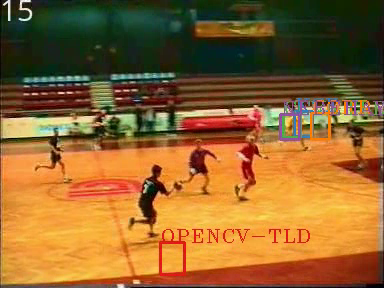
\includegraphics[width=\columnwidth]{handball1-example.png}
		\caption{15. slika posnetka \textit{handball1}.}
		\label{fig:testiranje-handball1}
	\end{subfigure}
	~
	\begin{subfigure}[t]{0.45\columnwidth}
		\includegraphics[width=\columnwidth]{handball2-example.png}
		\caption{111. slika posnetka \textit{handball2}.}
		\label{fig:testiranje-handball2}
	\end{subfigure}  
	\caption[Primer delovanja sledilnikov za \textit{handball} posnetke]{Primer delovanja sledilnikov za \textit{handball} posnetke. Referenčni igralec, ki mu morajo slediti ima rumeno majico. }
	\label{fig:testiranje-tracker-visual}
\end{figure}



\begin{figure}[htbp]
	\centering
	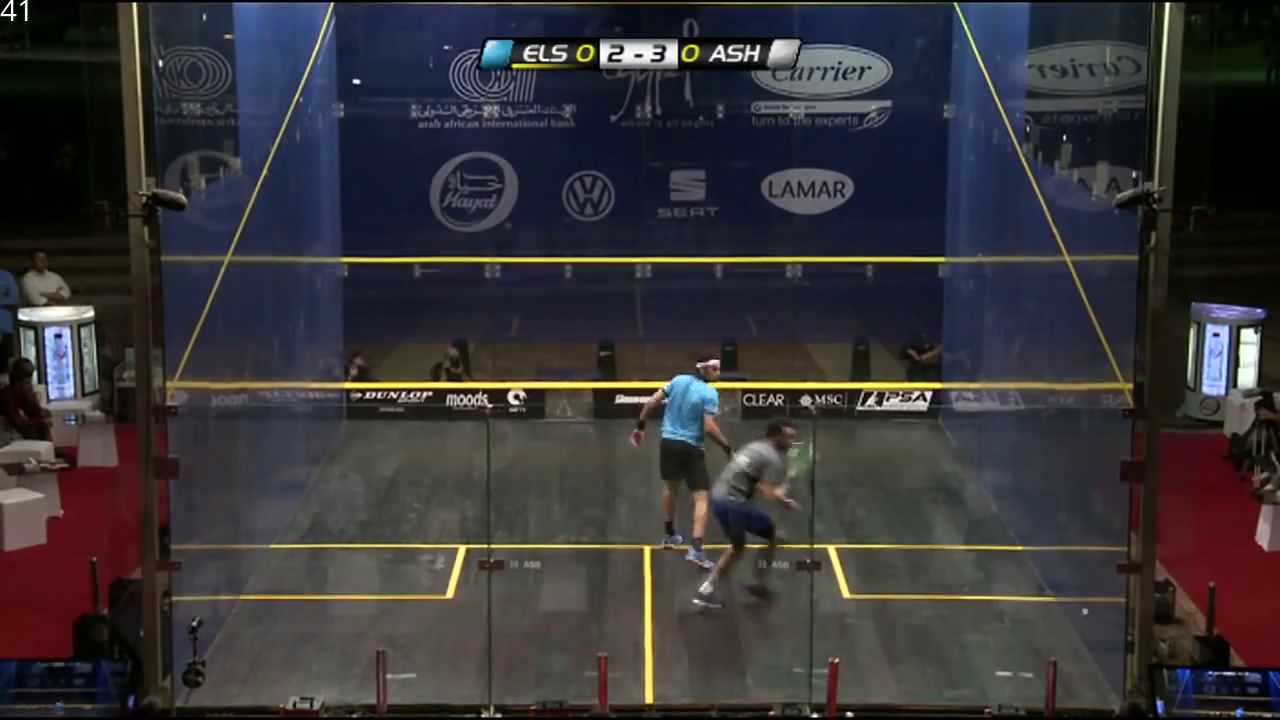
\includegraphics[width=0.6\columnwidth]{preliminary-squash-no-tracker.png}
	\caption[Uporaba squash posnetka za vizualno oceno delovanja sledilnikov]{Uporaba squash posnetka za vizualno oceno delovanja sledilnikov. Predstavljena je 41. slika posnetka \cite{squashtv2014squash}, kjer smo preizkušali KCF sledilnik. Sledili smo igralcu v svetlo modri majici. Modri okvir prikazuje področje, ki ga je sledilnik zaznal.}
	\label{fig:testiranje-squash-1-kcf}
\end{figure}



Pri testiranju sekvenc slik podatkovne baze VOT2016 smo poenostavili rotirajoča referenčna področja detekcij na nerotirajoča področja. Pri tem smo za zgornji levi kot $T_0(x,y)$ in spodnji desni kot $T_1(x,y)$ uporabili enačbo \eqref{eq:vot-bb}, kjer so $\left( x_i, y_i\right), \forall i=1,\ldots,4$ ogljišča rotirajočega referenčnega področja. 

\begin{equation}
\begin{aligned}
T_0(x,y) &= \left( \min_{i = 1,\ldots,4}\left\{x_i \right\}, 
\min_{i=1,\ldots,4}\{y_i \} \right) \\
T_1(x,y) &= \left( \max_{i = 1,\ldots,4}\left\{x_i \right\}, 
\max_{i=1,\ldots,4}\{y_i \} \right)
\end{aligned}
\label{eq:vot-bb}
\end{equation}

Ker je za naš sledilnik najbolj pomembno zanesljivo delovanje, smo izbrali mero prekrivanja področja.


Video posnetek \cite{squashtv2014squash} smo za potrebe vizualne ocene delovanja na squash posnetkih razdelili na več kratkih izsekov. Pri tem smo uporabili le hrbtne posnetke mirujoče kamere. 







\subsection{Laboratorijski eksperimenti tekalne steze}
Prve eksperimente smo izvedli v laboratoriju za fiziologijo na Fakulteti za šport. Merjenec je tekel na tekalni stezi ob prisotnosti operaterja---zdravnika, ki je določal intenziteto in čas trajanja obremenitve. Pri tem smo merili srčni utrip in enrgijsko porabo športnika (starost: 26 let, višina: \SI{177}{\cm}, teža: \SI{79.1}{\kg}, $VO_2max$: \SI{3705}{\ml\per\min}). Energijsko porabo smo merili z indirektno kalorimetrijo, in sicer s ``breath by breath'' Cosmed CPET Metabolic Cart \cite{beaver1973line}. Pri tem smo uporabili Hans Rudolph obrazno masko s predpisanim minimalnim VD (mrtvim prostorom).


\subsubsection{Pridobivanje podatkov}
Tekalno stezo smo snemali iz dveh različnih zornih kotov: hrbtni del in stranski del. Zaradi časovne neusklajenosti posnetkov smo jih sinhronizirali glede na začetno sliko meritev. Zaradi rahlo različne časovne frekvence na posameznih kamerah, se časovne neusklajenosti do potankosti nismo mogli znebiti. Ta se je akumulirala skozi čas. Pridobili smo posnetke barvnih RGB slik in infrardeče IR posnetke hrbtnega dela. Primer hrbtnega stranskega  in IR posnetka je prikazan na sliki \ref{fig:primer-posnetka-rgb-ir}.

\begin{figure}[htb]
	\centering
	\begin{subfigure}[t]{0.3\columnwidth}
		\centering
		\includegraphics[width=\columnwidth]{normal-sv-150.png}
		\caption{Stranska RBG slika.}
	\end{subfigure}
	~
	\begin{subfigure}[t]{0.3\columnwidth}
		\centering
		\includegraphics[width=\columnwidth]{normal-bv-150.png}
		\caption{Hrbtna RGB slika.}
	\end{subfigure}
	~
    \begin{subfigure}[t]{0.3\columnwidth}
    	\centering
		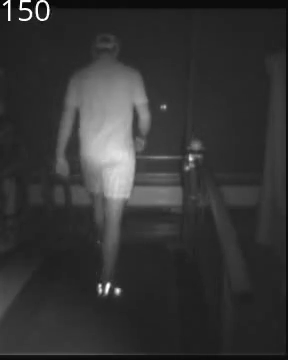
\includegraphics[width=0.6\columnwidth]{normal-ir-150.png}
		\caption{Hrbtna IR slika.}
	\end{subfigure}
	\caption[Hrbtna, stranska in IR 150. slika posnetkov iz prve serije]{Hrbtna, stranska in IR 150. slika posnetkov iz prve serije. Kljub časovni sinhronizaciji med posnetkoma, se časovni neusklajenosti nismo mogli popolnoma izogniti. Časovni frekvenci kamer nista bili sinhronizirani.}
	\label{fig:primer-posnetka-rgb-ir}
\end{figure}

Snemali smo v ločljivosti $480 \times 640$. Hitrost RGB posnetkov je bila \SI{30}{fps}, za IR posnetke pa je hitrost znašala \SI{25}{fps}.  Naklon tekalne steze je bil od \SI{1.5}{\%} do \SI{2}{\%}.



\subsubsection{Protokoli izvajanja meritev}
Naredili smo dve seriji testov v razmiku 20 minut. Fiziološke parametre smo vzorčili vsakih \SI{5}{\s}. V prvi seriji smo naredili 8 testov, kjer so vsi trajali 2 minuti. Hitrost tekalne steze smo vsak test povečali za \SI{1}{\km\per\hour}. Prvi test je imel hitrost  \SI{6}{\km\per\hour} zadnji pa \SI{13}{\km\per\hour}.

V drugi seriji smo naredili 3 teste po 5 minut. Hitrosti tekalne steze so bile  \SI{7}{\km\per\hour}, \SI{10}{\km\per\hour} in \SI{13}{\km\per\hour}.

Prvo serijo testov smo uporabili za pridobitev učnih vzorcev. Drugo serijo smo uporabili za testne vzorce.


\subsubsection{Elementarni postopek procesiranja}\label{sec:elementarni-postopek}
Kot smo že omenili so bile meritve fizioloških parametrov izvedene z vzorčenjem \SI{5}{\s} oziroma s frekvenco \SI{0.2}{\hertz}. Hitrost posnetkov je bila \SI{30}{fps} za RGB in \SI{25}{fps} za IR slike. Zaradi neskladja frekvenc vzorčenja slik in fizioloških parametrov, smo te interpolirali s pomočjo Matlabove funkcije \texttt{interp1}.
 
Za izbrano področje slike iz zaporedja posameznega posnetka smo nato izračunali optični tok. Primer dobljenega optičnega toka je prikazan na sliki \ref{fig:opticni-tok-stage1} Enote optičnega toka so \si{ppf}. Pomenijo število slikovnih elementov na sliko (ang. Pixel per Frame).


\begin{figure}[!htb]
	\centering
	\begin{subfigure}{0.45\columnwidth}
		\includegraphics[width=\columnwidth]{./Slike/normal-sv-150.png}
		\caption{Originalna slika.}
	\end{subfigure}
	~
	\begin{subfigure}{0.45\columnwidth}
	    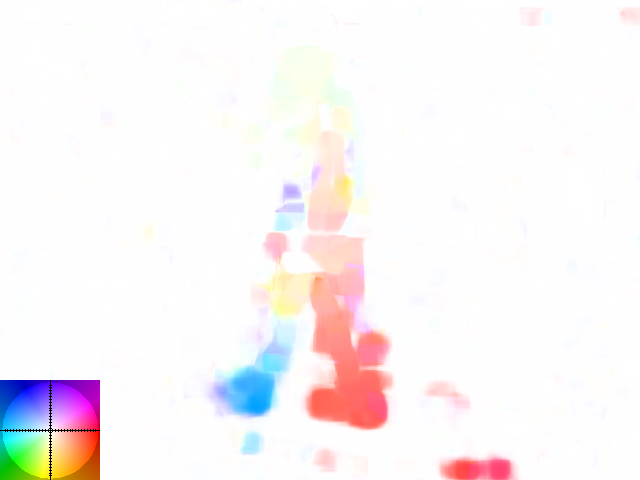
\includegraphics[width=\columnwidth, frame]{./Slike/normal-sv-of-coded-150.png}
		\caption{Slika optičnega toka.}
		\label{fig:stage1-of}
	\end{subfigure}
    \caption[Originalna $150$. stranska slika in optični tok]{Originalna $150$. stranska slika in njen optični tok. Gre za sliko 1. serije testov. Na sliki \subref{fig:stage1-of} je legenda barvnega kodiranja v spodnjem levem kotu s standardnim barvnim kodiranjem, ki je povzeto po \cite{baker2011database}. Maksimalna amplituda optičnega toka je na tej sliki znašala \SI{17}{ppf}.}
    \label{fig:opticni-tok-stage1}
\end{figure}

Sledilo je generiranje HOOF deskriptorjev, ki smo jih pred tem optimizirali po postopku, opisanem v poglavju \ref{sec:optimizacija-hoof}. Za parameter smo izbrali $N_{HOOF} = 60 $, ker je dal najbolj optimalne rezultate. Primer HOOF deskriptorjev lahko vidimo na sliki \ref{fig:hoof-znacilke}.

\begin{figure}[!htb]
	\centering
	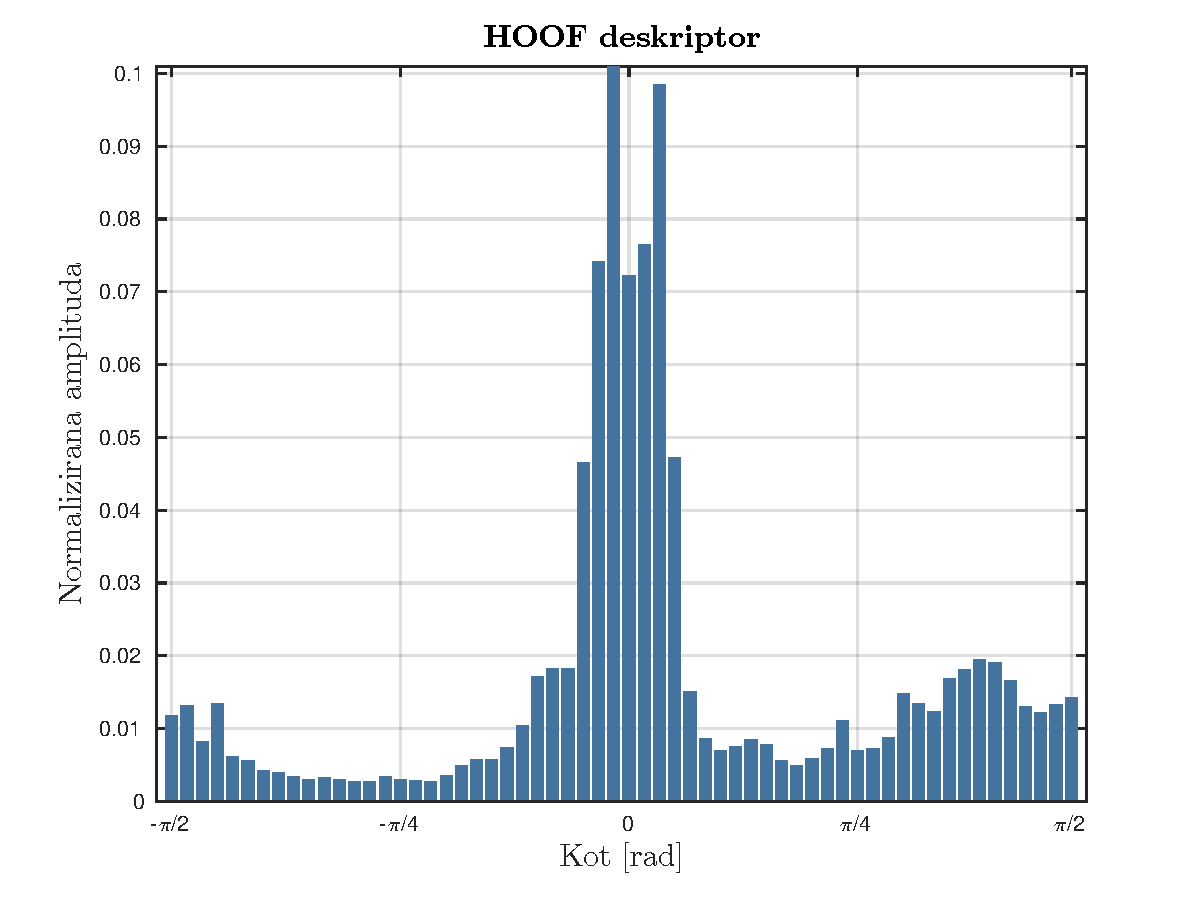
\includegraphics[width=0.75\columnwidth]{stage1-lab-sv-hist-sl}
	\caption[HOOF deskriptor za 150. RGB sliko prve serije]{HOOF deskriptor za 150. RGB sliko prve serije. Deskriptor smo izračunali iz slike \ref{fig:opticni-tok-stage1}.}
	\label{fig:hoof-znacilke}
\end{figure}

Modele smo učili z metodo podpornih vektorjev $\epsilon$-SVR in jedrom RBF. Regresijske parametre jedra smo optimizirali z metodo mrežnega iskanja. Naučili smo \num{8} elementarnih modelov, ki smo jih razdelili na dve kategoriji: na \textit{hr} modele, ki predvidevajo srčni utrip in modele \textit{eem}, ki predvidevajo porabo energije v \si{\kcal\per\min}. Kategoriji sta nadalje razdeljeni glede na zorni kot kamere: \textit{sv} modeli za stransko kamero in \textit{bv} modeli za hrbtno kamero. Eksperimente smo razširili z vpeljavo zakasnitve med referenčnim fiziološkim parametrom in merjenim parametrom iz slik posnetka. Z eksperimenti, ki so označeni z \textit{lag} kratico, smo preverili predlagano časovno zakasnitev med vzbujanjem in fiziološkim odzivom. 

Generirali smo tudi dodatne modele, in sicer: \textit{crop} modele, \textit{mixed} modele, \textit{track} modele, kjer smo uporabili sledilnik in obremenitvene modele. Ti so deljeni na \textit{scale} modele in \textit{proj} modele.

Vse tipe eksperimentov smo križno testirali glede na enak tip eksperimenta, le z drugim zornim kotom kamere. Uporabljen zorni kot kamere za križno testiranje je v imenih modelov zapisan v oklepajih. Rezultate smo pred testiranjem filtrirali s Kalmanovim filtrom. Uporabljeni parametri so opisani v poglavju \ref{sec:implementacija-kalman}.


\begin{figure}[!htb]
	\centering
	\resizebox{\columnwidth}{!}{\begin{tikzpicture}
% LAYERS
\pgfdeclarelayer{bg}
\pgfsetlayers{bg,main}
\tikzset{
    between/.style args={#1 and #2}{
         at = ($(#1)!0.5!(#2)$)
    }
}

% NODES
\node (slika) [input] at (0,0) {Področje\\slike $I(x,y)$};

\node (of) [block, right= of slika] {Optični\\ tok $\vec{w}$};
\node (hoof) [block, right= of of] {HOOF\\deskriptor $\vec{x}(t)$};


\node (ucenje) [block, right=of hoof] {$\epsilon$-SVR\\RBF jedro};
\node (kalman) [block, right= of ucenje] {Kalmanov\\filter};


\node (rezultat) [output, right= of kalman] {Rezultat};

% arrows
\draw [arrow] (slika) -- (of);
\draw [arrow] (of) -- (hoof);
\draw [arrow] (hoof) -- (ucenje);
\draw [arrow] (ucenje) -- (kalman);
\draw [arrow] (kalman) -- (rezultat);
\end{tikzpicture}}
	\caption[Diagram postopka za eksperimente 1. faze]{Diagram postopka za eksperimente 1. faze. Izbranemu področju na sliki določimo optični tok.}
	\label{fig:diagram-procesiranja-stage1}
\end{figure}

\subsubsection{Določitev dodatne zakasnitve}
Na podlagi slike \ref{fig:lag-estimation-stage1} smo določili dodatno zakasnitev spremembe hitrosti tekalne steze. Z vpeljavo zakasnitve smo želeli preveriti pravilnost sinhronizacije merjenih podatkov in kamere. Celoten odziv posameznega fiziološkega parametra je prikazan na sliki \ref{fig:odziv-stage1}.


\begin{figure}[!htb]
	\centering
	\begin{subfigure}[t]{0.45\columnwidth}
		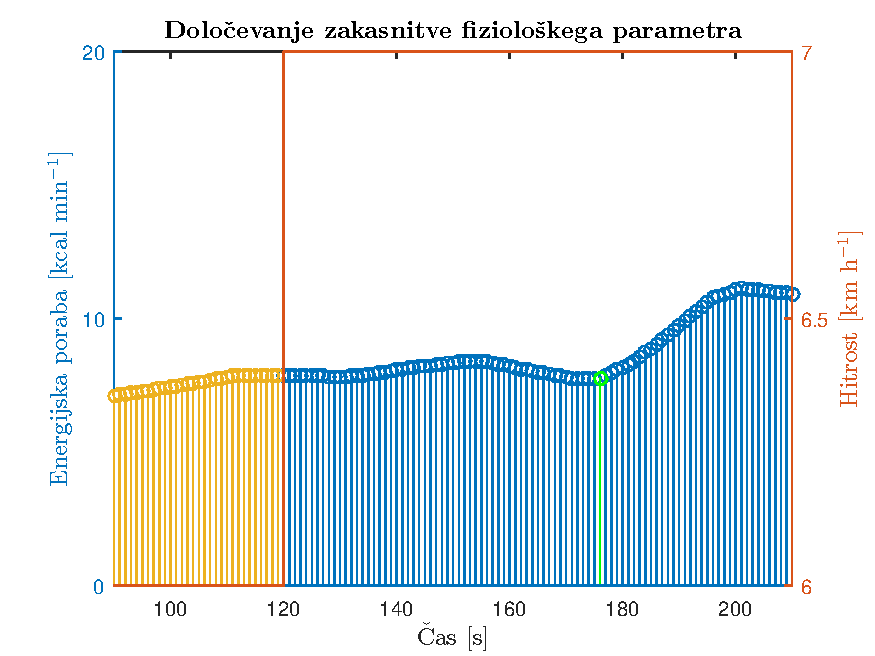
\includegraphics[width=\columnwidth]{stage1-lag-estimation-eem-sl}
		\caption{Zakasnitev za energijsko porabo.}
		\label{fig:lag-estimation-train-eem}
	\end{subfigure}
	~
	\begin{subfigure}[t]{0.45\columnwidth}
		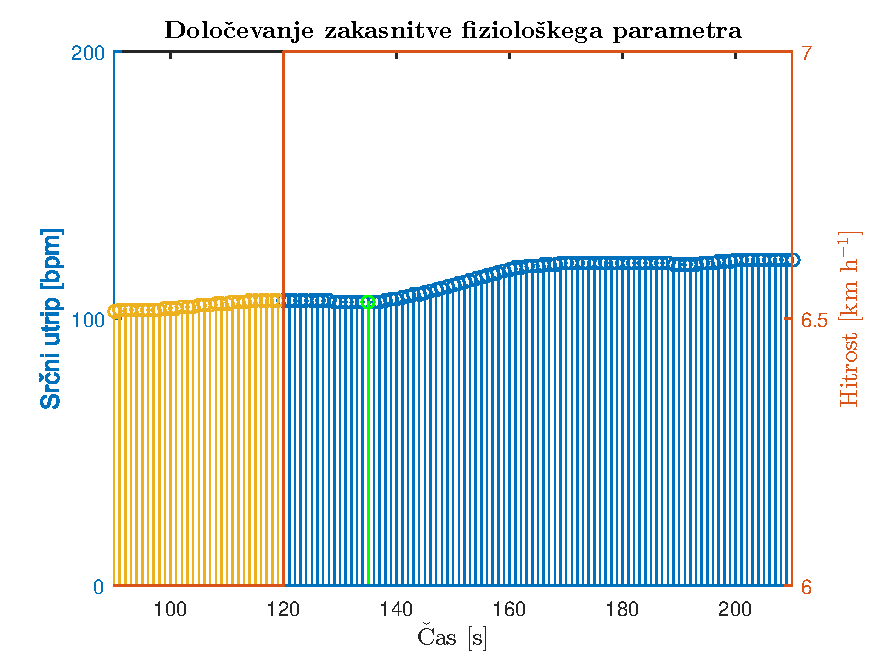
\includegraphics[width=\columnwidth]{stage1-lag-estimation-hr-sl}
		\caption{Zakasnitev za srčni utrip.}
		\label{fig:lag-estimation-train-hr}
	\end{subfigure}
	\caption[Prikaz določevanja dodatne zakasnitve]{Prikaz določevanja dodatne zakasnitve. Na posameznem grafu so prikazani vzorci fiziološkega parametra. Rumena barva označuje vzorce pred spremembo hitrosti tekalne steze, modra pa vzorce po spremembi. Sprememba hitrosti tekalne steze je prikazana z rdečo stopnico. Zeleno obarvani vzorec se nahaja ob trenutku, ko nastane fiziološki odziv.}
	\label{fig:lag-estimation-stage1}
\end{figure}

Zamik za srčni utrip je znašal \SI{15}{\s}. Za energijsko porabo smo izmerili \SI{55}{\s} zamika. Izbrane parametre smo testirali s zakasnitvenimi modeli s kratico \textit{lag}.

Zakasnitev smo določili, kot časovni interval od trenutka spremembe hitrosti tekalne steze do trenutka, ko se je vrednost fiziološkega parametra začela močneje povečevati. Pri tem smo izbrali spremembo hitrosti med prvim in drugim testom, saj je bil signal fiziološkega parametra na tem območju najbolj ustaljen. Kadar je povečevanju dokaj hitro sledil upad, smo smatrali, da do odziva še ni prišlo. Tak primer je prikazan na sliki \ref{fig:lag-estimation-stage1}\subref{fig:lag-estimation-train-eem}), kjer prvemu povečevanju za spremembo hitrosti tekalne steze sledi upad. 


\begin{figure}[!htb]
	\centering
	\begin{subfigure}[t]{0.45\columnwidth}
		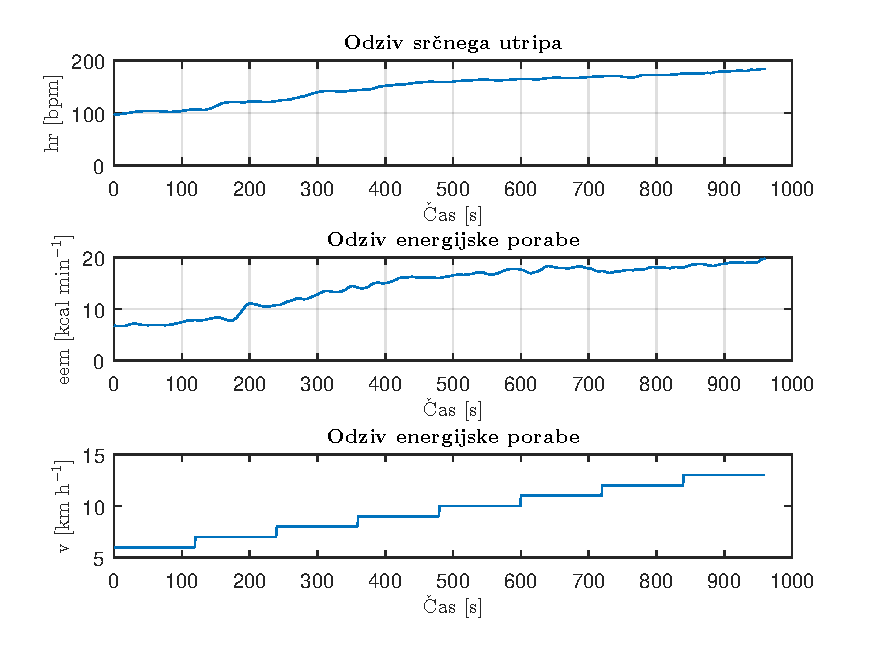
\includegraphics[width=\columnwidth]{odziv1-sl}
		\caption{Odziv učnih vzorcev.}
		\label{fig:odziv-ucnih-stage1}
	\end{subfigure}
	~
	\begin{subfigure}[t]{0.45\columnwidth}
		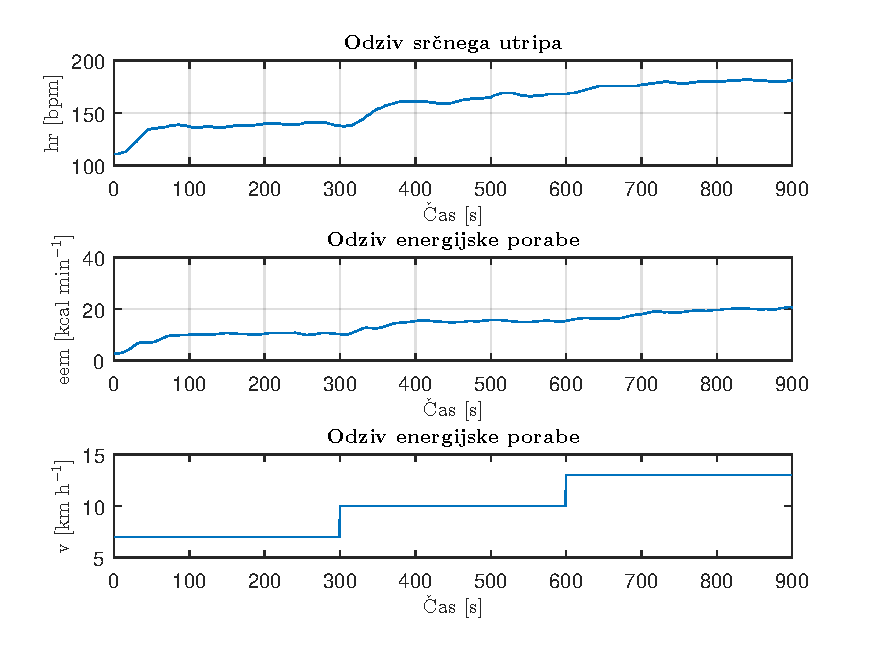
\includegraphics[width=\columnwidth]{odziv2-sl}
		\caption{Odziv testnih vzorcev.}
		\label{fig:odziv-testnih-stage1}
	\end{subfigure}
	\caption[Odziv posameznih fizioloških parametrov za obe seriji testov]{Odziv posameznih fizioloških parametrov za obe seriji testov.}
	\label{fig:odziv-stage1}
\end{figure} 


\subsubsection{Ročna določitev področja tarče}
HOOF deskriptorji so v teoriji robustni na šum, saj ta zaradi majhnih amplitud nima vpliva na obliko histograma. Vseeno pa se lahko pojavijo anomalije, ki povečajo amplitudo šuma na raven vrednosti merjenca. Pri tem mislimo predvsem na objekte in osebe v ozadju, ki se premikajo. Temu se lahko preprosto izognemo z določevanjem področja tarče. Ker je bil prizor na posnetkih razmeroma enostaven in ciklično monoton, smo se za preizkus naše hipoteze odločili, da bomo področja najprej določili ročno. Področja smo izbrali tako, da je bil merjenec ves čas skozi posnetek v izbranem področju. Izbrana področja za posamezne posnetke so predstavljena v tabeli \ref{tab:rocna-podrocja}, pri čemer so $h$ dolžina slike $w$ širina slike ter $x$ in $y$ slikovni koordinati. Vsi nadaljnji testi razen, kjer se uporablja sledilnik, temeljijo na izrezanih posnetkih, glede na ta področja.

\begin{table}[!htb]
	\centering
	\begin{tabular}{l l l S[table-format=3] S[table-format=2] S[table-format=3] S[table-format=3]}
		\toprule
		\multicolumn{3}{c}{}& \multicolumn{4}{c}{\textbf{Področje}} \\
		\cmidrule{4-7}
		\textbf{Serija} & \textbf{Pogled} & \textbf{Vrsta} & \thead{$\mathbf{x}$} & \thead{$\mathbf{y}$} & \thead{$\mathbf{w}$} & \thead{$\mathbf{h}$}  \\
		\midrule
		\multirow{3}{*}{1} & \multirow{2}{*}{hrbtni} & RGB & 228 & 43 & 207 & 437 \\
		&& IR & 32 & 10 & 167 & 329 \\
		& stranski & RGB & 179 & 31 & 346 & 420 \\
		\midrule
		\multirow{3}{*}{2} & \multirow{2}{*}{hrbtni} & RGB & 230 & 51 & 228 & 429 \\
		&& IR & 29 & 11 & 181 & 338 \\
		& stranski & RGB & 182 & 33 & 351 & 423 \\
		\bottomrule
	\end{tabular}
	\caption[Ročno izbrana področja tarče za posamezne posnetke]{Ročno izbrana področja tarče za posamezne posnetke. $x$ in $y$ sta koordinati zgornjega levega kota področja. $w$ in $h$ sta širina in dolžina področja.}
	\label{tab:rocna-podrocja}
\end{table}

\subsubsection{Združevanje posnetkov}
V dodatnih \textit{mixed} modelih, smo združili posnetke kamer z različnim zornim kotom. Združeni posnetek je bil po vrstnem redu sestavljen in posnetka stranske kamere in posnetka hrbtne kamere. Pri tem smo uporabili izrezane posnetke glede na ročno določena področja. Z združenim posnetkom smo želeli preveriti vpliv povečevanja informacije o gibanju merjenca zaradi uporabe različnih zornih kotov. 

\subsubsection{Obremenitveni testi}
Z obremenitvenimi testi smo želeli preizkusiti robustnost našega postopka. Opravili smo dve vrsti testov, in sicer: \textit{scale} teste in \textit{proj} teste. Pri \textit{scale} testih smo posnetke zmanjšali za \SI{50}{\%}. S tem smo simulirali večjo oddaljenost merjenca od kamere in tako preverili teoretično invariantnost HOOF deskriptorjev glede na skalo.

Z vnašanjem projektivne transformacije v posnetke smo s \textit{proj} testi preizkušali robustnost celotnega postopka na deformacije slike, ki jo lahko vnašajo leče kamere. Projektivno transformacijo smo izvedli s pomočjo Matlabovih funkcij \texttt{fitgeotrans} in \texttt{imwarp}. Za vhodne točke smo izbrali robove posamezne slike zaporedja. Za izhodne točke smo izbrali vrednosti v tabeli \ref{tab:projective}, pri čemer so $h$ dolžina slike, $w$ širina slike ter $x$ in $y$ slikovni koordinati.

\begin{table}[!htb]
	\centering
	\begin{tabular}{l S[table-format=1.3] S[table-format=1.3] }
		\toprule
		\thead{Točka} & \thead{$\mathbf{x~[\times w]}$} & \thead{$\mathbf{y~[\times h]}$} \\
		\midrule
		$P_0$ & 0 & 0.25 \\
		$P_1$ & 1 & 0 \\
		$P_2$ & 0.125 & 0.75 \\
		$P_3$ & 0.875 & 0.875 \\
		\bottomrule
	\end{tabular}
	\caption[Tabela pozicij robov transformirane slike]{Tabela pozicij robov transformirane slike. $h$ je dolžina slike, $w$ širina slike ter $x$ in $y$ slikovni koordinati.}
	\label{tab:projective}
\end{table}


\begin{figure}[!htb]
	\centering
	\begin{subfigure}[t]{0.45\columnwidth}
		\centering
		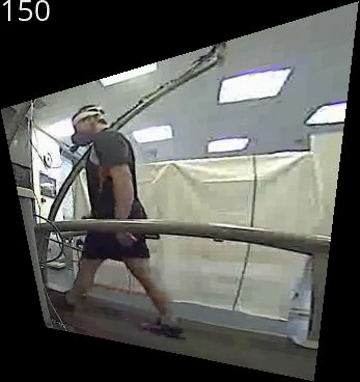
\includegraphics[width=0.6\columnwidth]{projective-sv-150.png}
		\caption{Stranska slika}
	\end{subfigure}
	~
	\begin{subfigure}[t]{0.45\columnwidth}
		\centering
		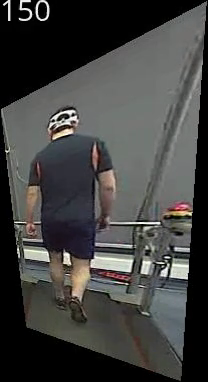
\includegraphics[width=0.4\columnwidth]{projective-bv-150.png}
		\caption{Hrbtna slika}
	\end{subfigure}
	\caption[Primer projektivne transformacije 150. slike posnetka iz prve serije]{Primer projektivne transformacije 150. slike posnetka iz prve serije. Prikazani sta stranska in hrbtna transformirana slika. Transformirali smo slike \ref{fig:primer-posnetka-rgb}.}
	\label{fig:projective}
\end{figure}


\subsubsection{Sledenje merjencem}\label{sec:tracking}
Obstaja veliko ekipnih športov, kjer sodeluje več igralcev. Ker so vsi vidni na vsaki sliki zaporedja posnetka, je nujno, da v naš sistem uvedemo funkcionalnost sledenja. S sledenjem na tekalni stezi smo preverili delovanje te funkcionalnosti. Rezultati, ki vsebujejo korak sledenja imajo kratico \textit{tr}. Primer sledenja je prikazan na sliki \ref{fig:sledenje}.

\begin{figure}[!htb]
	\centering
	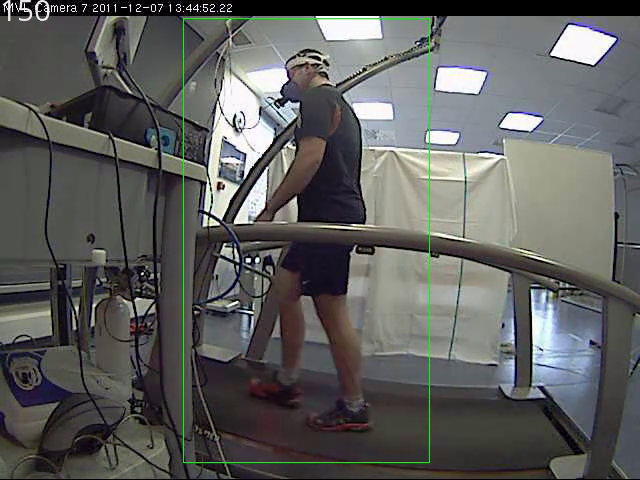
\includegraphics[width=0.6\columnwidth]{normal-sv-test-kcf2.png}
	\caption[Sledenje merjencu s KCF na stranski sliki]{Sledenje merjencu s KCF na stranski sliki. Prikazana je 150. slika RGB posnetka druge serije. Zeleni okvir prikazuje področje, ki ga je detektiral sledilnik.}
	\label{fig:sledenje}
\end{figure} 

Za sledenje smo uporabili KCF sledilnik, ki je implementiran v OpenCV knjižnici. Izbiro sledilnika smo opredelili že v poglavju \ref{sec:testiranje-sledilnikov-za-opticni-tok}. Pri sledenju smo uporabili sledeče parametre: pasovna širina Gaussovega jedra $0.2$, linearni interpolacijski faktor za adaptacijo $0.075$, regularizacijski faktor $0.01$, največja velikost obliža (ang. Patch) $6400$, prostorska pasovna širina $0.0625$, aktivirano skaliranje značilk za izboljšanje hitrosti procesiranja, razcepljeni učni koeficienti na dve matrike, dekativirano zavijanje (ang. wrapping) okoli vrednosti jedra, nekompresirani deskriptorji za sivinske slike in kompresirani za barvne slike, aktivirana PCA metoda za kompresijo značilk, velikost kompresije $2$ in  stopnja učenja kompresije $0.15$.

KCF sledilnik smo inicializirali z ročnim obkroževanjem področja tarče na prvi sliki vsakega posnetka. Področja tarče, ki jih je izbral sledilnik, smo uporabili za izrezovanje področij merjenca iz slik optičnega toka. HOOF deskriptorje smo izračunali le na izbranem področju. 



\subsubsection{Simulacija vibracij kamere}
Kadar uporabljamo ročne kamere, pogosto pride do tresenja. Vibracije smo simulirali z majhnimi naključnimi premiki in rotacijo posameznih slik iz video zaporedja. Vsako sliko smo transformirali z Evklidsko transformacijo. Pri tem smo translacijo omejili na \SI{4}{\%} velikosti slike. Rotacija je bila omejena na \SI{0.13}{rad}. 

Translacijo in rotacijo smo filtrirali še s Kalmanovim filtrom, tako da smo dobili bolj realistično simulacijo. Za Kalmanov filter smo uporabili enak model, kot je predstavljen v poglavju \ref{sec:kalmanov-filter}. Začetne variance filtra smo določili empirično tako, da smo dobili čimbolj realistične rezultate. Varianca šuma merilnega modela je znašala $\sigma_\vec{z}^2=1024$, varianca šuma modela gibanja pa $\sigma_\vec{x}^2=2$. Za kovariančno matriko predikcije smo uporabili varianco $\sigma_\vec{P}^2=2$.

S simulacijo vibracij smo naredili obremenitveni test za modele z vključenim sledilnikom. Rezultati so anotirani s \textit{sh} kratico. Primer delovanja sledilnika je prikazan na sliki \ref{fig:vibracije}.

\begin{figure}[!htb]
	\centering
	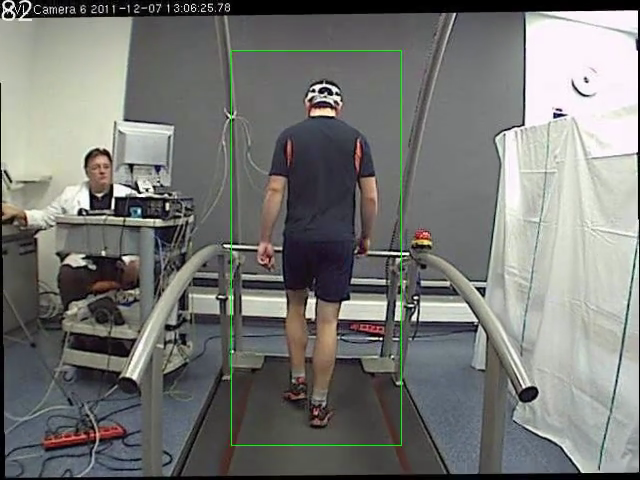
\includegraphics[width=0.6\columnwidth]{shake-bv-train-kcf2.png}
	\caption[Sledenje merjencu na tresočem posnetku]{Sledenje merjencu na tresočem posnetku. Prikazana je 82. slika hrbtnega RGB posnetka prve serije. Zeleni okvir prikazuje področje, ki ga je detektiral KCF sledilnik.}
	\label{fig:vibracije}
\end{figure} 








\subsection{Terenski eksperimenti squash igre}
Pri terenskih eksperimentih smo snemali dve squash igri z enim setom z RaspberryPi in RaspiCam napravo v resoluciji  $1920 \times 1080$. Zaradi nezadovoljivih podatkov druge igre, smo za učenje in testiranje modelov uporabili le prvo igro. Igralcem smo merili srčni utrip s kontaktnimi senzorji. 

Prvega igralca prve igre  (starost: 45 let, velikost: \SI{176}{\cm}, teža: \SI{68}{\kg}, spol: male, $hr_{tmax}$: \SI{179}{bpm}, $hr_{r}$: \SI{45}{bpm}) smo uporabili za učne vzorce. Drugega igralca (starost: 17 let, višina: \SI{178}{\cm}, teža: \SI{66}{\kg}, spol: male, $hr_{tmax}$: \SI{203}{bpm}, $hr_{r}$: \SI{50}{bpm}) smo uporabili za testne vzorce. 

\subsubsection{Razširitev HOOF deskriptorja}
Chaudhry et al. \cite{chaudhry2009histograms} predlaga uporabo histogramov orientiranega optičnega toka (HOOF) za estimacijo gibanja. Vendar pa smo v terenskih testiranjih ugotovili, da njihova uporaba v realnih okoliščinah ni zadovoljiva. HOOF deskriptorju smo pripeli HAFA deskriptor in tako dobili razširjeni deskriptor HOOF-HAFA, ki v splošnem daje boljše rezultate, kot je bilo prikazano v poglavju \ref{sec:razsiritev-hoof-rezultati}. Primer deskriptorja je viden na sliki \ref{fig:hoof-hafa}.

\begin{figure}[!htb]
	\centering
	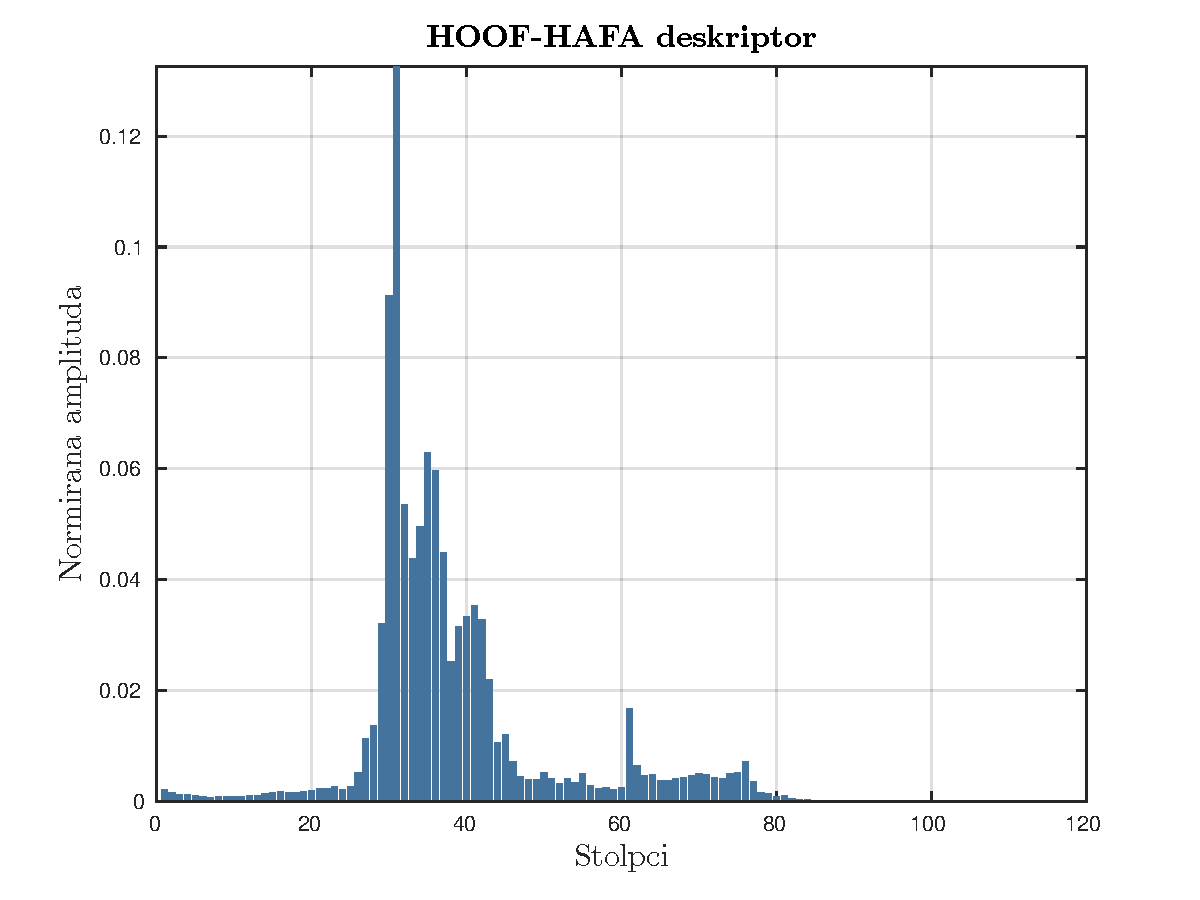
\includegraphics[width=0.6\columnwidth]{stage1-field-bv-of-hist-sl}
	\caption[HOOF-HAFA deskriptor za 276. sliko učnih vzorcev]{HOOF-HAFA deskriptor za 276. sliko učnih vzorcev. Deskriptor se ujema s sliko \ref{fig:sledenje-squash}.}
	\label{fig:hoof-hafa}
\end{figure}

\subsubsection{Postopek procesiranja}
Za določitev področja posameznega igralca smo uporabili KCF sledilnik. Kadar sledilnik ni uspel najti objekta zanimanja, je bilo področje prazno, zato so bile vse vrednosti HOOF-HAFA deskriptorjev $0$. To se je zgodilo v primerih, ko je tarča izginila iz vidnega polja kamere ali pa ko sledilnik ni več deloval. Zaradi teh težav smo sledenje nadzorovano reinicializirali vsake \SI{3}{\s}. S tem smo zagotovili razumne sledilne rezultate. Zaradi prevelike resolucije posnetkov, smo morali za pravilno delovanje sledilnika posnetke skalirati na \SI{25}{\%} prvotne velikosti. Rezultate sledenja smo nato morali transformirati nazaj na originalno resolucijo. Primer sledenja je prikazan na sliki \ref{fig:squash}\subref{fig:sledenje-squash})

\begin{figure}[!htb]
	\centering
	\begin{subfigure}[t]{0.45\columnwidth}
		\centering
		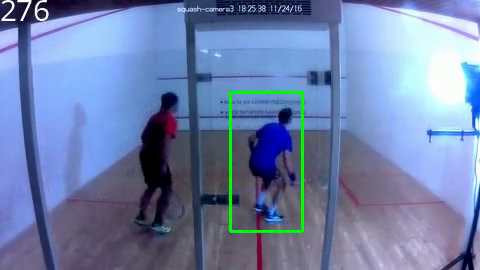
\includegraphics[width=\columnwidth]{squash-tracked.png}
		\caption{Slika sledenja.}
	    \label{fig:sledenje-squash}
	\end{subfigure}
	~
	\begin{subfigure}[t]{0.45\columnwidth}
		\centering
		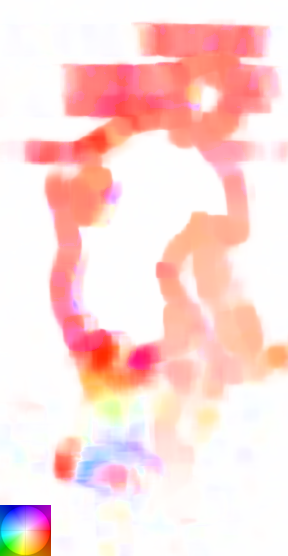
\includegraphics[width=0.4\columnwidth, frame]{stage1-squash-flo-corrected.png}
		\caption{Slika optičnega toka.}
		\label{fig:of-squash}
	\end{subfigure}
	\caption[Slika sledenja in optičnega toka za igralca terenskih eksperimentov]{Slika sledenja in optičnega toka za igralca prve igre terenskih eksperimentov. Sledili smo modremu igralcu, ki smo ga uporabili za učne vzorce. Zeleni okvir na sliki \subref{fig:sledenje-squash}) prikazuje področje detekcije 276. slike posnetka. Korespondečni optični tok področja je prikazan na sliki \subref{fig:of-squash} z legendo barvnega kodiranja v spodnjem levem kotu. Na sliki uporabljamo standardno barvno kodiranje, povzeto po \cite{baker2011database}. Maksimalna amplituda optičnega toka je na tej sliki znašala \SI{31}{ppf}. }
	\label{fig:squash}
\end{figure}

Izmerjeni srčni utrip smo filtrirali z Gaussovim filtrom s standardnim odklonom \num{16}. S tem smo preprečili učenje na šumnih podatkih. Srčni utrip je bil individualiziran na parametre učnega igralca s pretvorbo v energijsko porabo po enačbi \eqref{eq:charlot}. Rezultate smo nato z isto enačbo pretvorili nazaj v srčni utrip s parametri testnega igralca. S tem smo omogočili učenje na enem in testiranje na drugem igralcu. 

Po določevanju optičnega toka (slika \ref{fig:squash}), smo uporabili HOOF-HAFA deskriptorje, katerih značilke smo skalirali na intervalu $[-1,1]$. Učili smo s postopkom \esvr in jedrom RBF. Za terenske eksperimente Kalmanovega filtra nismo uporabili. Ker je bil Gaussov filter uporabljen pri predprocesiranju podatkov, smo enak filter uporabili tudi za filtriranje izhodov modela.

\begin{figure}[!htb]
	\centering
	\resizebox{\columnwidth}{!}{\begin{tikzpicture}
% LAYERS
\pgfdeclarelayer{bg}
\pgfsetlayers{bg,main}
\tikzset{
    between/.style args={#1 and #2}{
         at = ($(#1)!0.5!(#2)$)
    }
}

% NODES
\node (slika) [input] at (0,0) {Slika\\$I(x,y)$};
\node (tracker) [block, right= of slika] {KCF\\sledilnik};
%\node (tarca) [block, right= of tracker] {Področje\\tarče};

\node (of) [block, right= of tracker] {Optični\\tok $\vec{w}$};
\node (hoof) [block, right= of of] {HOOF-HAFA\\deskriptorji\\$\vec{x}(t)$};


\node (ucenje) [block, right=of hoof] {\esvr\\RBF};
\node (kalman) [block, right= of ucenje] {Gaussov\\filter};


\node (rezultat) [output, right= of kalman] {Rezultat};

% arrows
\draw [arrow] (slika) -- (tracker);
\draw [arrow] (tracker) -- (of);
%\draw [arrow] (tarca) -- (of);
\draw [arrow] (of) -- (hoof);
\draw [arrow] (hoof) -- (ucenje);
\draw [arrow] (ucenje) -- (kalman);
\draw [arrow] (kalman) -- (rezultat);
\end{tikzpicture}}
	\caption[Diagram procesiranja terenskih eksperimentov 1. faze]{Diagram procesiranja terenskih eksperimentov 1. faze. Področju, ki smo ga dobili s KCF sledinikom, smo določili optični tok. Sledilo je učenje na HOOF-HAFA deskriptorjih, Rezultate smo filtrirali s Gaussovim filtrom.}
	\label{fig:diagram-procesiranja-field-stag1}
\end{figure}

















\subsection{Detekcija dihanja}
Za prikaz splošne uporabnosti elementarnega postopka iz poglavja \ref{sec:elementarni-postopek}, smo ga uporabili za detekcijo dihanja. Za razliko od uporabe postopka v športu, lahko detekcijo dihanja uporabljamo za medicinske namene, v skrbi za starejše ali pri nadzornih kamerah. Koncept optičnega merjenja nam omogoča, da aplikacijo uporabimo z daljših razdalj, dokler nam optični sistem to omogoča. 

Seveda obstaja že kar nekaj aplikacij monitoringa pacientov s pomočjo računalniškega vida. Naša glavna motivacija je bilo testiranje predlagane metode na drugačnem problemu.

\subsubsection{Pridobivanje podatkov}
Za testiranje detekcije dihanja smo posneli video moškega merjenca, starosti 42 let z diagnozo spalne apneje. Snemanje se je začelo ob 4:45 zjutraj med spanjem merjenca in je trajalo 30 min. Prostor smo osvetlili z \SI{60}{w} bližnje-infrardečim (NIR) osvetljevalnikom. Snemali smo z RaspberryPi RaspiCam  napravo (NIR verzija, brez filtra za blokiranje NIR). Hitrost snemanja je bila \SI{25}{fps}, ki smo jo zmanjšali na \SI{10}{fps} v predprocesiranju videa. Ker je dihanje počasen proces, smo z zmanjševanjem hitrosti izboljšali SNR v pridobljenem optičnem toku. Pri snemanju smo uporabili širokokotno M12 lečo z goriščno razdaljo \SI{1.8}{mm}. Snemalna aparatura je bila oddaljena približno \SI{2}{m} od opazovanega subjekta. Primer slike posnetka je prikazan na sliki \ref{fig:dihanje-orig}.

\begin{figure}[htb]
	\centering
	\begin{subfigure}[t]{0.3\columnwidth}
		\centering
		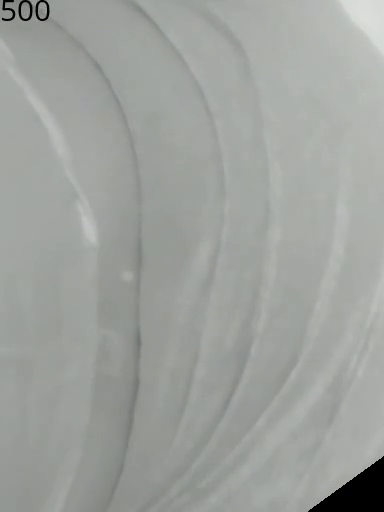
\includegraphics[width=\columnwidth]{breathtest-500.png}
		\caption{IR slika dihanja.}
		\label{fig:dihanje-orig}
	\end{subfigure}
	~
	\begin{subfigure}[t]{0.3\columnwidth}
		\centering
		
\includegraphics[width=\columnwidth, frame]{breathtest-flow-coding.png}
		\caption{Optični tok dihanja.}
		\label{fig:dihanje-of}
	\end{subfigure}
	~
	\begin{subfigure}[t]{0.3\columnwidth}
		\centering
		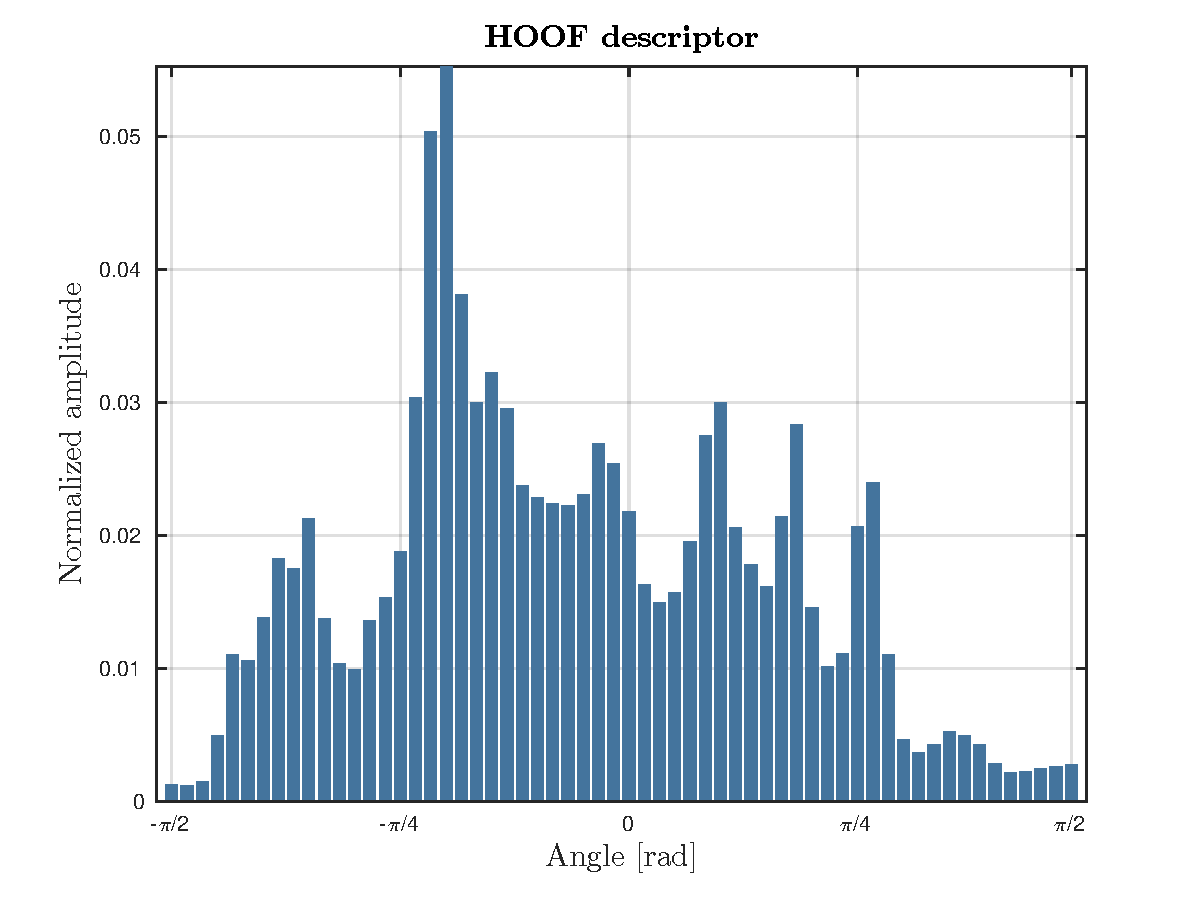
\includegraphics[width=\columnwidth]{stage1-breathtest-hist-en}
		\caption{HOOF histogram.}
		\label{fig:dihanje-hist}
	\end{subfigure}
	\caption[Originalna IR slika dihanja, njen optični tok in HOOF histogram]{Originalna IR slika dihanja, njen optični tok in HOOF histogram Prikazana je 500. slika učnih vzorcev. Optični tok ima z legendo barvnega kodiranja v spodnjem levem kotu. Na sliki uporabljamo standardno barvno kodiranje, povzeto po \cite{baker2011database}. Maksimalna amplituda optičnega toka je na tej sliki znašala \SI{1}{ppf}.}
	\label{fig:dihanje}
\end{figure} 

\subsubsection{Referenčni podatki}
Za pridobitev referenčnih podatkov smo snemali tudi zvok z avdio modulom za RaspberryPi. Mikrofon smo postavili v neposredno bližino merjenca. Zvok smo sinhronizirali z video posnetkom. Detekcije dihanja so predstavljale visoko amplitudo zvoka. Dobljene detekcije smo pregledali z operaterjem in potrdili, da korespondirajo z dejanskim dihanjem na avdio posnetku. Detekcije dihanja smo prevzorčili na \SI{10}{Hz}, da so se skladale s frekvenco vzorčenja video posnetka.

\subsubsection{Procesiranje}\label{sec:data-preprocessing}
Opazovali smo področje subjektovega hrbta. Subjekt je ležal obrnjen navzdol. Področje je bilo veliko $384 \times 512$ slikovnih elementov in je pokrivalo približno $2/3$ hrbta. To je bil edini del slike, ki smo ga uporabili.

Iz posnetka smo izbrali dva zaporedja slik s trajanjem \SI{5}{min}. Prvo zaporedje smo uporabili za učenje, drugo pa za testiranje. Pri uporabi optičnega toka smo spremenili parameter velikost okna na $64$. Iz optičnega toka smo izračunali HOOF histograme. Njihove značilke smo normirali na intervalu $[-1,1]$. Učili smo z C-SVC razvrščevalnikom in RBF jedrom, pri tem pa uporabili optimizacijo parametrov. Za določitev uspešnosti delovanja smo problem formulirali kot problem binarnega razvrščanja z razredoma ``diha'' in ``ne diha''. Rezultatov nismo filtrirali.

\begin{figure}[htb]
	\centering
	\resizebox{\columnwidth}{!}{\begin{tikzpicture}
% LAYERS
\pgfdeclarelayer{bg}
\pgfsetlayers{bg,main}
\tikzset{
	between/.style args={#1 and #2}{
		at = ($(#1)!0.5!(#2)$)
	}
}

% NODES
\node (slika) [input] at (0,0) {Področje\\na sliki $I(x,y)$};

\node (of) [block, right= of slika] {Optični\\tok $\vec{w}$};
\node (hoof) [block, right= of of] {HOOF\\deskriptorji $\vec{x}(t)$};


\node (ucenje) [block, right= of hoof] {C-SVC\\RBF};

\node (rezultat) [output, right= of ucenje] {Rezultat};

% arrows
\draw [arrow] (slika) -- (of);


\draw [arrow] (of) -- (hoof);
\draw [arrow] (hoof) -- (ucenje);

\draw [arrow] (ucenje) -- (rezultat);
\end{tikzpicture}}
	\caption[Diagram procesiranja pri uporabi metode za detekcijo dihanja]{Diagram procesiranja pri uporabi metode za detekcijo dihanja.}
	\label{fig:dihanje-postopek}
\end{figure}

% \begin{table}[h]
%     \centering
%     \begin{tabular}{l r D{.}{.}{-1} D{.}{.}{-1}}
% 		\toprule
%         \textbf{Model name} & \multicolumn{3}{c}{\textbf{Parameters}} \\
%         & \multicolumn{1}{c}{$C$} & \multicolumn{1}{c}{$\gamma$} & \multicolumn{1}{c}{$\epsilon$} \\
%         \midrule
%         hr-sv		&	1024	&	16	&	3.48	\\
%         hr-sv-lag 	&	4096	&	11.31
%         &	2.14	\\
%         hr-bv		&	4096	&	16	&	4.59	\\      
%         hr-bv-lag 	&	1024	&	16	&	2.46	\\
%         eem-sv		&	256	&	16	&	0.81	\\
%         eem-sv-lag	&	256	&	16	&	0.54	\\
%         eem-bv		&	256	&	16	&	1.62	\\   
%         eem-bv-lag	&	256	&	16	&	1.74	\\
%         hr-mixed	&	1024	&	16	&	4.59	\\
%         hr-mixed-lag &	1024	&	16	&	4.59	\\
%         eem-mixed	&	90.51	&	16	&	1.15	\\
%         eem-mixed-lag	&	64	&	16	&	0.93	\\
%         hr-sv-tr	&	1024	&	11.31	&	3.73	\\
%         hr-sv-lag-tr	&	1024	&	16	&	3.03	\\
%         hr-bv-tr	&	256	&	16	&	2.64	\\
%         hr-bv-lag-tr	&	256	&	16	&	3.48	\\
%         eem-sv-tr	&	256	&	11.31	&	0.50	\\
%         eem-sv-lag-tr	&	256	&	16	&	0.31	\\
%         eem-bv-tr	&	64	&	16	&	1.87	\\
%         eem-bv-lag-tr	&	64	&	16	&	1.87	\\
%         hr-sv-tr-sh	&	64	&	16	&	4.59	\\
%         hr-sv-lag-tr-sh	&	64	&	16	&	4.59	\\
%         hr-bv-tr-sh	&	16	&	16	&	1.23	\\
%         hr-bv-lag-tr-sh	&	16	&	11.31	&	2.14	\\
%         eem-sv-tr-sh	&	16	&	16	&	0.62	\\
%         eem-sv-lag-tr-sh	&	16	&	16	&	0.87	\\
%         eem-bv-tr-sh	&	1.41	&	16	&	0.09	\\
%         eem-bv-lag-tr-sh	&	4	&	16	&	1.23	\\
%         hr-bv-lag-tr-sq	&	1024	&	0.25	&	4.59	\\
%         \bottomrule
% 	\end{tabular}
%      \caption{The optimal parameters for individual models, which were obtained by grid search with five-fold cross-correlation, as indicated in \cite{hsu2003practical}. Parameters were used for learning models with the LIBSVM library.}
%     %\caption{Optimalni parametri za posamezne modele, ki smo jih dobili z mrežnim iskanjem s petkratno križno korelacijo, kot je navedeno v \cite{hsu2003practical}. Parametre smo uporabili za učenje modelov v knjižnici LIBSVM.}
%     \label{tab:optimalni-parametri}
% \end{table}

% As said in \ref{sec:data-preprocessing}, predicted results for squash experiment were converted with basic equation from \cite{charlot2014improvement}, because energy expenditure models were used.


\section{Eksperimenti 2. faze}
Z laboratorijskimi eksperimenti v 1. fazi smo dobili zadovoljive rezultate, težave pa so nastale pri uporabi postopka na terenu. Zato smo v 2. fazi optimizirali posamezne segmente elementarnega postopka estimacije fizioloških parametrov. Te smo tudi uporabili v končni preiskavi. V preliminarnih testih so opisani tudi drugi postopki, ki smo jih potrebovali zaradi uporabe Kinect kamer.

Za statistično bolj oprijemljive rezultate smo v laboratorijskih in terenskih eksperimentih 2. faze uporabili 7 različnih merjencev z oznakami: SUBJ1, SUBJ2, SUBJ4, SUBJ7, SUBJ8, SUBJ9, SUBJ10. 

Merjenca SUBJ4 smo uporabili samo v laboratorijskih eksperimentih, ker pri terenskih eksperimentih ni bil prisoten. Namesto njega smo v terenskih eksperimentih uporabili merjenca SUBJ10. V laboratorijskih eksperimentih merjenca SUBJ10 nismo upoštevali zaradi napak pri zajemu meritev.

Med laboratorijskimi in terenskimi eksperimenti je za merjenca SUBJ1 in SUBJ2 preteklo 43 dni, za merjenca SUBJ4 42 dni in za ostale 1 dan.  

\subsection{Preliminarni testi}
\subsubsection{Združevanje slik iz dveh Kinect kamer}\label{sec:zdruzevanje}

\paragraph{Združevanje z značilkami}
Časovno sinhornizirana zaporedja slik smo poskušali združiti z metodo panoramskega šivanja slik z uporabo značilk, kot je opisano v delu \cite{brown2007automatic}. Tu smo namesto SIFT značilk uporabili SURF značilke.


\paragraph{Združevanje s kontrolnimi točkami}
Zaporedja slik smo poskušali združiti z ročnim določevanjem kontrolnih točk.


\paragraph{Prilagojeno združevanje}
Zaradi nezadovoljivih rezultatov klasičnih metod združevanja stereo slik, smo razvili metodo, ki je prilagojena za Kinect kamere. Iz kamer smo pridobili intrinzične parametre infra-redečega (IR) senzora, in sicer: slikovni koordinati goriščne razdalje $f_u$ in $f_v$ ter slikovni koordinati optičnega središča slike (ang. principal point) $c_u$ in $c_v$. Intrinsične parametre smo uporabili za določitev intrizične matrike $\vec{M}_{int}$ po enačbi \eqref{eq:intrinsic}.


Ker pravih ekstrinsičnih parametrov kamer nismo poznali, smo jih le ocenili z metodo določevanja sečišča vidnih polj obeh kamer. Sečišče je prikazano kot rdeča linija na sliki \ref{fig:zdruzevanje}. S to metodo smo določili translacijski vektor $\vec{t} = \left [ t_x~ t_y~ t_z \right]^\top$ in rotacijsko matriko $\vec{R}$ iz Eulerjevih kotov.

S sledenjem igralca z DS-KCF algoritmom, smo s pomočjo projekcijske matrike \eqref{eq:projection-matrix} določili center tarče v metričnih enotah za vsako sliko zaporedja leve in desne kamere. Kadar slikovni element ni vseboval podatkov globine, smo za center tarče izbrali najbližji slikovni element z veljavno globino.

Prva slika združenega zaporedja je bila slika kamere, kjer se igralec prvič pojavi. Nadaljne slike smo izbirali med zaporedjema kamer glede na pozicijo centra tarče. Ko je šel center tarče skozi upragovljeno mejo, ki je na sliki \ref{fig:zdruzevanje} prikazana z modro linijo smo preklopili na drugo kamero. Razdalja med pragom in sečiščem je znašala \SI{200}{mm}.


\begin{figure}[htb]
	\centering
	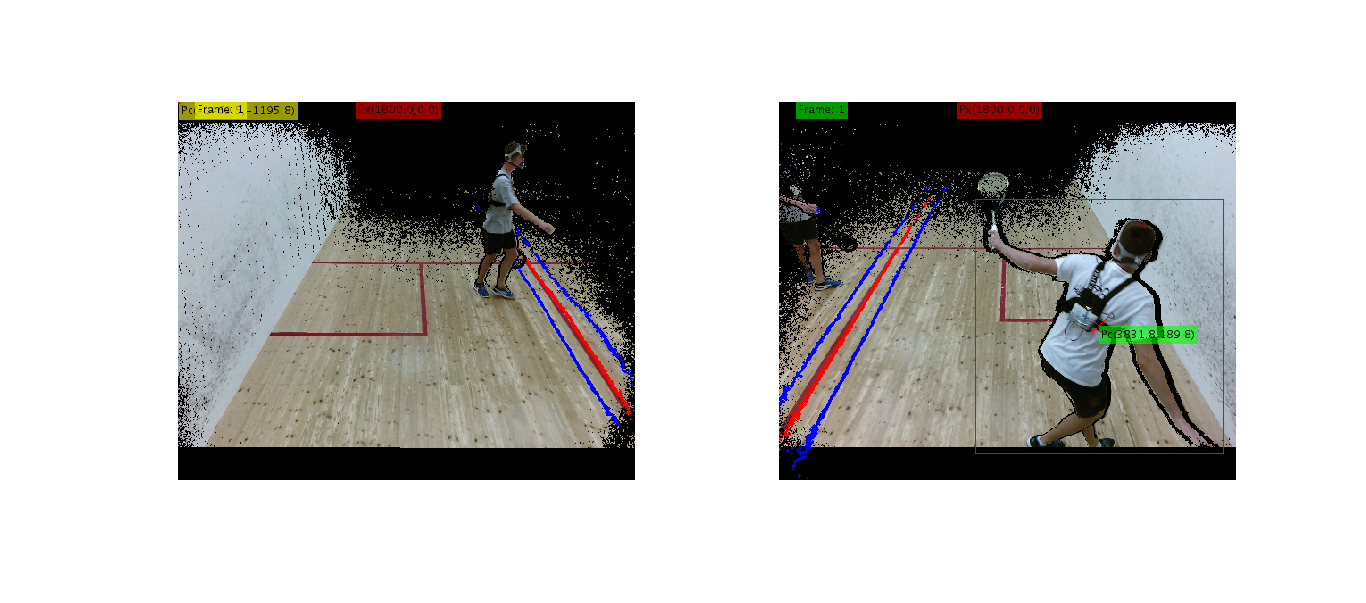
\includegraphics[width=\columnwidth]{./Slike/zdruzevanje-example.png}
	\caption[Določevanje sečišča vidnih polj leve in desne Kinect kamere]{Določevanje sečišča vidnih polj leve in desne Kinect kamere. Na sliki sta prikazani prvi sliki zaporedja leve in desne Kinect kamere 1. seta 2. igre terenskega eksperimenta iz 2. faze. Označen je 4. igralec. Zelena barva koordiat središča tarče predstavlja izbrano kamero. Kamera z rumeno barvo ni izbrana. Sečišče je rdeča linija. Modri liniji sta pragova za preklop med kamerama. Ležita \SI{200}{mm} levo in desno od sečišča.}
	\label{fig:zdruzevanje}
\end{figure}



\subsubsection{Mrežno iskanje \texorpdfstring{$\nu$}{nu}-RBF}
Med evaluacijo eksperimentov 1. faze smo ugotovili, da z regresijo \esvr pogosto dobimo preobremenjene (ang. Overfitted) modele. Pri takih modeli je število podpornih vektorjev zelo visoko. Lahko se zgodi, da postanejo vsi vektorji značilk podporni vektorji. Preobremenjeni modeli lahko dajejo solidne rezultate, vendar pa so ti nerealistični. Takoj, ko bi v tak model vnesli rahlo spremenjene podatke, ne bi več delovali.

Zaradi tovrstnih problemov smo v našem postopku regresijo \esvr zamenjali z \nusvr. Izkazalo se je, da tudi ta ne deluje, čeprav pri njej uporabljamo dodatni parameter $\nu$, s katerim v teoriji kontroliramo razmerje števila podpornih vektorjev, kot je opisano v poglavju \ref{sec:regresija-nusvr}. Chang et. al nam v delu \cite{chang2002training} parameter $\nu$ bolj natačno opiše kot spodnjo mejo razmerja števila podpornih vektorjev. Parameter $\nu$ tako v resnici ne predstavlja omejitve, s katero bi kaznovali prekomerno učneje modela. V ta namen smo razvili mrežno iskanje \nurbf, ki je predstavljeno v poglavju \ref{sec:nurbf}. 

Razvito mrežno iskanje \nurbf uporablja regresijo \nusvr in jedro RBF, zato smo ju uporabljali tudi za učenje modelov. Celoten postopek krajše imenujemo kar \nurbf.

\paragraph{Optimizacija parametrov}
Najprej smo optimizirali parameter $\numax$ oziroma $\numax'$. Slednji predstavlja različico parametra $\numax$, s katerim določimo dejansko število podpornih vektorjev. Za tovrstno optimizacijo smo ponovno naučili \textit{mixed} modele iz 1. faze, pri čemer smo za mrežno iskanje uporabili nov postopek. Modele smo nato uporabili za testiranje na učnih podatkih terenskih eksperimentov 1. faze. S takim postopkom smo izluščili slabe \textit{squash} modele, ki bi oteževali pravilno evaluacijo rezultatov pri optimizaciji.

Za optimizacijo smo uporabili HOOF-HAFA deskriptor in naslednje vrednosti parametrov: začetna vrednost $\nu$ $0.1$ in standardni odklon za Gaussov filter $\sigma=5$. Za $\numax'$ smo uporabili 400, 800 in 1200 podpornih vektorjev. 

Z optimiziranim parametrom $\numax'=400$ smo \nurbf preizkusili še na elementarnih modelih. Tu smo za razliko od eksperimentov iz 1. faze poleg \nurbf uporabili razširjeni HOOF-HAFA deskriptor.







\subsubsection{Jedro GHI}
V poglavju \ref{sec:ghi} smo opisali, da je jedro GHI primerno za histogramske deskriptorje, zato smo ga tudi preizkusili na elementarnih modelih. Tu smo namesto prvotnega HOOF deskriptorja uporabili HOOF-HAFA deskriptor, ki daje boljše rezultate. Pri uporabi GHI jedra smo značilke skalirali na intervalu $[-1,~1]$ zaradi hitrejšega učenja. Učili smo z \esvr metodo. Rezultate smo filtrirali s prvotnim Kalmanovim filtrom.

Zaradi že prej omenjenih težav s prevelikim številom podpornih vektorjev v modelih, smo pri klasičnem mrežnem iskanju sprva uporabili enostavno mero: faktor števila podpornih vektorjev $f_{nSV}$, ki je opisan z enačbo \eqref{eq:fnsv}. $n_v$ je število vzorcev in $n_{SV}$ je število podpornih vektorjev. S to mero določimo procentualno vrednost vektorjev, ki lahko postanejo podporni. Zaradi tega faktorja optimizacija parametra regresije ni bila potrebna. Pri testiranju smo uporabili vrednost $f_{nSV} = 0.01$.


\begin{equation}
f_{nSV} = \frac{n_v - n_{SV}}{n_v}
\label{eq:fnsv}
\end{equation} 

Zgoraj opisana metoda ni delovala zato smo namesto faktorja $f_{nSV}$ uporabili postopek \nughi. Gre za prilagojeno različico postopka \nurbf, kjer smo uporabili GHI jedro. Dodatna razlika je še v tem, da predikcij pri križni validaciji nismo filtrirali, ker smo pri rezultatih uporabili Kalmanov filter. Prav tako smo s tem zagotovili zadovoljiv čas reševanja problema.






\subsubsection{Optimizacija Gaussovega filtra}
Pri optimizaciji Gaussovega filtra smo določili optimalni standardni odklon $\sigma$ z uporabo dveh metrik, in sicer: koren srednje kvadratične napake (RMSE) in razmerje med signalom in šumom (SNR). Pri RMSE metriki smo določili napako med učnimi vzorci in njihovo predikcijo. Pri SNR metriki smo za signal uporabili referenčne učne vzorce. Za šum smo uporabili rezidualni ali preostali šum. Tega smo dobili z odštevanjem filtriranih vzorcev od referenčnih. SNR metrika tako določa uspešnost izločevanja šuma, RMSE metrika pa pravilnost določevanja kateri podatki spadajo v signal in kateri v šum.


Teste smo izvajali na vseh eksperimentih 1. sklopa, pri čemer smo uporabili \nurbf mrežno iskanje s \SI{50}{\%} podpornih vektorjev. Za filtriranje pri mrežnem iskanju smo izbrali najmanjši filter s $\sigma = 1$. Testirali smo naslednje standardne odklone Gaussovega filtra: $1, 3, 5, 11, 21, 31$ in $51$. 




\subsubsection{Normalizacija HAFA deskriptorjev}
V praksi se pokaže, da prvotni HAFA histogram ne deluje zadovoljivo, saj se histogram lahko močno spreminja pri uporabi sledilnika. Zaradi neidelanega delovanja sledilnika področje tarče skozi čas spreminja svojo velikost, to pa vpliva na vrednosti stolpcev HAFA histograma. Ker te dobimo s preštevanjem slikovnih elementov z enako amplitudo hitrosti bo manjše področje posledično zmanjšalo celoten histogram. Pri HOOF histogramih tega problema praktično nimamo, saj ima majhen vpliv. Razlog tiči v računanju vrednosti stolpcev HOOF histograma. Njihove vrednosti dobimo s seštevanjem amplitud in ne njihovim preštevanjem. Te so zato pred normiranjem praviloma večje.

Probleme sledilnika smo poskušali kompenzirati z uvedbo amplitudnega faktorja $f_A$. Amplitudni faktor je pravzaprav razmerje med velikostjo področja igralca na terenskih testih in velikostjo merjenca na tekalni stezi. Razmerje lahko preprosto dobimo z razmerjem diagonal področij po enačbi \eqref{eq:diag}, kjer so $w_l$ in $h_l$ širina in dolžina področja na tekalni stezi ter $w_s$ in $h_s$ širina in dolžina področja na terenskih testih.

\begin{equation}
f_A = \frac{\sqrt{w_l^2 + h_l^2}}{\sqrt{w_s^2 + h_s^2}}
\label{eq:diag}
\end{equation}

Velikost diagonale na laboratorijskih testih uporabljamo kot referenco. To pa zato, ker je na teh posnetkih stabilna, saj se le malo spreminja. Koncept amplitudnega faktorja smo preizkusili na enakem postopku, kot pri optimizaciji parametra mrežnega iskanja \nurbf. S takim postopkom smo izluščili slabe \textit{squash} modele, ki bi oteževali pravilno evaluacijo rezultatov pri optimizaciji. Naučili smo modele \textit{diag}, kjer smo uporabili amplitudni faktor in referenčne modele \textit{normal} brez uporabe faktorja za primerjavo. Diagonalo na tekalni stezi smo določili po sliki \ref{fig:diag-bbox}, kjer smo za zgornji levi kot $P_0$ in spodnji desni kot $P_1$ izbrali vrednosti v tabeli \ref{tab:diag}. 


\begin{figure}[htb]
	\centering
	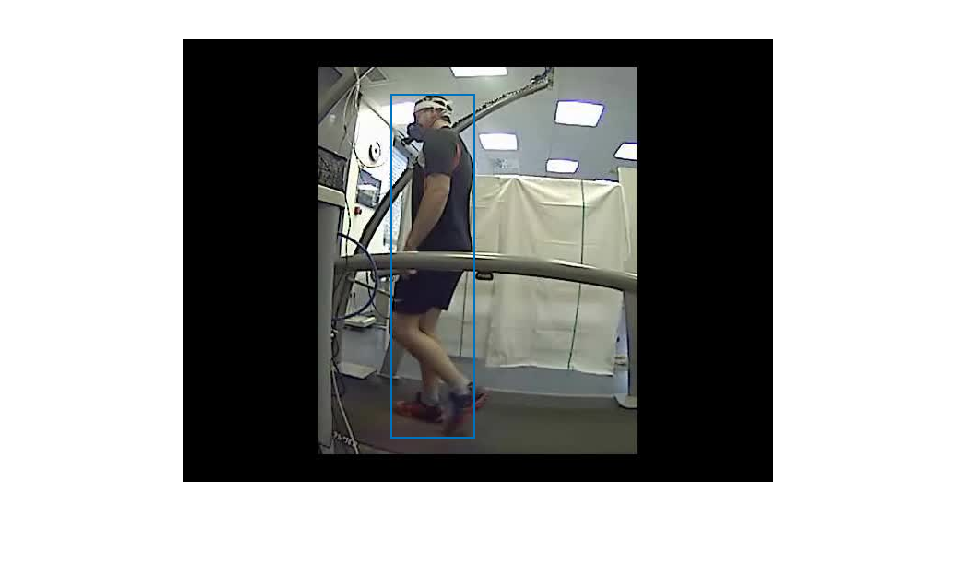
\includegraphics[width=0.75\columnwidth]{./Slike/diag-bbox.png}
	\caption{}
	\label{fig:diag-bbox}
\end{figure}

\begin{table}[htb]
	\centering
	\begin{tabular}{l S[table-format=3] S[table-format=3]}
		\toprule
		\textbf{Točka} & \thead{$\mathbf{x}$} & \thead{$\mathbf{y}$} \\ 
		\midrule
		$P_0$ & 297 & 82 \\
		$P_1$ & 389 & 452 \\
		\bottomrule
	\end{tabular}
	\caption[Optimalni parameteri RBF jedra modelov za izbiro deskriptorjev]{Optimalni parametri RBF jedra za modele z različnim deskriptorjem.}
	\label{tab:diag}
\end{table}

Pri testiranju smo uporabili parameter $\numax$ \SI{50}{\%} podpornih vektorjev. Za Gaussov filter smo uporabili $\sigma=5$. Značilke smo skalirani na intervalu $[0,~1]$. Za modele z diagonalo smo uporabili parameter $f_{A}=381.266$. Pri učenju smo uporabili optimalne vrednosti parametrov, ki so prikazane v tabeli \ref{tab:diag}. Za evaluacijo rezultatov smo uporabili predikcije testnih vzorcev z modeli s zakasnitvijo.



\begin{table}[htb]
	\centering
	\begin{tabular}{l S[table-format=3] S[table-format=1.3] S[table-format=1.1] S[table-format=1.3]}
		\toprule
		\textbf{Model} & \thead{$\mathbf{C}$} & \thead{$\mathbf{\gamma}$} & \thead{$\mathbf{\nu}$} & \thead{MSE} \\ 
		\midrule
		NORMAL & 256 & 0.354 & 0.1 & 5.297 \\
		DIAG & 256 & 0.354 & 0.1 & 5.297 \\
		\bottomrule
	\end{tabular}
	\caption[Optimalni parameteri RBF jedra modelov za izbiro deskriptorjev]{Optimalni parametri RBF jedra za modele z različnim deskriptorjem.}
	\label{tab:izbira-param-diag}
\end{table}


\subsection{Laboratorijski eksperimenti}
Merjenci so opravili obremenilni test po protokolu Nowatzky. To je stopnjevani test na tekoči preprogi za merjenje maksimalne porabe kisika in oceno aerobne kapacitete posameznika. Test smo izvajali s pomočjo sistema za direktno ergospirometrijo tipa ``breath  by breath'' Cosmed K4B2. Uporabili smo  tekočo  preprogo HP Cosmos.

\subsubsection{Pridobivanje podatkov}
Tekalno stezo smo snemali iz dveh različnih zornih kotov: hrbtni del in stranski del.  Primer hrbtnega in stranskega posnetka je prikazan na sliki \ref{fig:primer-posnetka-stage2}.

\begin{figure}[htb]
	\centering
	\begin{subfigure}{0.45\columnwidth}
		%\includegraphics[width=\columnwidth]{./Slike/normal-sv-150.png}
		\caption{stranska slika}
	\end{subfigure}
	~
	\begin{subfigure}{0.45\columnwidth}
		%\includegraphics[width=\columnwidth]{./Slike/normal-bv-150.png}
		\caption{hrbtna slika}
	\end{subfigure}
	\caption{Hrbtna in stranska 150. slika RGB posnetkov iz prve serije.}
	\label{fig:primer-posnetka-stage2}
\end{figure}

Snemali smo z dvema Microsoft Xbox Kinect V2 kamerama. Kameri sta bili od tekalne steze oddaljeni približno \SI{2}{m}. Od tal sta bili dvignjeni za približno \SI{1.5}{m}. Pridobili smo barvne RGB in globinske DEPTH slike. Snemali smo v ločljivosti $512 \times 424$. Hitrost posnetkov je znašala \SI{30}{fps}. Kameri smo časovno sinhronizirali po NTP protokolu.

Z obremenilnim testom smo pridobili podatke enrgijske porabe šestih različnih merjencev z oznakami: SUBJ1, SUBJ2, SUBJ4, SUBJ7 SUBJ8 in SUBJ9. Vzorčili smo s frekvenco \SI{0.2}{\hertz}.

\subsubsection{Protokol izvajanja meritev}
Test smo pričeli z eno minutnim mirovanjem na tekalni stezi. Sledilo je tri minutno ogrevanje s hitrostjo teka \SI{5}{\km\per\hour}, pri naklonu preproge \SI{0}{\%}. Nadaljevali smo s 3 minutnim tekom s hitrostjo \SI{6}{\km\per\hour}. Po treh minutah smo naklon tekoče preproge  dvignili za \SI{2}{\%} in ga nismo več spreminjali. Po pretečeni minuti na  tretji stopnji (hitrost \SI{6}{\km\per\hour}, naklon \SI{2}{\%}) se je hitrost teka vsaki dve  minuti  povečevala za \SI{1}{\km\per\hour}. Test smo izvajali brez prekinitve do pojava objektivnih oz. subjektivnih razlogov za prekinitev testa. 
%Po koncu testiranja je sledilo še \SI{5}{min} hoje pri  hitrosti \SI{2}{\km\per\hour} ter \SI{0}{\%} naklonu. 
 

\subsubsection{Protokoli postopka procesiranja}
Tako kot pri eksperimentih 1. faze so bile  meritve fizioloških parametrov izvedene z vzorčenjem \SI{0.2}{\hertz}, hitrost posnetkov pa je bila \SI{30}{fps}. Zaradi neskladja frekvenc vzorčenja, smo te interpolirali s pomočjo Matlabove funkcije \texttt{interp1}.

Tokrat smo modele učili po dveh postopkih. Prvi postopek temelji na optičnem toku, drugi pa na prostorskem.

\paragraph{Postopek z optičnim tokom}
Na slikah posnetkov smo merjencem sledili s sledilnikom KCF. Za tako izbrano področje slike smo izračunali optični tok. Primer dobljenega optičnega toka je prikazan na sliki \ref{fig:opticni-tok-stage2}. Sledilo je generiranje HOOF-HAFA deskriptorjev s parametri $N_{HOOF} = 60$ in $N_{HAFA} = 60$. HAFA deskriptorje smo normalizirali z vrednostmi amplitudnih faktorjev $f_A$, ki so zbrani v tabeli \ref{tab:fa-merjenci}.

\begin{figure}[htb]
	\label{fig:opticni-tok-stage2}
\end{figure}

\begin{table}[htb]
	\centering
	\begin{tabular}{l l S[table-format=3.3]}
		\toprule
		\textbf{Pogled} & \textbf{Merjenec} & \thead{$\mathbf{f_A}$} \\
		\midrule
		\multirow{7}{*}{hrbtni}
		&1&208.557\\
		&2&179.011\\
		&4&225.568\\
		&7&195.133\\
		&8&209.991\\
		&9&182.003\\
		&10&207.002\\
		\midrule
		\multirow{7}{*}{stranski}
		&1&236.985\\
		&2&163.957\\
		&4&196.461\\
		&7&205.760\\
		&8&190.253\\
		&9&178.16\\
		\bottomrule
	\end{tabular}
	\caption[Faktor amplitud za posamezne merjence pri različnem pogledu]{Faktor amplitud za posamezne merjence pri različnem pogledu.}
	\label{tab:fa-merjenci}
\end{table}

\begin{figure}[htb]
	\centering
	\begin{tikzpicture}
% LAYERS
\pgfdeclarelayer{bg}
\pgfsetlayers{bg,main}
\tikzset{
    between/.style args={#1 and #2}{
         at = ($(#1)!0.5!(#2)$)
    }
}

% NODES
\node (slika) [input] at (0,0) {Slika\\$I(x,y)$};
\node (tracker) [block, right= of slika] {KCF\\sledilnik};
%\node (tarca) [block, right= of tracker] {Področje tarče};

\node (of) [block, right= of tracker] {Optični\\tok $\vec{w}$};
\node (hoof) [block, right= of of] {HOOF-HAFA\\deskriptorji $\vec{x}(t)$};


\node (ucenje) [block, right=of hoof] {\nurbf};
\node (kalman) [block, right= of ucenje] {Gaussov\\filter};


\node (rezultat) [output, right= of kalman] {Rezultat};

% arrows
\draw [arrow] (slika) -- (tracker);
\draw [arrow] (tracker) -- (of);
%\draw [arrow] (tarca) -- (of);
\draw [arrow] (of) -- (hoof);
\draw [arrow] (hoof) -- (ucenje);
\draw [arrow] (ucenje) -- (kalman);
\draw [arrow] (kalman) -- (rezultat);
\end{tikzpicture}
	\caption{Diagram postopka procesiranja z optičnim tokom za eksperimente 2. faze.}
	\label{fig:diagram-procesiranja-of-stage2}
\end{figure}

\paragraph{Postopek s prostorskim tokom}
Na slikah posnetkov smo merjencem sledili s sledilnikom DS-KCF. Za tako izbrano področje slike smo izračunali prostorski tok. Primer dobljenega optičnega toka je prikazan na sliki \ref{fig:prostorski-tok-stage2}. Sledilo je generiranje HOOF-HAFA deskriptorjev s parametri $N_{HOOF} = 60$ in $N_{HAFA} = 60$. HAFA deskriptorjev  nismo normalizirali, ker smo histograme pridobili iz podatkov z metričnimi enotami. 

\begin{figure}[htb]
	\label{fig:prostorski-tok-stage2}
\end{figure}

\begin{figure}[htb]
	\centering
	\begin{tikzpicture}
% LAYERS
\pgfdeclarelayer{bg}
\pgfsetlayers{bg,main}
\tikzset{
	between/.style args={#1 and #2}{
		at = ($(#1)!0.5!(#2)$)
	}
}

% NODES
\node (slika) [input] at (0,0) {Slika\\$I(x,y)$};
\node (tracker) [block, right= of slika] {DS-KCF\\sledilnik};
%\node (tarca) [block, right= of tracker] {Področje\\ tarče $x^{p}$};

\node (of) [block, right= of tracker] {Prostorski\\ tok};
\node (hoof) [block, right= of of] {HOOF-HAFA\\deskriptorji};


\node (ucenje) [block, right=of hoof] {\nurbf};
\node (kalman) [block, right= of ucenje] {Gaussov\\ filter};


\node (rezultat) [output, right= of kalman] {Rezultat};

% arrows
\draw [arrow] (slika) -- (tracker);
\draw [arrow] (tracker) -- (of);
%\draw [arrow] (tarca) -- (of);
\draw [arrow] (of) -- (hoof);
\draw [arrow] (hoof) -- (ucenje);
\draw [arrow] (ucenje) -- (kalman);
\draw [arrow] (kalman) -- (rezultat);
\end{tikzpicture}
	\caption{Diagram postopka procesiranja s prostorskim tokom za eksperimente 2. faze.}
	\label{fig:diagram-procesiranja-sf-stage2}
\end{figure}
 
Modele obeh postopkov smo učili s postopkom \nurbf, kjer smo za Gaussov filter uporabili $\sigma=5$ in za največje število podpornih vektorjev $\numax =0.5$ (\SI{50}{\%} podpornih vektorjev). Podobno kot v eksperimentih 1. faze smo tudi tu naučili \num{6} elementarnih modelov, in sicer: \textit{eem} modele, ki predvidevajo porabo energije v \si{\kcal\per\min}, \textit{sv} modele za stransko kamero in \textit{bv} modele za hrbtno kamero ter \textit{lag} modele z upoštevanjem časovne zakasnitve.

Vse tipe eksperimentov smo križno testirali glede na enak tip eksperimenta, le z drugim zornim kotom kamere. Uporabljen zorni kot kamere za križno testiranje je v imenih modelov zapisan v oklepajih.  Rezultate smo filtrirali z Gaussovim jedrom $\sigma=5$. 

Modele smo testirali po treh različnih protokolih. S prvim protokolom smo preverjali neodvisnost od časovnega povečevanja porabe, z drugim pa ravno obratno. S tretjim protokolom smo želeli pokazati delovanje posplošenega modela na različnih merjencih.


\paragraph{Protokol 1.}
Za testne vzorce vzamemo vsak 3. vzorec fiziološkega parametra in slike iz posameznega posnetka. Ostale vzorce uporabimo pri učenju. Rezultate vseh 6 meritev povprečimo.

\paragraph{Protokol 2.}
Za učne vzorce izberemo prvih \SI{70}{\%} vzorce in za testne naslednjih \SI{30}{\%}. Rezultate vseh 6 meritev povprečimo.

\paragraph{Protokol 3.}
Uporabimo protokol 1, pri čemer učimo na prvih štirih meritvah in testiramo na zadnjih dveh. Rezultata povprečimo.

\subsubsection{Določitev zakasnitve fiziološkega odziva}
Določitve zakasnitve fiziološkega odziva smo se, glede na eksperimente 1. faze, tu lotili nekoliko drugače. Na podlagi protokola izvajanja meritev, smo pridobili podatke eno minutnega mirovanja posameznega merjenca z vzorčno frekvenco \SI{0.2}{\hertz}. Kljub temu, da je signal v stacionarnem stanju, je nihajoč zaradi narave fiziologije. Signal mirovanja smo interpolirali na vzorčno frekvenco \SI{1}{\hertz}. Določili smo mu srednjo vrednost in vrednost treh standardnih odklonov. S tem smo dobili interval nedoločenosti, v katerem ne moremo določiti ali je pri spremembi amplitude signala prišlo zaradi fizioloških dejavnikov ali zaradi dejanskega odziva na vzbujalni signal. 

Na podlagi slik \ref{fig:lag-estimation-stage2}, smo zakasnitev za posamezno meritev določili kot časovni interval od trenutka spremembe hitrosti tekalne steze do trenutka, ko je bila vrednost fiziološkega parametra prvič nad intervalom nedoločenosti. Zakasnitev smo, zaradi treh standardnih odklonov, lahko določili s \SI{99.73}{\%} zagotovostjo za posameznega merjenca. Zakasnitve vseh merjencev smo povprečili in dobili vrednost \SI{26}{\s} za energijsko porabo.

\begin{figure}[!htbp]
	\centering
	\begin{subfigure}[t]{0.45\columnwidth}
		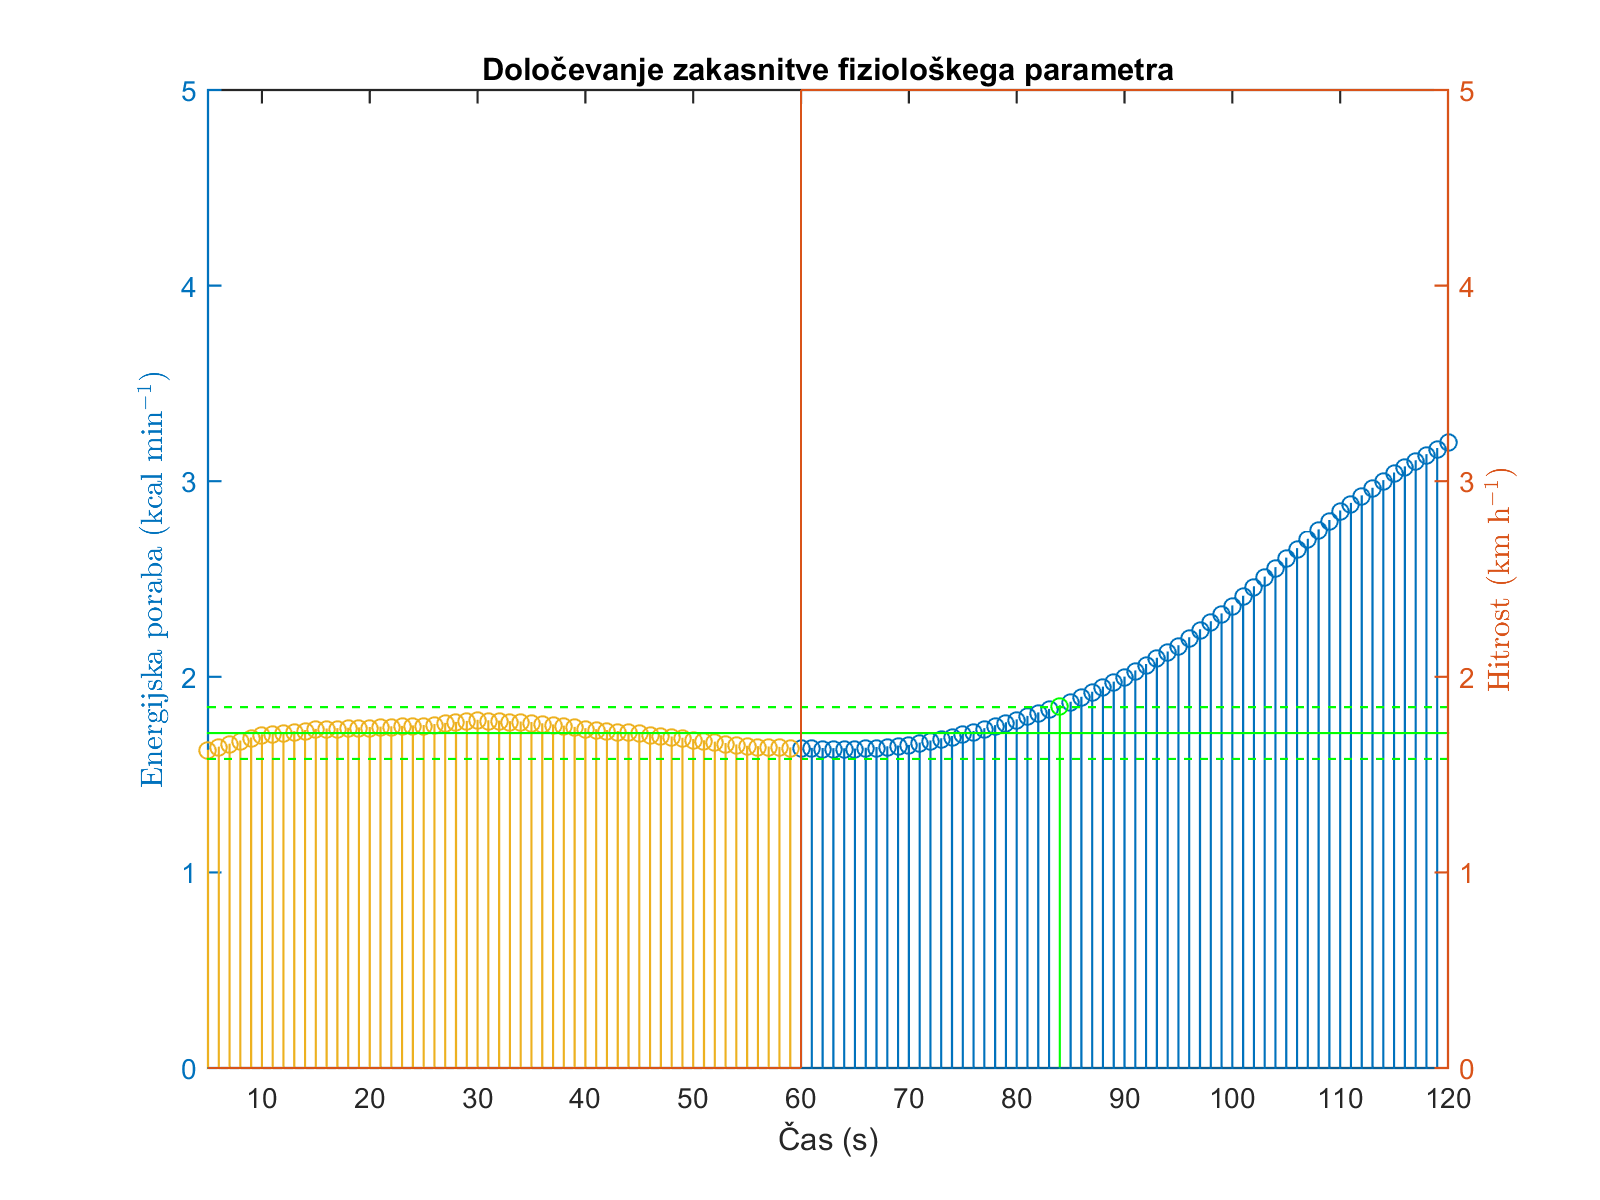
\includegraphics[width=\columnwidth]{./Slike/lag-estimation-1-eem.png}
		\caption{Zakasnitev za subjekt 1.}
		\label{fig:lag-estimation-1-eem}
	\end{subfigure}
	~
	\begin{subfigure}[t]{0.45\columnwidth}
		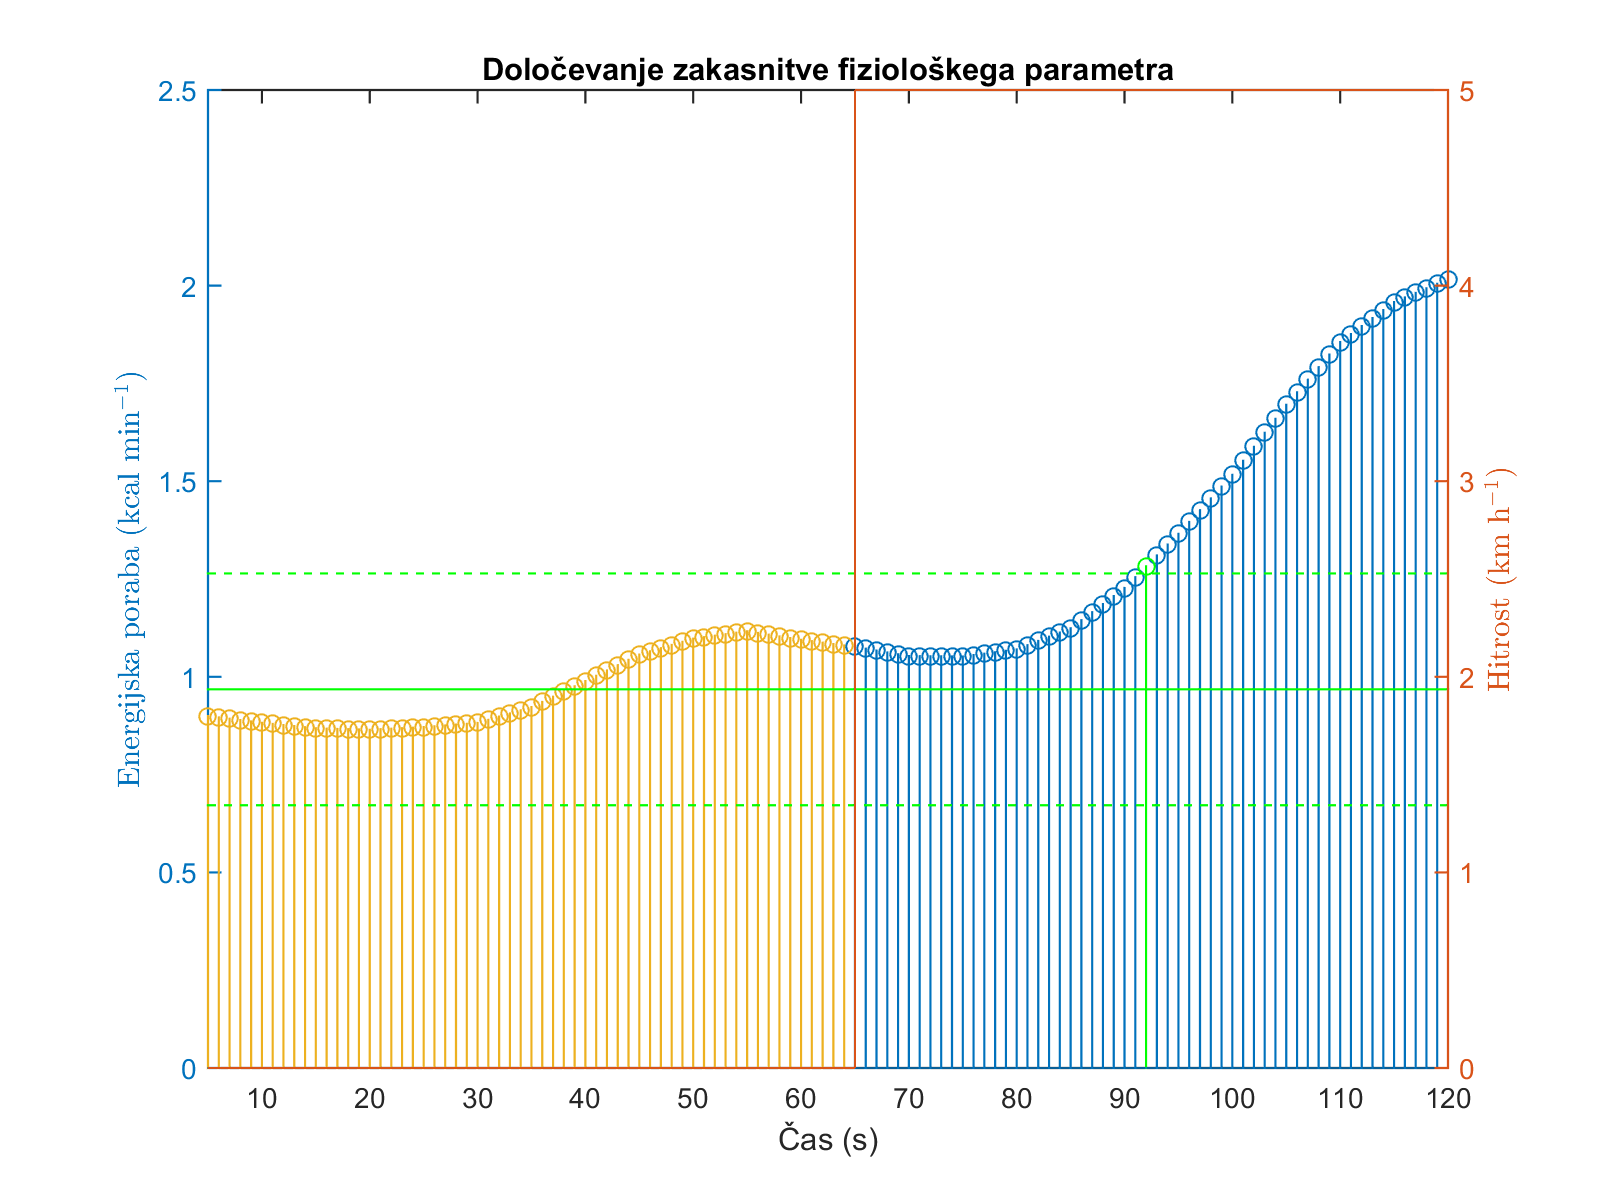
\includegraphics[width=\columnwidth]{./Slike/lag-estimation-2-eem.png}
		\caption{Zakasnitev za subjekt 2.}
		\label{fig:lag-estimation-2-eem}
	\end{subfigure}
	~
	\begin{subfigure}[t]{0.45\columnwidth}
		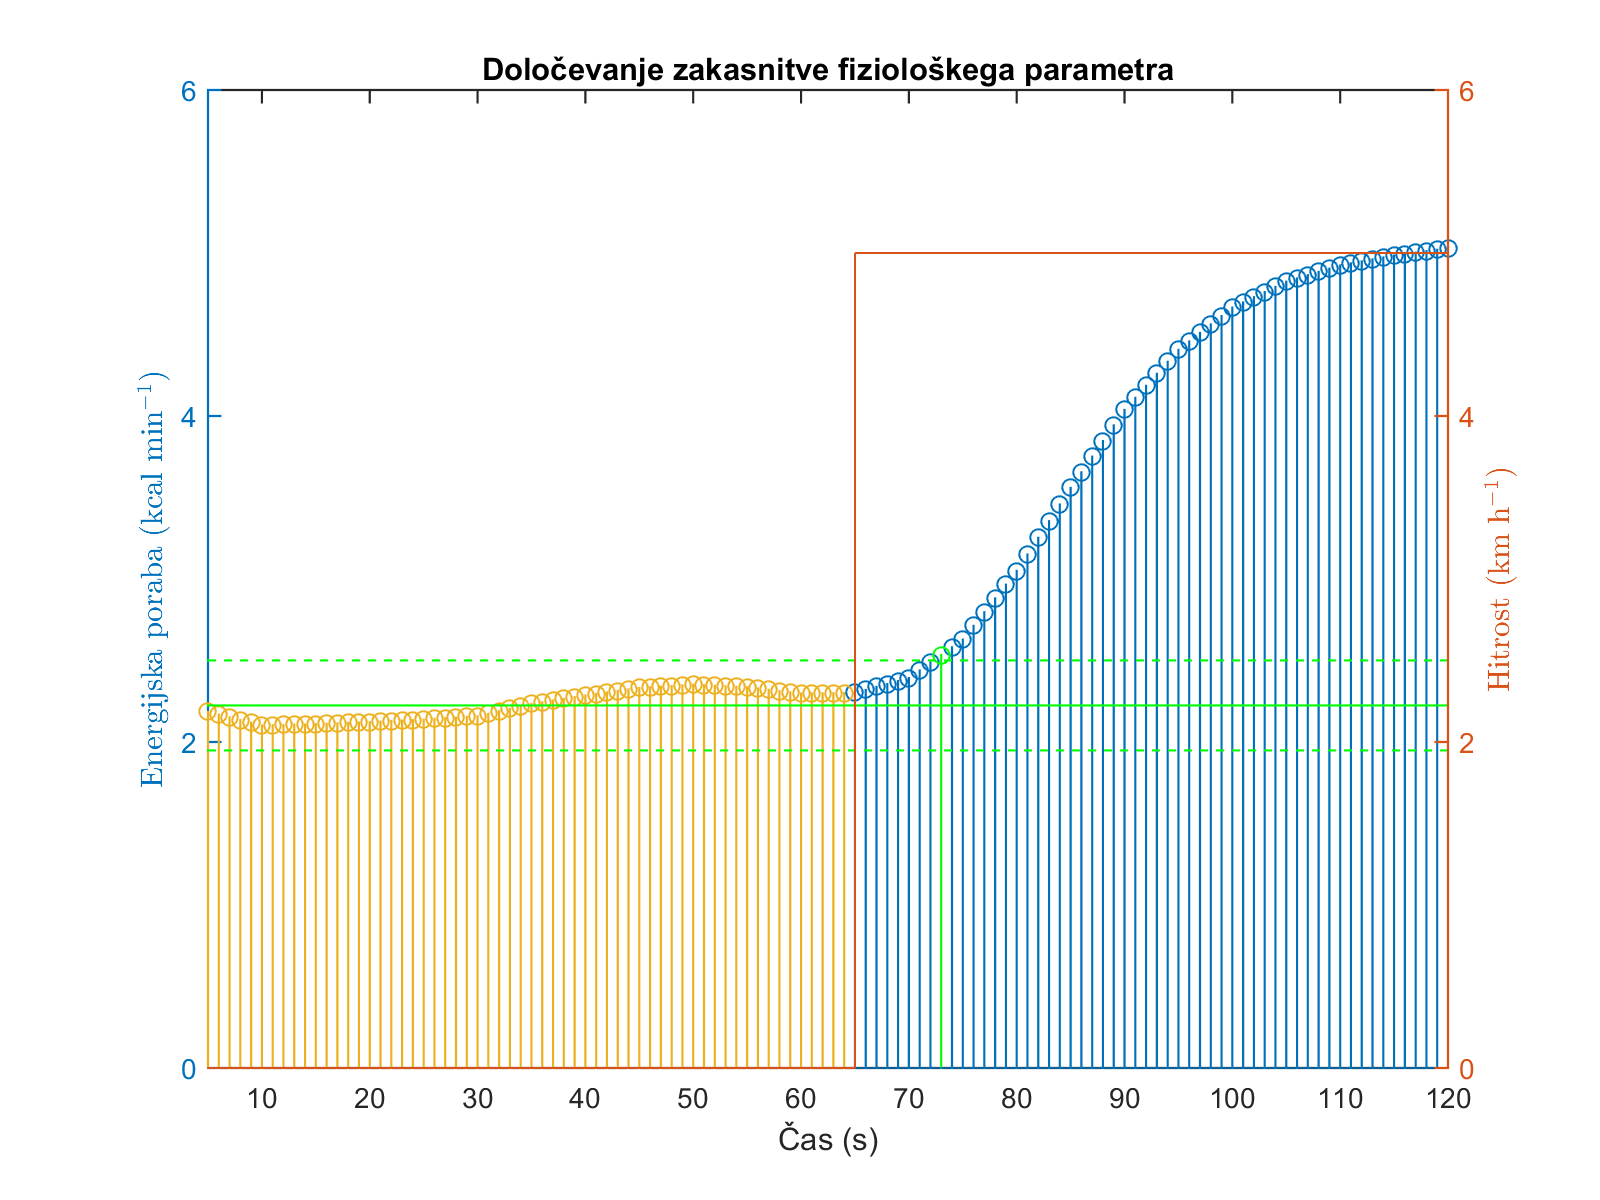
\includegraphics[width=\columnwidth]{./Slike/lag-estimation-3-eem.png}
		\caption{Zakasnitev za subjekt 3.}
		\label{fig:lag-estimation-3-eem}
	\end{subfigure}
	~
	\begin{subfigure}[t]{0.45\columnwidth}
		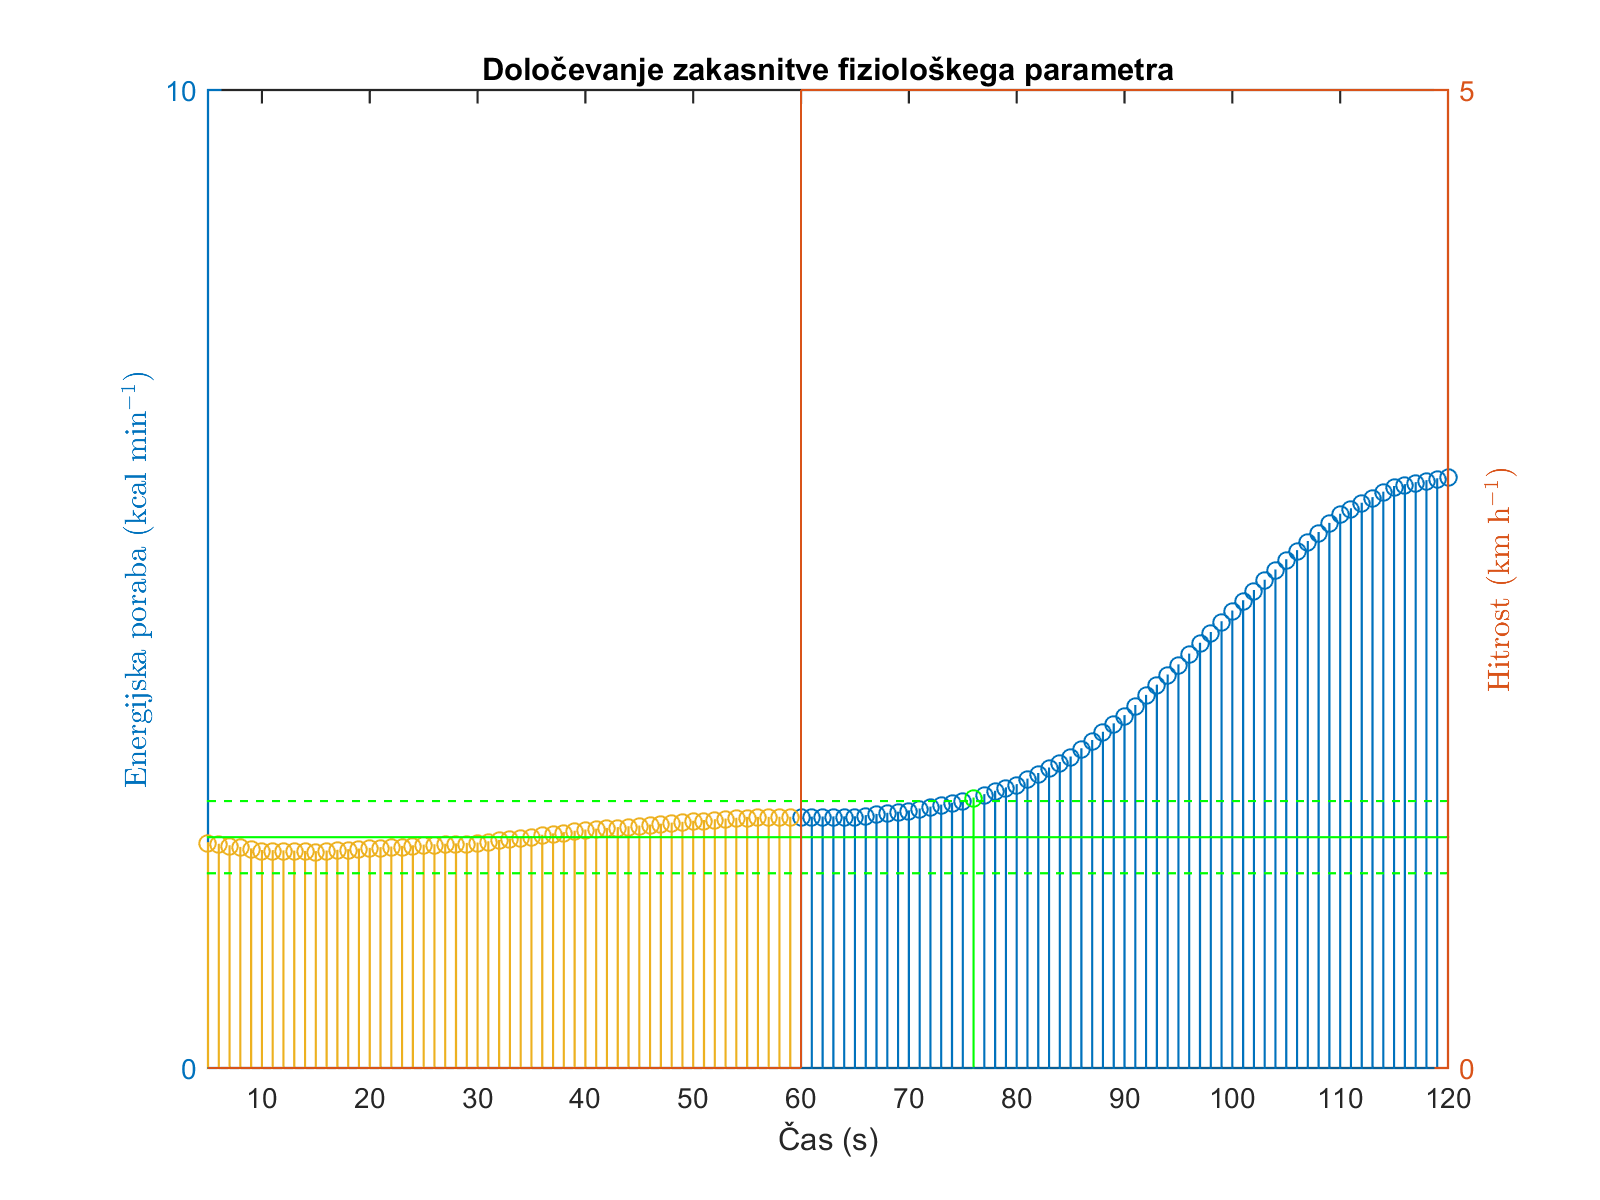
\includegraphics[width=\columnwidth]{./Slike/lag-estimation-4-eem.png}
		\caption{Zakasnitev za subjekt 4.}
		\label{fig:lag-estimation-4-eem}
	\end{subfigure}
	~
	\begin{subfigure}[t]{0.45\columnwidth}
		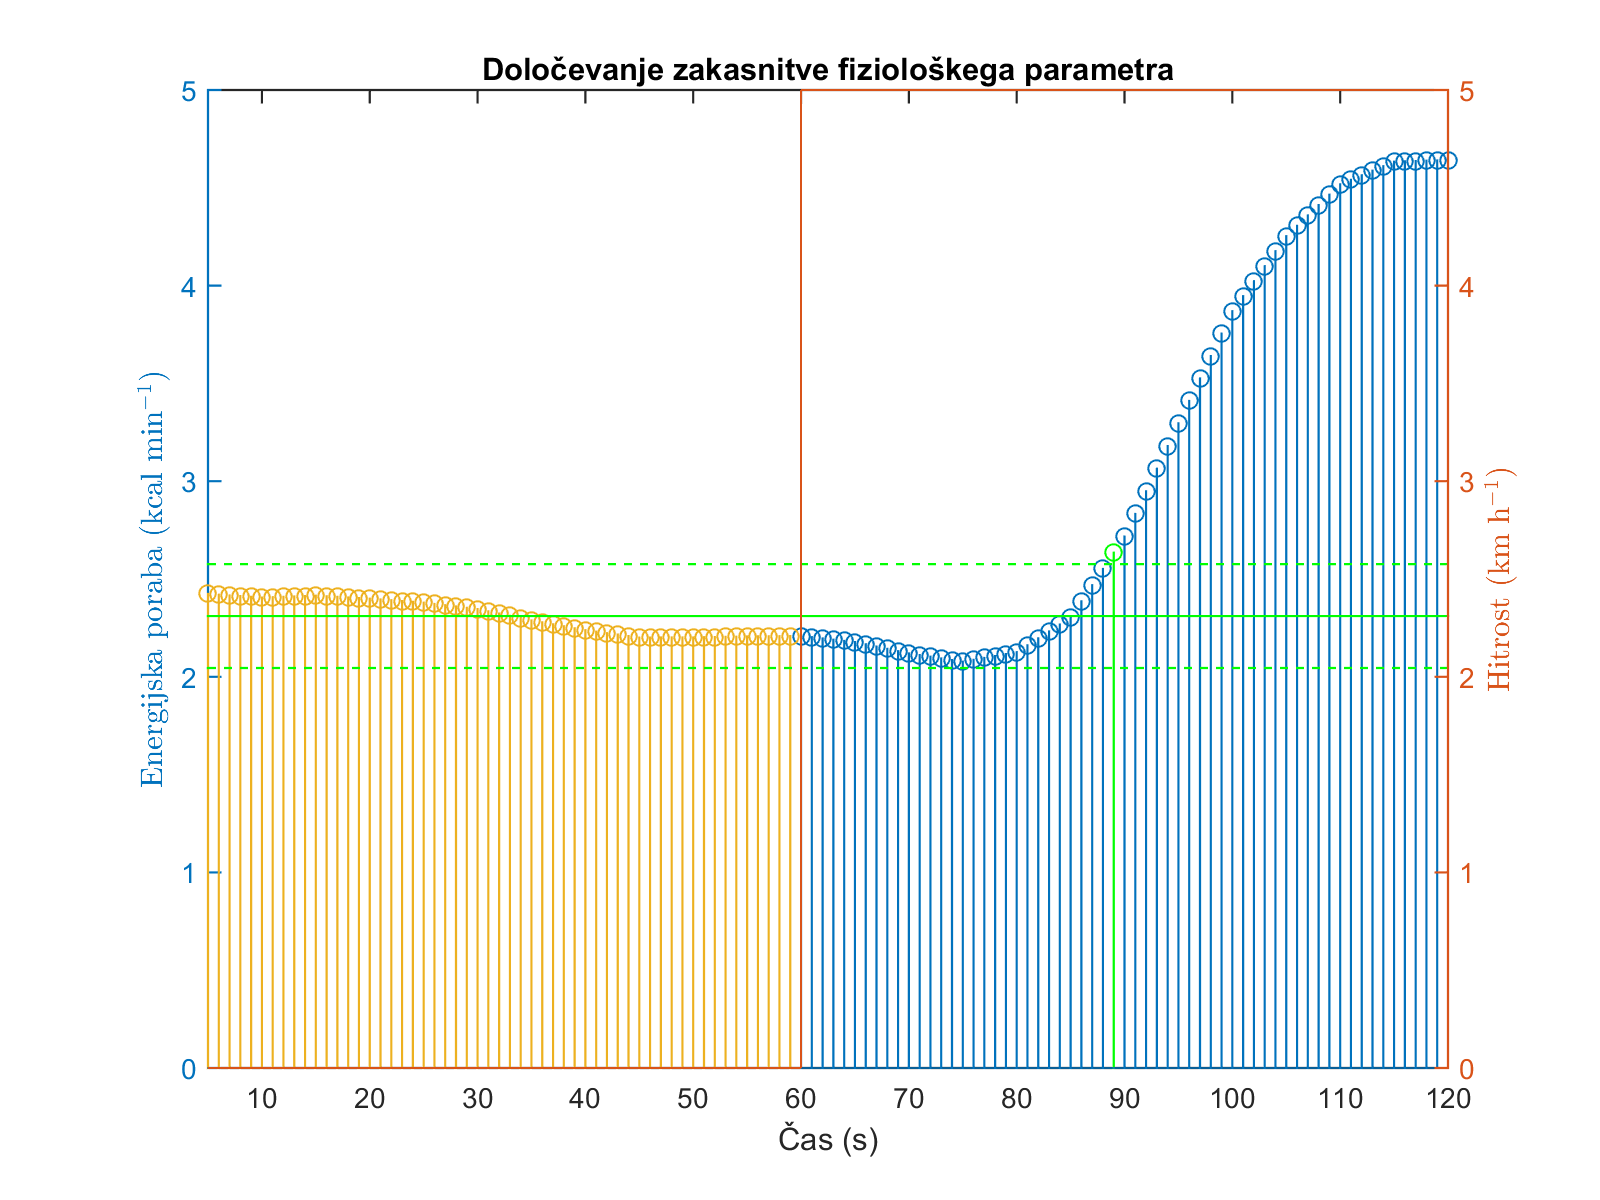
\includegraphics[width=\columnwidth]{./Slike/lag-estimation-5-eem.png}
		\caption{Zakasnitev za subjekt 5.}
		\label{fig:lag-estimation-5-eem}
	\end{subfigure}
	~
	\begin{subfigure}[t]{0.45\columnwidth}
		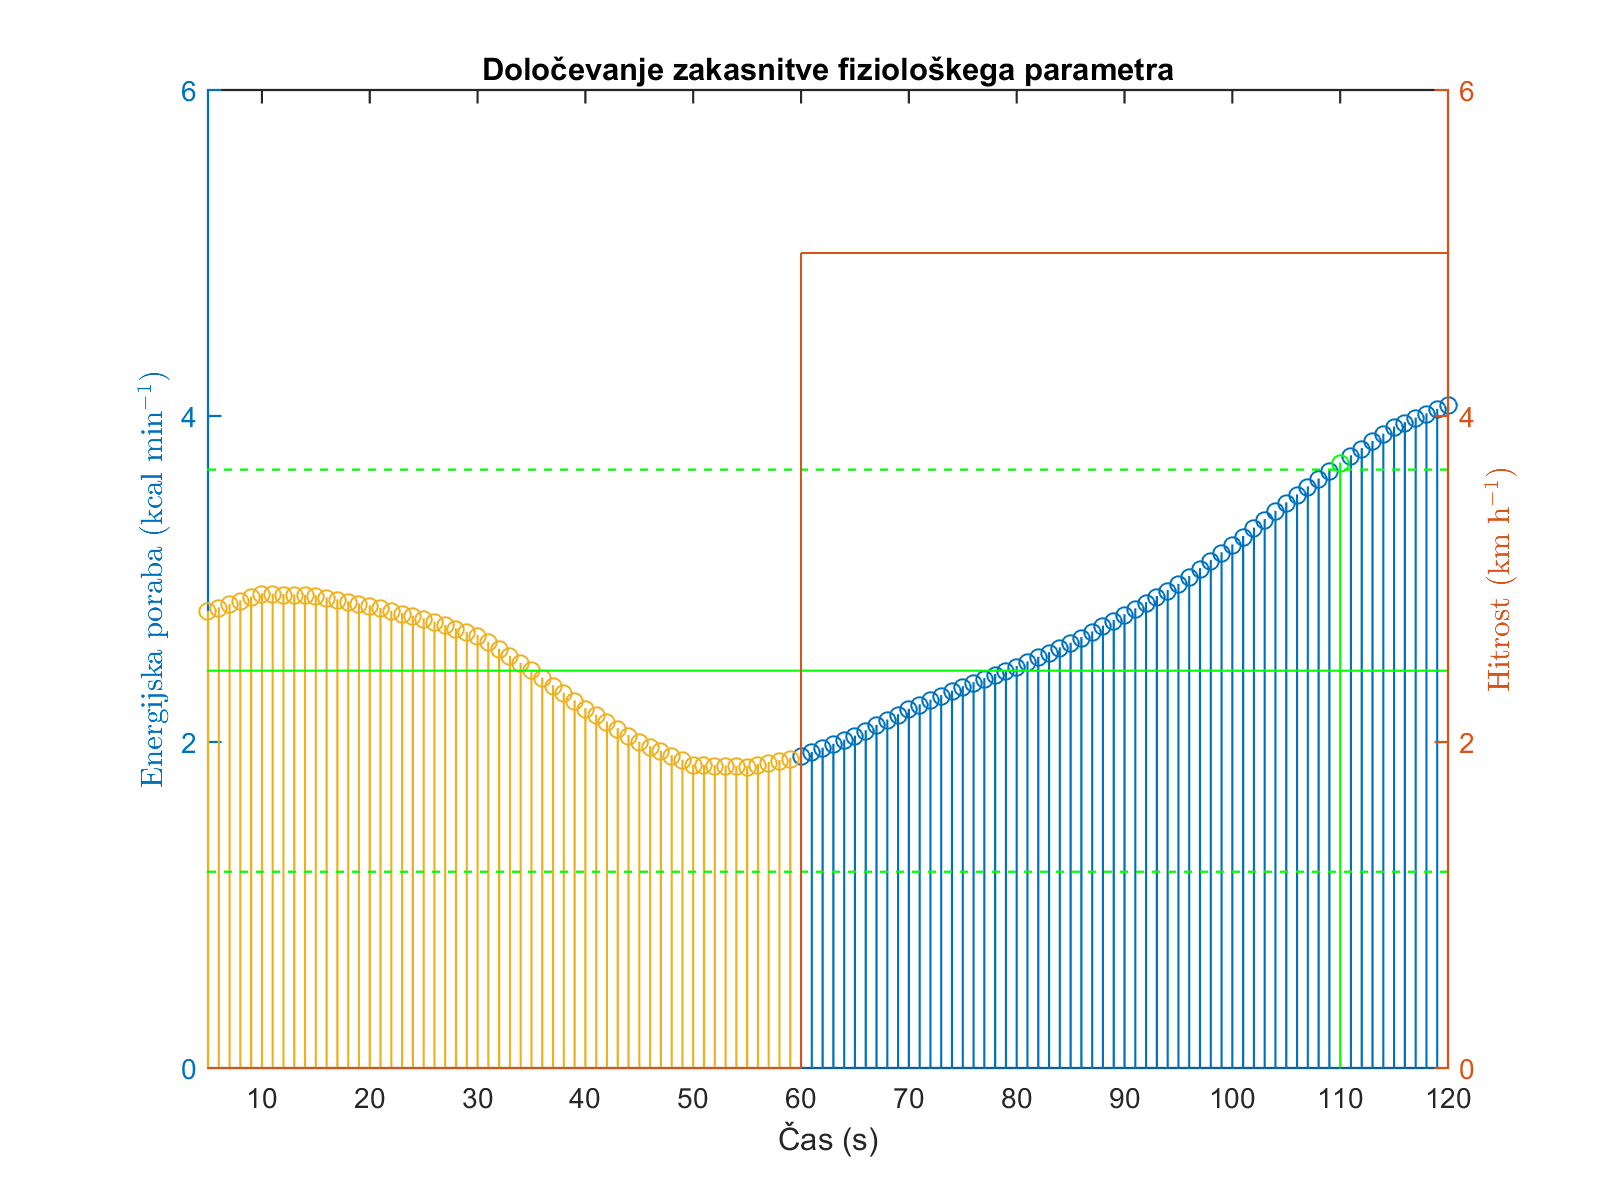
\includegraphics[width=\columnwidth]{./Slike/lag-estimation-6-eem.png}
		\caption{Zakasnitev za subjekt 6.}
		\label{fig:lag-estimation-6-eem}
	\end{subfigure}
	\caption{}
	\label{fig:lag-estimation-stage2}
\end{figure}










\subsection{Terenski eksperimenti}
Pri terenskih eksperimentih smo postopek z optičnim tokom in postopek s prostorskim tokom preverili še v realističnem okolju. Šest igralcev je igralo squash igro z dvema setoma. Tako smo pridobili podatke za 3 igre, ki so trajale \SI{16}{min} \SI{14}{min} in \SI{11}{min}. Postopki procesiranja in protokoli procesiranja so enaki kot v laboratorijskih eksperimentih 2. faze. 

\begin{figure}[htb]
	\centering
	\begin{subfigure}{0.45\columnwidth}
		%\includegraphics[width=\columnwidth]{./Slike/normal-sv-150.png}
		\caption{stranska slika}
	\end{subfigure}
	~
	\begin{subfigure}{0.45\columnwidth}
		%\includegraphics[width=\columnwidth]{./Slike/normal-bv-150.png}
		\caption{hrbtna slika}
	\end{subfigure}
	\caption{Hrbtna in stranska 150. slika RGB posnetkov iz prve serije.}
	\label{fig:primer-posnetka-teren}
\end{figure}

\paragraph{Pridobivanje podatkov.}
Igrišče smo snemali z dvema Microsoft Xbox Kinect V2 kamerama, ki sta bili oddaljeni ena od druge za približno \SI{2}{m}. Vsaka kamera je pokrivala svojo polovico igrišča. Razdalja od tal je znašala približno \SI{3}{m}. Kameri sta bili tako pozicionirani nad zaščitnim steklom. S tem nismo dobili odbojev laserskih žarkov, ki so namenjeni za pridobivanje globinske slike. Kot $\theta$ (rotacija okoli x osi) je bil približno $30\stopinj$ tako, da so kamere pokrivale prvo polovico igrišča do linije serviranja.

Pridobili smo barvne RGB in globinske DEPTH slike. Snemali smo v ločljivosti $512 \times 424$. Hitrost posnetkov je znašala \SI{30}{fps}. Kameri smo časovno sinhronizirali po NTP protokolu.

Fiziološke parametre smo pridobili s pomočjo prenosnega sistema za direktno ergospirometrijo tipa ``breath  by breath'' Cosmed K4B2. Frekvenca vzorčenja se je spreminjala, v povrečju pa je znašala \SI{0.5}{\hertz}. S testom smo pridobili podatke energijske porabe šestih različnih merjencev z oznakammi: SUBJ1, SUBJ2, SUBJ7, SUBJ8, SUBJ9 in SUBJ10.

\paragraph{Protokol izvajanja meritev.}
Posamezno igro smo pričeli s 5 minutnim ogrevalnim tekom. Sledilo je igranje na dva seta do 10 dobljenih točk z upoštevanjem dveh točk razlike. Med setoma so igralci počivali 2 minute. Ogrevanja in počivanja s kamerami nismo merili. Seta posamezne igre smo združili v en posnetek.

\chapter{Rezultati}\label{sec:rezultati}
All energy consumption and heart rate models were validated on previously described test samples. For comparison between the different models we have chosen validation measures: correlation coefficient (CORR), relative absolute error (RAE) and root relative square error (RRSE) \cite{witten2005data}. We have also added ratio between number of support vectors and number of training data (nSV). The higher the value of the CORR the better, with RAE, RRSE and nSV is other way around.

Models were also evaluated with cross testing. This testing was done only by the type of input data (side-view or back-view). \textit{sv} models, that were made with learning samples from side-view camera were first tested with testing samples from side-view camera and then with back-view camera. Hereafter tests with input data from side-view camera are marked with \textit{sv} in brackets and tests with input data from back-view camera are marked with \textit{bv} in brackets.


















\section{Eksperimenti 1. faze}


\subsection{Preliminarni testi}

\subsubsection{Optimizacija HOOF deskriptorjev}\label{sec:rezultati-optimizacija-hoof}
Parameter $N_{HOOF}$ smo določili na podlagi rezultatov evaluacije v tabeli \ref{tab:nhoof} in grafov korelacije med referenčnimi podatki in predikcijo \ref{fig:corr-hoof}.

V tabeli \ref{tab:nhoof} lahko vidimo, da se povečevanjem števila stolpcev rezultati bistveno ne razlikujejo. Najbojlši rezultate nam sicer daje $120$ stolpcev, vendar pa smo za potrebe naše metode uporabili $N_{HOOF}=60$, ki je ravno tako dal zadovoljive rezultate. S takim številom smo zagotovili dobro delovanje glede na minimalno vrednost, še vseeno pa ne gre za tako veliko število, ko bi do izraza prišle amplitude šumnih vektorjev.

\begin{table}[!htbp]
	\centering
	\begin{tabular}{S[table-format=2.0] S[table-format=1.3] S[table-format=1.3] S[table-format=1.3] S[table-format=2.2]}
		\toprule
		\thead{$\mathbf{N_{HOOF}}$} & \thead{$\mathbf{r}$} & \thead{RAE} & \thead{RRSE} & \thead{nSV [\%]}\\
		\midrule%nSV
		30 & 0.978 & 0.296 & 0.304 & \boldentry{2}{2}{62.81}\\%18089
		\boldentry{2}{0}{60} & 0.980 & 0.277 & 0.289 & 81.21\\%23388
		120 & \boldentry{1}{2}{0.983} & \boldentry{1}{3}{0.261} & \boldentry{1}{3}{0.273} & 74.39\\%21424
		160 & 0.982 & 0.272 & 0.284 & 71.68\\%20644
		\bottomrule
	\end{tabular}
	\caption[Rezultati evaluacije modelov z različnim $N_{HOOF}$]{Rezultati evaluacije modelov z različnim številom stolpcev $N_{HOOF}$ HOOF deskriptorja. Optimalni rezultati so odebeljeni. Kljub dobrim rezultatom modela z $N_{HOOF}=120$ smo izbrali $N_{HOOF}=60$, ker nanj šum manj vpliva.}
	\label{tab:nhoof}
\end{table}

\begin{figure}[!htbp]
	\centering
	\begin{subfigure}[t]{0.45\columnwidth}
		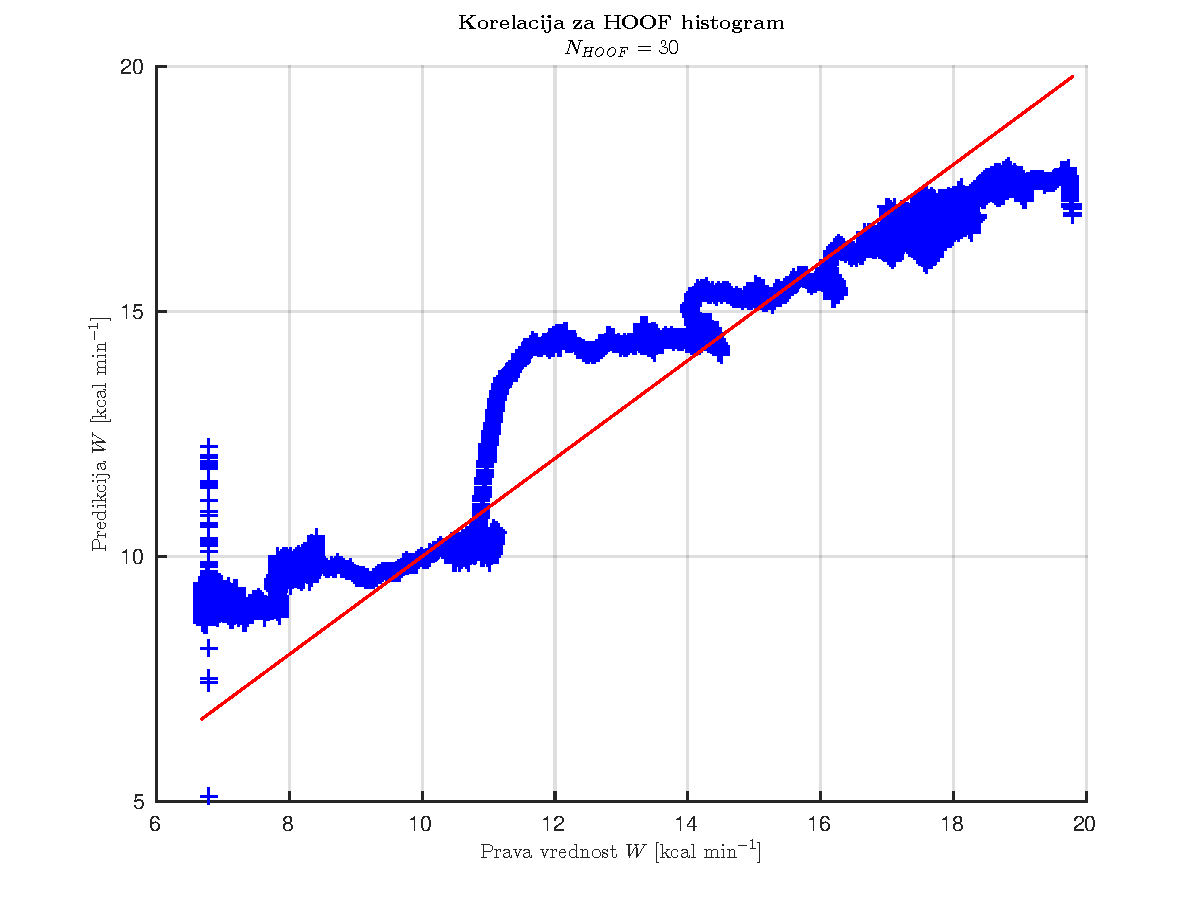
\includegraphics[width=\columnwidth]{corr-hoof-30-sl}
		\caption{Korelacija $N_{HOOF}=30$.}
		\label{fig:corr-hoof-30}
	\end{subfigure}
	~
	\begin{subfigure}[t]{0.45\columnwidth}
		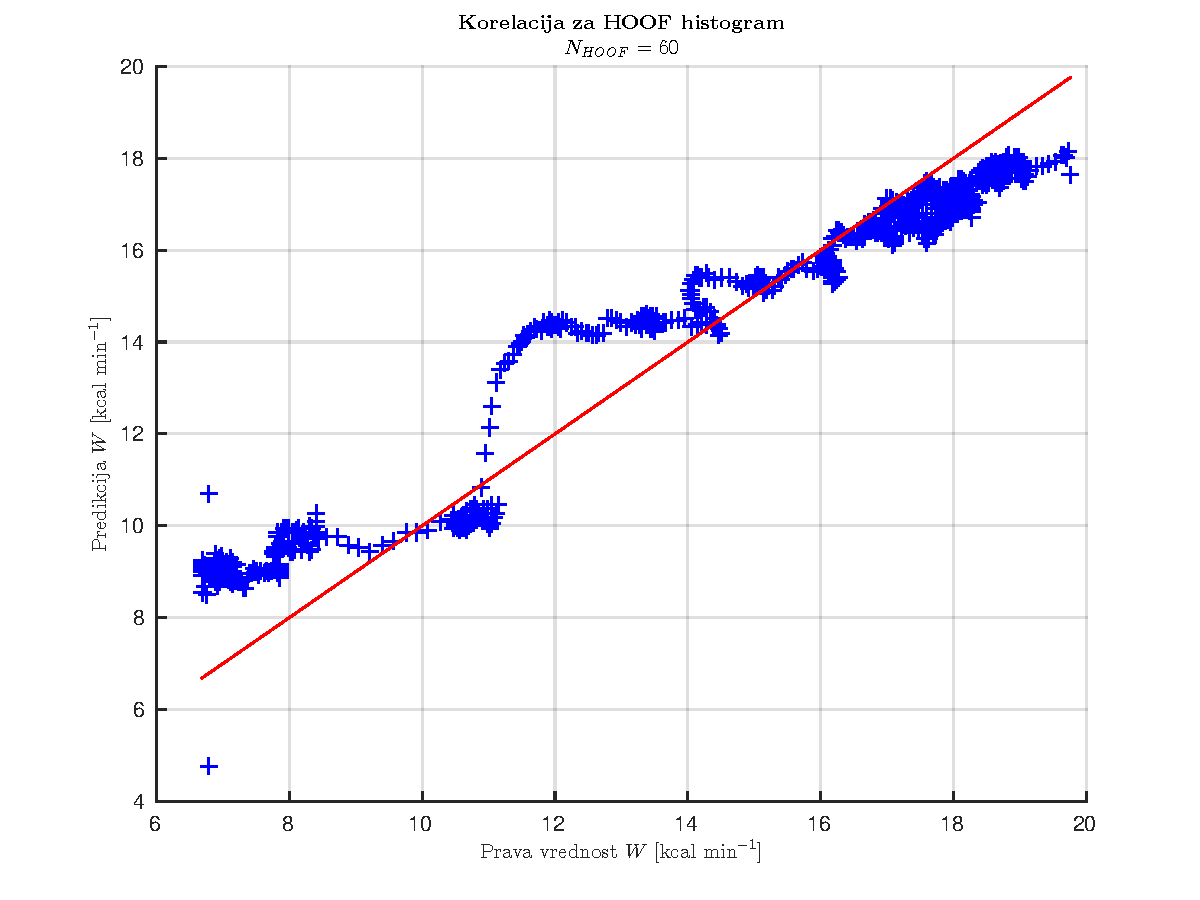
\includegraphics[width=\columnwidth]{corr-hoof-60-sl}
		\caption{Korelacija $N_{HOOF}=60$.}
		\label{fig:corr-hoof-60}
	\end{subfigure}
	~
	\begin{subfigure}[b]{0.45\columnwidth}
		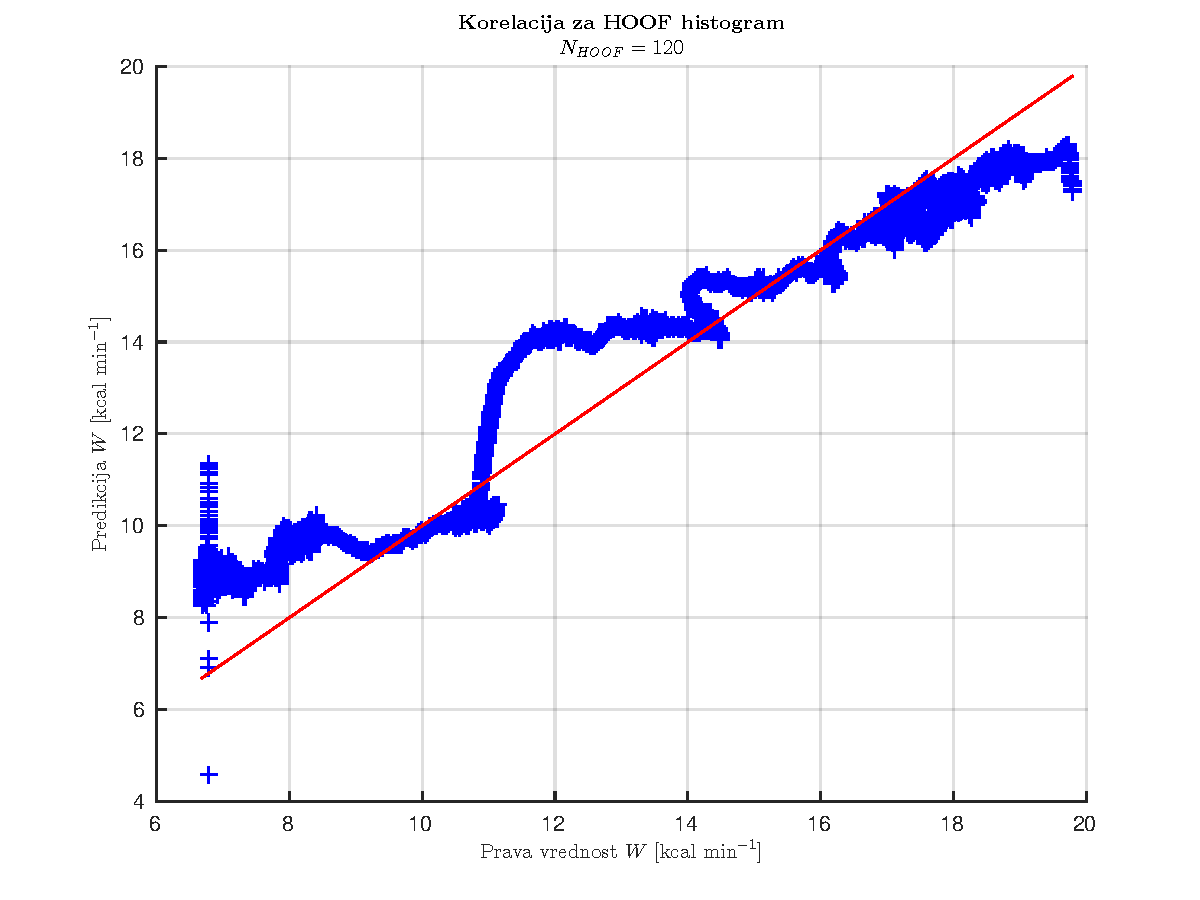
\includegraphics[width=\columnwidth]{corr-hoof-120-sl}
		\caption{Korelacija $N_{HOOF}=120$.}
		\label{fig:corr-hoof-120}
	\end{subfigure}
	~
	\begin{subfigure}[b]{0.45\columnwidth}
		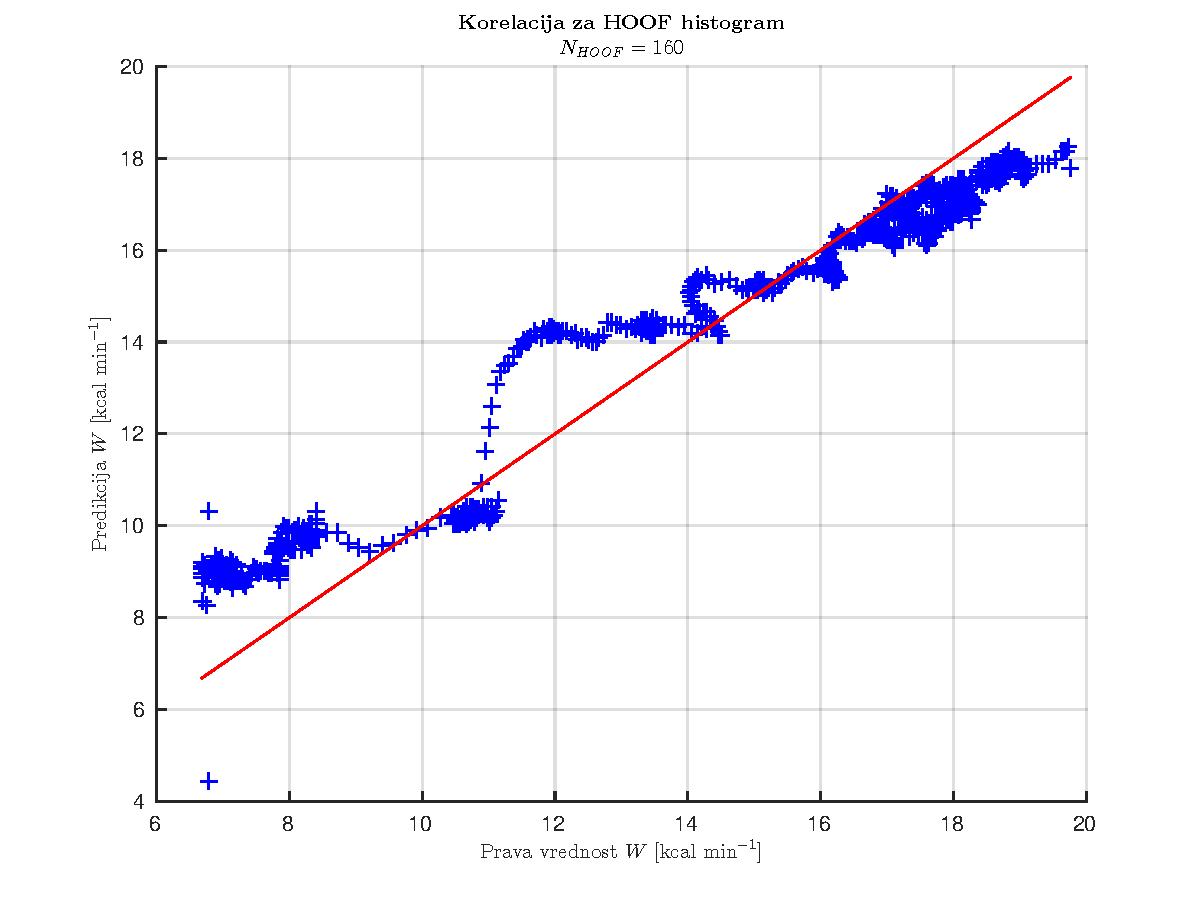
\includegraphics[width=\columnwidth]{corr-hoof-160-sl}
		\caption{Korelacija $N_{HOOF}=160$.}
		\label{fig:corr-hoof-160}
	\end{subfigure}
	\caption[Grafi korelacij modelov z različnim $N_{HOOF}$]{Grafi korelacij modelov z različnim številom stolpcev $N_{HOOF}$ HOOF deskriptorja. Rezultati so si zelo podobni.}
	\label{fig:corr-hoof}
\end{figure}












\subsubsection{Optimizacija HAFA deskriptorjev}\label{sec:rezultati-optimizacija-hafa}
Parameter $N_{HAFA}$ smo določili na podlagi rezultatov evaluacije v tabeli \ref{tab:nhafa} in grafov korelacije med referenčnimi podatki in predikcijo \ref{fig:corr-hafa}.

\begin{table}[!htbp]
	\centering
	\begin{tabular}{S[table-format=2.0] S[table-format=1.3] S[table-format=1.3] S[table-format=1.3] S[table-format=2.2]}
		\toprule
		\thead{$\mathbf{N_{HAFA}}$} & \thead{$\mathbf{r}$} & \thead{RAE} & \thead{RRSE} & \thead{nSV [\%]}\\
		\midrule%nSV
		30 & 0.984 & 0.213 & 0.231 & 62.08 \\%17879/28799
		\boldentry{2}{0}{60} & \boldentry{1}{3}{0.984} & \boldentry{1}{3}{0.211} & \boldentry{1}{3}{0.228} & \boldentry{2}{2}{62.60} \\%18028
		120 & 0.984 & 0.211 & 0.228 & 62.63 \\%18037
		160 & 0.984 & 0.211 & 0.228 & 62.63 \\%18037
		\bottomrule
	\end{tabular}
	\caption[Rezultati evaluacije modelov z različnim $N_{HAFA}$]{Rezultati evaluacije modelov z različnim številom stolpcev $N_{HAFA}$ HAFA deskriptorja. Optimalni rezultati so odebeljeni.}
	\label{tab:nhafa}
\end{table}

V tabeli \ref{tab:nhafa} lahko vidimo, da so rezultati praktično enaki. Za našo metodo smo izbrali $N_{HAFA}=60$, kar v grobem predstavlja $60$ različnih hitrosti z maksimalno amplitudo \SI{60}{px.f^{-1}}.

\begin{figure}[!htbp]
	\centering
	\begin{subfigure}[t]{0.45\columnwidth}
		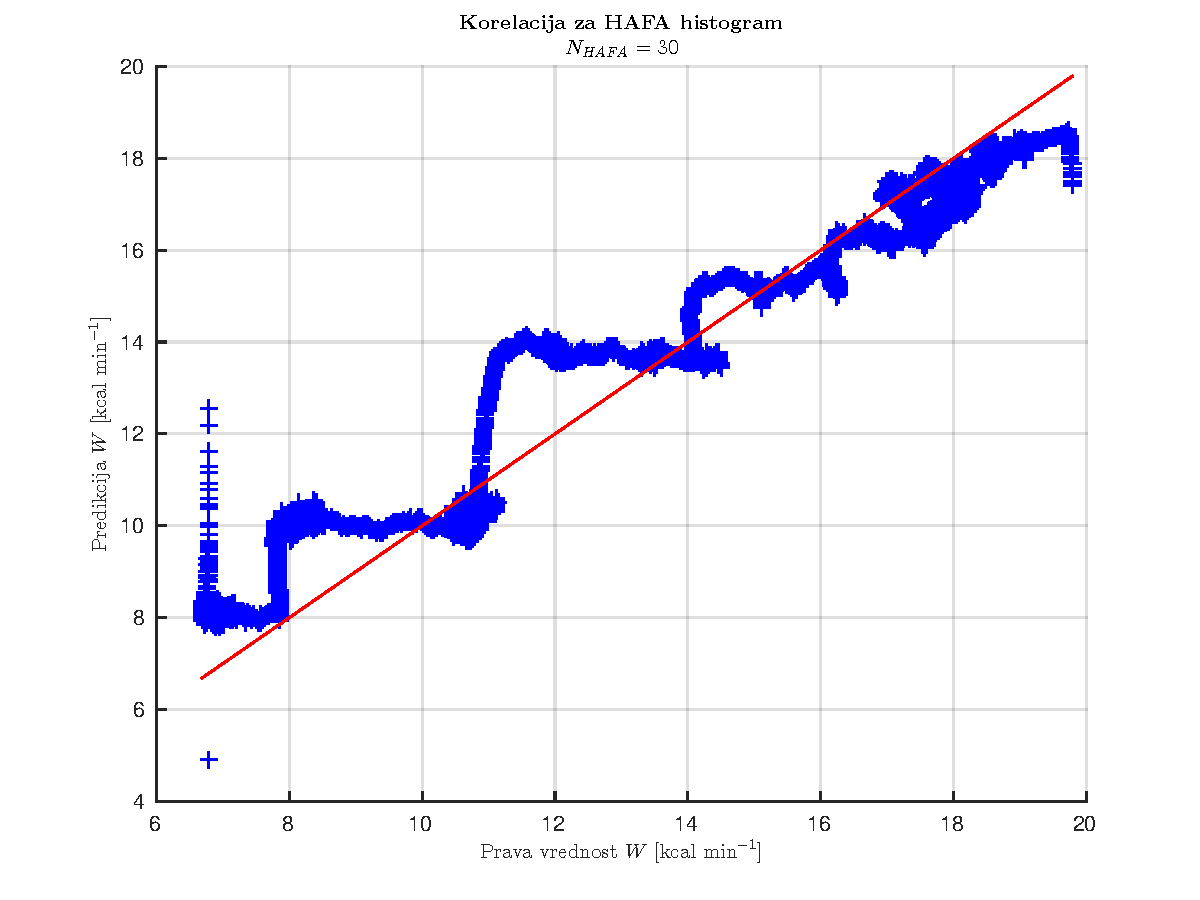
\includegraphics[width=\columnwidth]{corr-hafa-30-sl}
		\caption{Korelacija $N_{HAFA}=30$.}
		\label{fig:corr-hafa-30}
	\end{subfigure}
	~
	\begin{subfigure}[t]{0.45\columnwidth}
		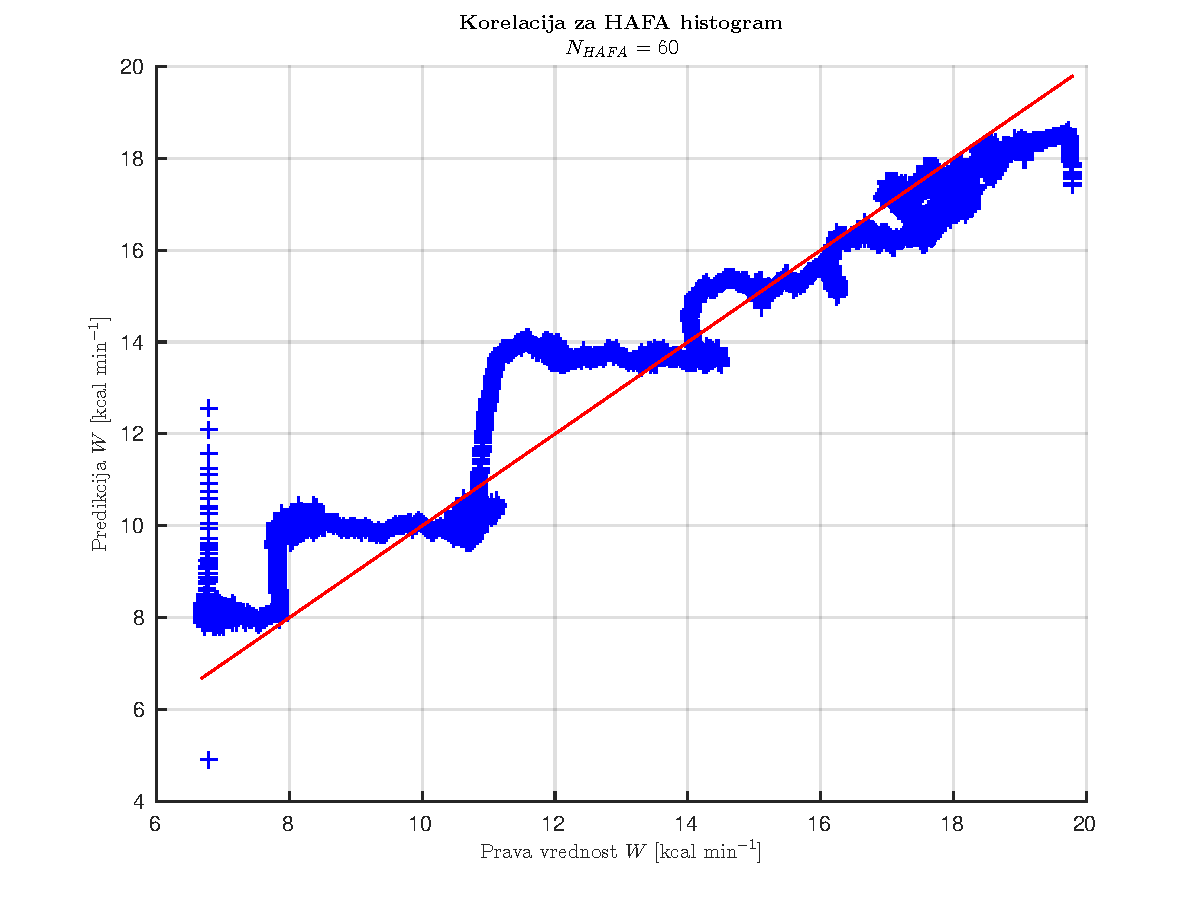
\includegraphics[width=\columnwidth]{corr-hafa-60-sl}
		\caption{Korelacija $N_{HAFA}=60$.}
		\label{fig:corr-hafa-60}
	\end{subfigure}
	~
	\begin{subfigure}[b]{0.45\columnwidth}
		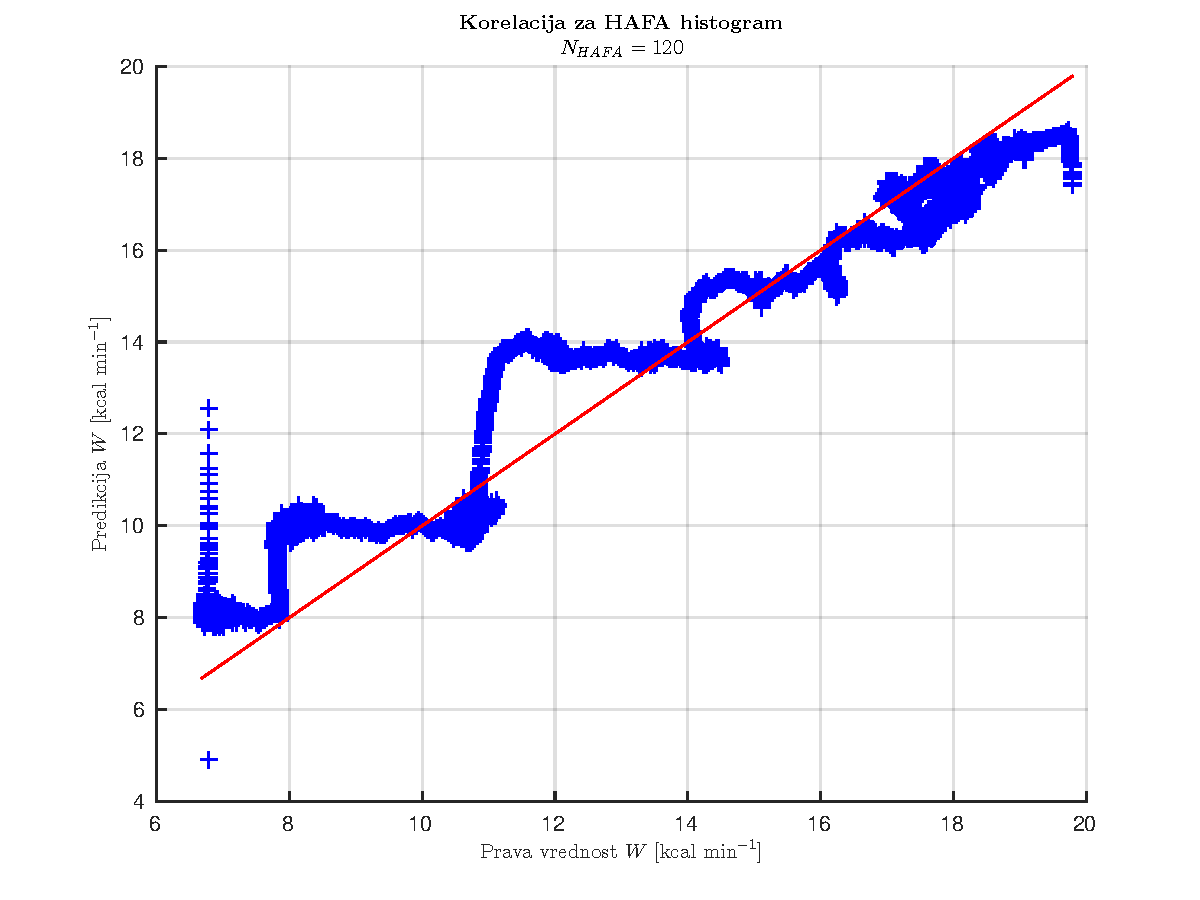
\includegraphics[width=\columnwidth]{corr-hafa-120-sl}
		\caption{Korelacija $N_{HAFA}=120$.}
		\label{fig:corr-hafa-120}
	\end{subfigure}
	~
	\begin{subfigure}[b]{0.45\columnwidth}
		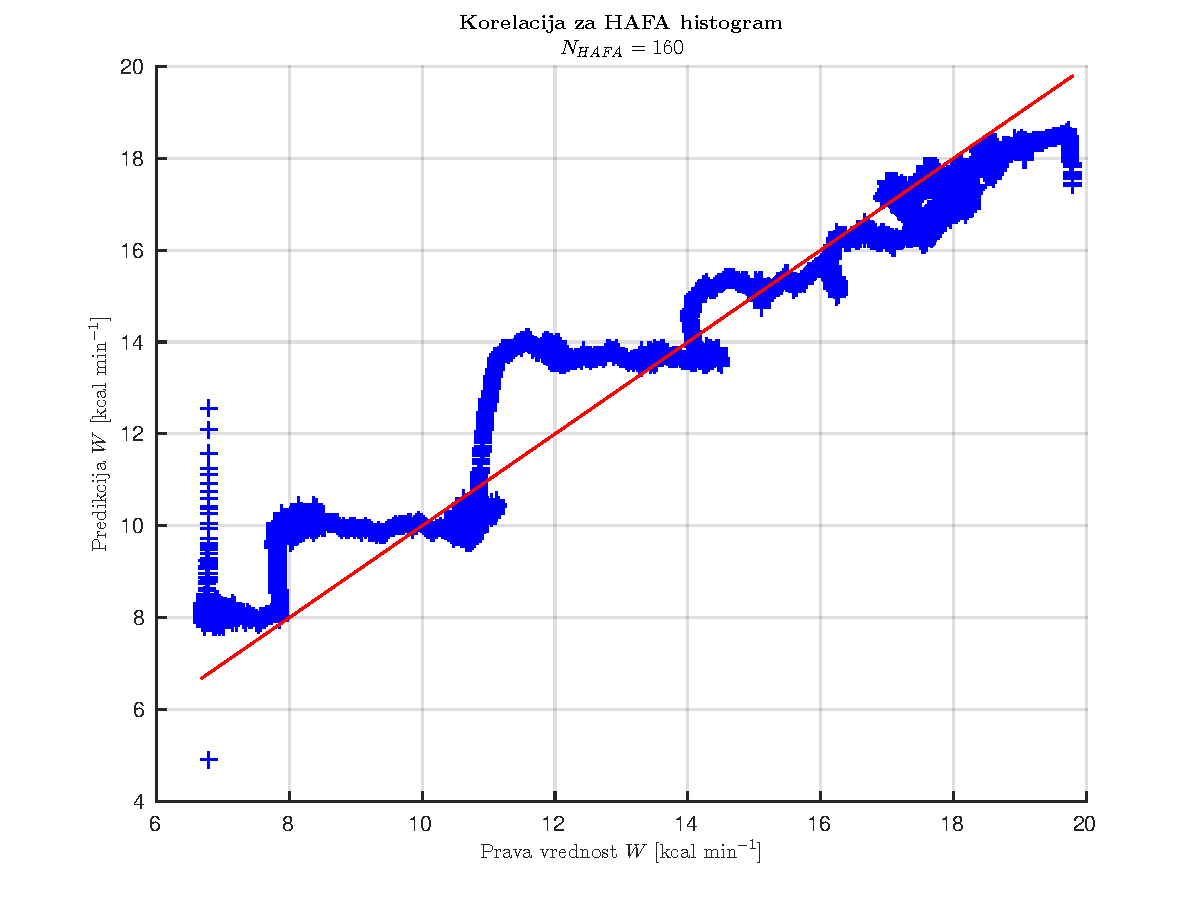
\includegraphics[width=\columnwidth]{corr-hafa-160-sl}
		\caption{Korelacija $N_{HAFA}=160$.}
		\label{fig:corr-hafa-160}
	\end{subfigure}
	\caption[Grafi korelacij modelov z različnim $N_{HAFA}$]{Grafi korelacij modelov z različnim številom stolpcev $N_{HAFA}$ HAFA deskriptorja. Rezultati so si zelo podobni.}
	\label{fig:corr-hafa}
\end{figure}











\subsubsection{Razširitev HOOF deskriptorja}\label{sec:rezultati-razsiritev-hoof}

\begin{table}[!htbp]
	\centering
	\begin{tabular}{l S[table-format=1.3] S[table-format=1.3] S[table-format=1.3] S[table-format=2.2]}
		\toprule
		\textbf{Deskriptor} & \thead{$\mathbf{r}$} & \thead{RAE} & \thead{RRSE} & \thead{nSV [\%]}\\
		\midrule%nSV
		HOOF & 0.992 & 0.336 & 0.317 & \boldentry{2}{2}{82.34} \\%2187/2656
		\textbf{HOOF-HAFA} & \boldentry{1}{3}{0.991} & \boldentry{1}{3}{0.157} & \boldentry{1}{3}{0.205} & 89.53 \\%2378
		\bottomrule
	\end{tabular}
	\caption[Rezultati evaluacije modelov z različnim deskriptorjem]{Rezultati evaluacije modelov z različnim deskriptorjem. Optimalni rezultati so odebeljeni. Vidimo lahko, da se bolje odnese razširjeni deskriptor HOOF-HAFA, čeprav model uporablja več podpornih vektorjev. }
	\label{tab:izbira}
\end{table}



\begin{figure}[!htbp]
	\centering
	\begin{subfigure}[t]{0.45\columnwidth}
		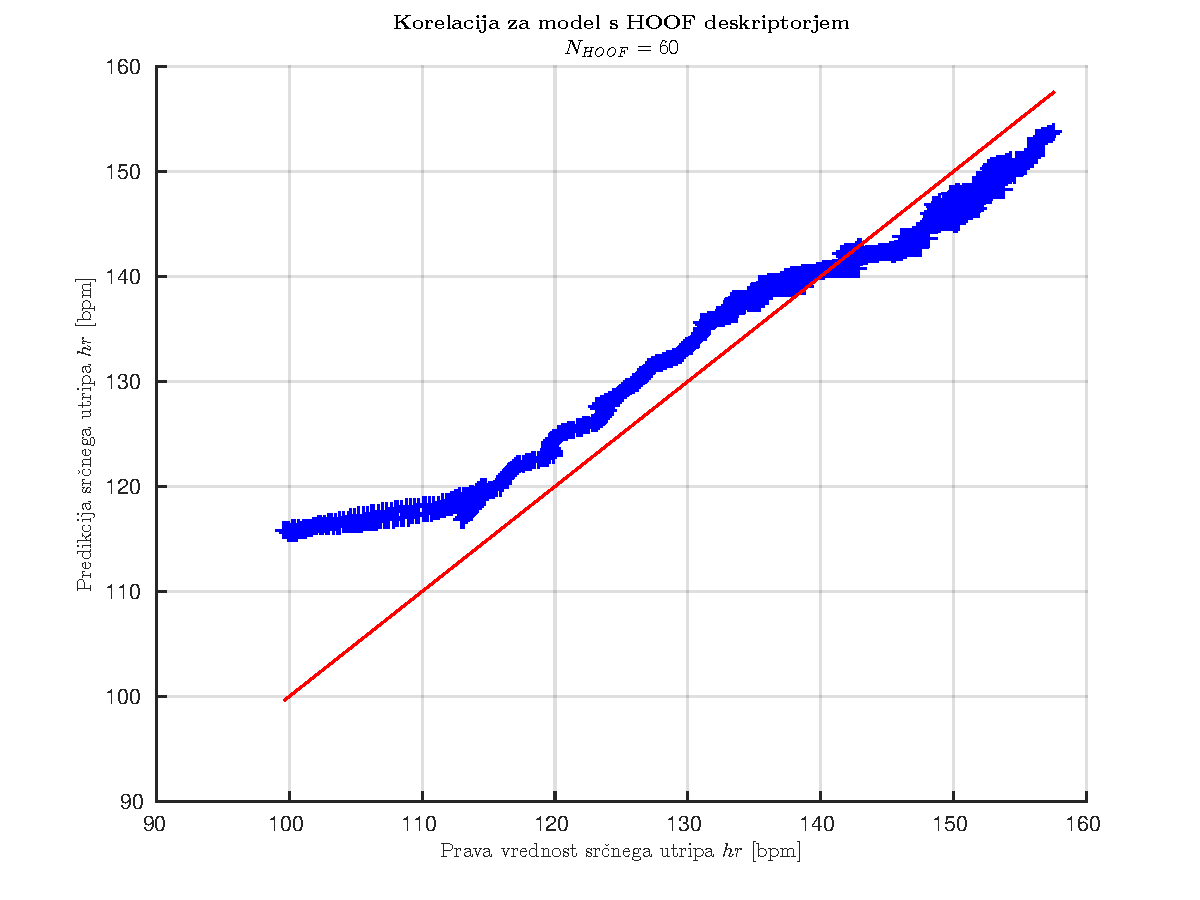
\includegraphics[width=\columnwidth]{corr-hoof-sl}
		\caption{Korelacija $N_{HOOF}=60$.}
		\label{fig:izbira-hoof}
	\end{subfigure}
	~
	\begin{subfigure}[t]{0.45\columnwidth}
		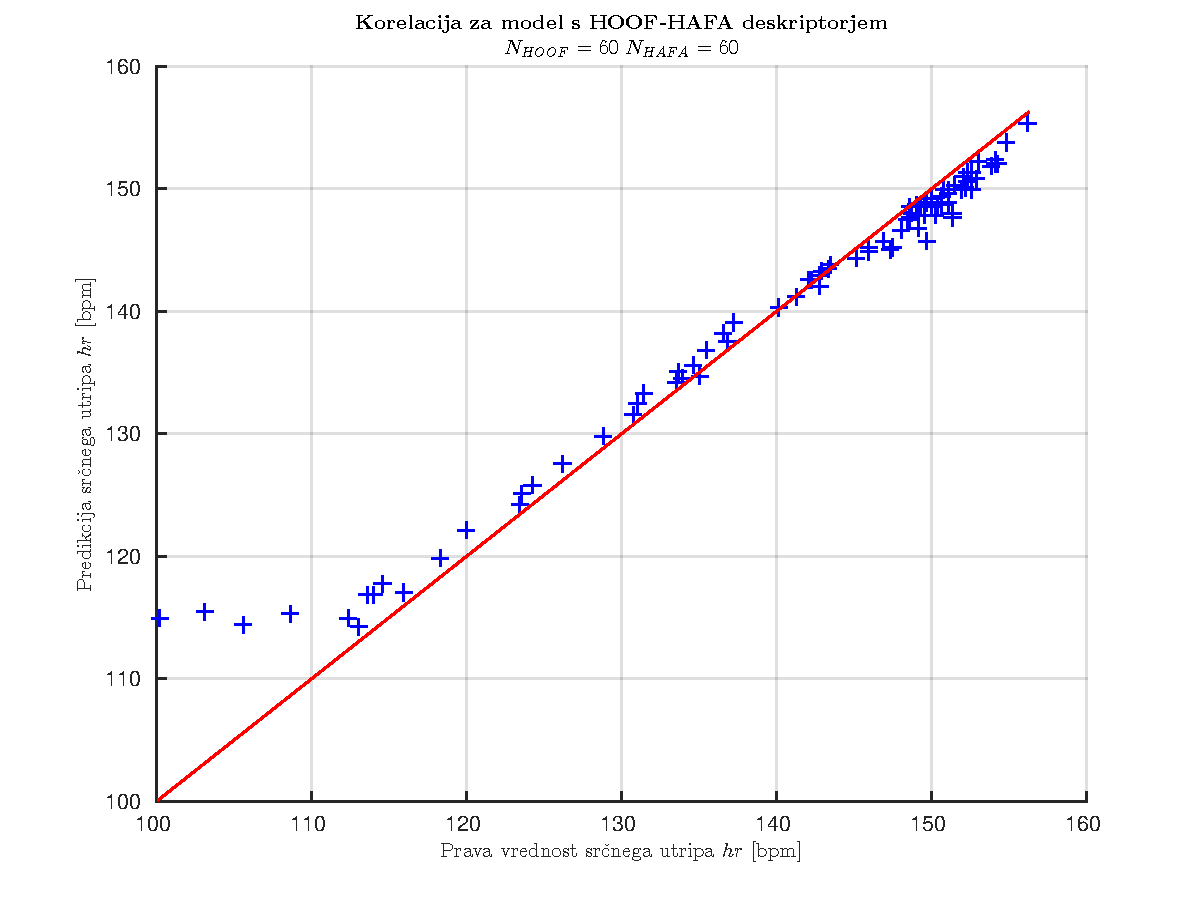
\includegraphics[width=\columnwidth]{corr-hoof-hafa-sl}
		\caption{Korelacija $N_{HOOF}=60$,\\$N_{HAFA}=60$.}
		\label{fig:izbira-hoofhafa}
	\end{subfigure}
	\caption[Primerjava modelov s HOOF in HOOF-HAFA deskriptorji]{Primerjava grafov korelacij modelov z različnimi deskriptorji. Model \subref{fig:izbira-hoof}) smo naučili s HOOF deskriptorjem. Model \subref{fig:izbira-hoofhafa}) smo naučili s HOOF in HAFA deskriptorjem. Posamezen vzorec je tako vseboval $120$ značilk. Pri primerjavi korelacije lahko opazimo vidno razliko. Model \subref{fig:izbira-hoofhafa}) dokazuje, da je razširjeni deskriptor boljši.}
	\label{fig:izbira}
\end{figure}




















\subsubsection{Sledilniki za optični tok} \label{sec:rezultati-sledilnikov-za-opticni-tok}


Rezultati testiranja so prikazani v tabeli \ref{tab:region-overlap}. Za izbrane sledilnike smo določili povprečje prekrivanja področja za posamezen posnetek. V tretjem stolpcu je predstavljeno povprečje prekrivanja glede na oba posnetka. Najboljši rezultati so odebeljeni. Po tabeli \ref{tab:region-overlap} se za posnetek \textit{handball1} najbolje izkaže CORR sledilnik. Za posnetek \textit{handball2} smo dobili najboljše rezultate pri sledilniku OPENCV-TLD. V povprečju se najbolje izkaže sledilnik CORR.




\begin{table}[!htbp]
	\centering
	\begin{tabular}{l S[table-format=1.3] S[table-format=1.3] S[table-format=1.3]}
		\toprule
		\textbf{Sledilnik} & \thead{$\mathbf{\Phi(\mathrm{handball1})}$} & \thead{$\mathbf{\Phi(\mathrm{handball2})}$} & \thead{$\mathbf{\overline{\Phi}}$}  \\
		\midrule%nSV
		NEBEHAY-TLD & 0.035 & 0.130 & 0.083 \\
		CCV-TLD & 0.117 & 0 & 0.117 \\
		OPENCV-TLD & 0.002 & \boldentry{1}{3}{0.178} & 0.09 \\
		CORR & \boldentry{1}{3}{0.214} & 0.160 & \boldentry{1}{3}{0.187} \\
		\textbf{KCF} & {0.161} & {0.166} & {0.164} \\
		\bottomrule
	\end{tabular}
	\caption[Povprečje prekrivanja področja za posamezen sledilnik]{Povprečje prekrivanja področja za posamezen sledilnik in posnetek. V tretjem stolpcu je predstavljeno povprečje prekrivanja glede na oba posnetka. Najboljši rezultati so odebeljeni. Po tabeli \ref{tab:region-overlap} se za posnetek \textit{handball1} najbolje izkaže CORR sledilnik. Za posnetek \textit{handball2} smo dobili najboljše rezultate pri sledilniku OPENCV-TLD. V povprečju se najbolje izkaže sledilnik CORR.}
	\label{tab:region-overlap}
\end{table}


Na sliki \ref{fig:tracker-visual} lahko vidimo primer delovanja sledilnikov za oba posnetka. Referenčni igralec, ki mu morajo slediti ima rumeno majico. Za posnetek \textit{handball1} je predstavljena 15. slika, za posnetek \textit{handball2} pa 111. slika. Rezultati v tabeli \ref{tab:region-overlap} se skladajo z opažanji na sliki \ref{fig:tracker-visual}.

\begin{figure}[!htbp]
	\centering
	
	\begin{subfigure}[t]{0.45\columnwidth}
		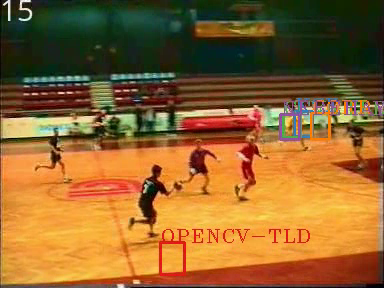
\includegraphics[width=\columnwidth]{handball1-example.png}
		\caption{15. slika posnetka \textit{handball1}.}
		\label{fig:handball1}
	\end{subfigure}
	~
	\begin{subfigure}[t]{0.45\columnwidth}
		\includegraphics[width=\columnwidth]{/handball2-example.png}
		\caption{111. slika posnetka \textit{handball2}.}
		\label{fig:handball2}
	\end{subfigure}  
	\caption[Primer delovanja sledilnikov za \textit{handball} posnetke]{Primer delovanja sledilnikov za \textit{handball} posnetke. Referenčni igralec, ki mu morajo slediti ima rumeno majico. }
	\label{fig:tracker-visual}
\end{figure}




Čeprav smo z mero določili, da se je najbolje izkazal sledilnik CORR, se je pri hitri vizualni oceni sledenja na izsekih posnetka \cite{squashtv2014squash} izkazalo, da najbolje deluje sledilnik KCF. Primer boljšega delovanja KCF sledilnika je slika \ref{fig:squash-tracker-visual}, kjer sledimo modremu igralcu. Na isti sliki posnetka je KCF algoritem našel modrega igralca, medtem ko ga je CORR algoritem zamenjal z drugim igralcem. 



\begin{figure}[!htbp]
	\centering
	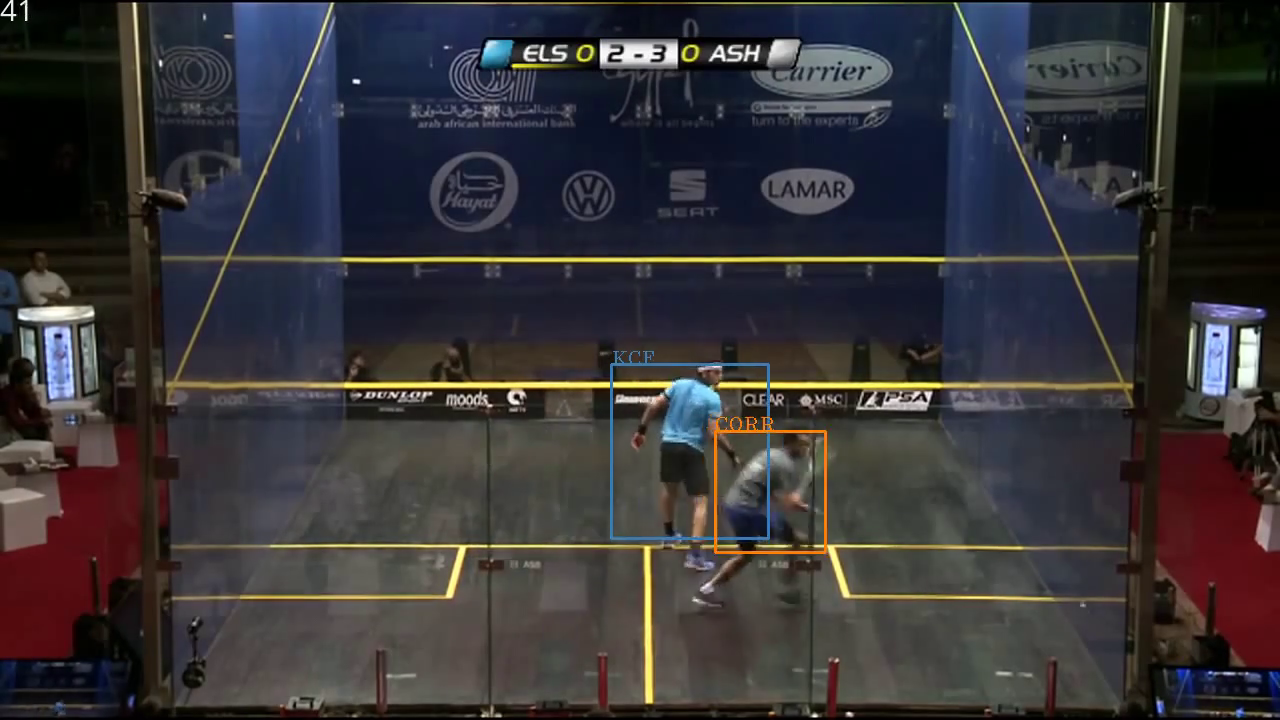
\includegraphics[width=0.6\columnwidth]{preliminary-tracker-squash.png}
	\caption{}
	\caption[Primer delovanja sledilnikov za squash posnetek]{Primer delovanja sledilnikov za squash posnetek. Gre za 41. sliko posnetka \cite{squashtv2014squash}, pri čemer smo uporabili KCF in CORR algoritem. Sledilnika sta morala slediti igralcu z modro majico.}
	\label{fig:squash-tracker-visual}
\end{figure}


Boljše delovanje KCF je razumljivo, saj prvi testi temeljijo na posnetkih rokometa, drugi pa na squashu, kjer gre za bistveno drugačno igro. Če pogledamo tabelo \ref{tab:region-overlap} ima KCF drugo najboljše povprečje, prav tako pa so si rezultati posameznih posnetkov zelo podobni. 


















\subsection{Observabilnost}
Rezultate observabilnosti lahko vidimo v tabeli \ref{tab:observabilnost}. Validacijske metrike so povprečne vrednosti \textit{sv} in \textit{bv} modelov, brez križnega testiranja.  Personov korelacijski koeficient smo povprečili s Fisherjevo $z$ transformacijo. Tako energijska poraba kot srčni utrip, imata visoko pozitivno korelacijo, kar pomeni, da sta oba parametra observabilna. \textit{hr} modeli se po CORR rezultatih bolje ujemajo z referenco, vendar moramo pri tem upoštevati tudi nSV razmerje, ki je tu večje. Če primerjamo metrike napak, \textit{eem} modeli prekašajo \textit{hr} modele. S tem lahko potrdimo, da srčni utrip ni dober fiziološki parameter za določevanje fizične aktivnosti. Najboljši rezultati predikcije energijske porabe in srčnega utripa so prikazani na sliki \ref{fig:stage1-observability}.

\begin{table}[!htbp]
\centering
\begin{tabular}{l S[table-format=1.2, round-mode=places, round-precision=2] S[table-format=1.2, round-mode=places, round-precision=2] S[table-format=1.2, round-mode=places, round-precision=2] S[table-format=1.2, round-mode=places, round-precision=2]}
	\toprule
	\textbf{Model} & \thead{CORR} & \thead{RAE} & \thead{RRSE} & \thead{nSV} \\
		\midrule
		\tdata{observabilnost}
		\bottomrule
		\end{tabular}
		\caption{Validacijske metrike testa observabilnosti. Gre za povprečne vrednosti \textit{sv} in \textit{bv} modelov. Personov korelacijski koeficient (CORR) smo povprečili s Fisherjevo $z$ transformacijo.}
	\label{tab:observabilnost}
	\end{table}
	
\begin{figure}[!htbp]
\centering
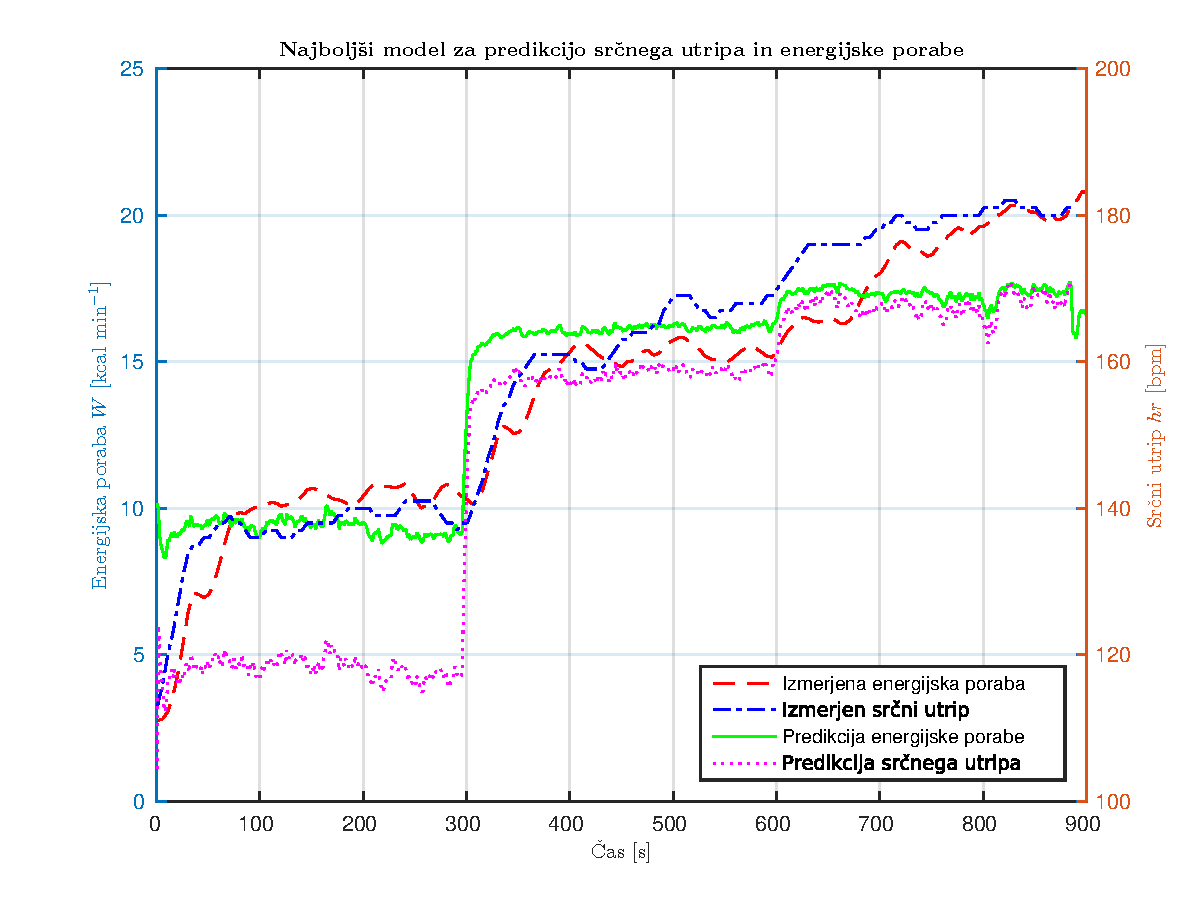
\includegraphics[width=0.5\columnwidth]{best-results-normal--sideview-sideview-normal-sl}
\caption{Najboljši reultati predikcije energijske porabe in srčnega utripa. Slika prikazuje izhode eem-sv(sv) in hr-sv(sv) modelov ter izmerjene vrednosti energijske porabe in srčnega utripa.}
	\label{fig:stage1-observability}
	\end{figure}


\subsection{Ročni izrez}
Tabela \ref{tab:rocni-izrez} prikazuje rezultate ročnega izreza. Prikazani so tudi rezultati observabilnosti za primerjavo. Validacijske metrike so povprečne vrednosti \textit{sv} in \textit{bv} modelov, brez križnega testiranja.  Personov korelacijski koeficient smo povprečili s Fisherjevo $z$ transformacijo. Rezultati modelov z ročnim izrezovanjem so za malenkost slabši. Še vseeno smo jih uporabili v nadaljnih testih, ker se z njimi teoretično znebimo šuma ozadja.

\begin{table}[!htbp]
	\centering
	\begin{tabular}{l S[table-format=1.2, round-mode=places, round-precision=2] S[table-format=1.2, round-mode=places, round-precision=2] S[table-format=1.2, round-mode=places, round-precision=2] S[table-format=1.2, round-mode=places, round-precision=2]}
		\toprule
		\textbf{Model} & \thead{CORR} & \thead{RAE} & \thead{RRSE} & \thead{nSV} \\
		\midrule
		\tdata{rocni-izrez}
		\bottomrule
	\end{tabular}
	\caption{Validacijske metrike testov ročnega izreza. Gre za povprečne vrednosti \textit{sv} in \textit{bv} modelov. Personov korelacijski koeficient (CORR) smo povprečili s Fisherjevo $z$ transformacijo.}
	\label{tab:rocni-izrez}
\end{table}
		
\subsection{Modaliteta}
Rezultati posameznega pogleda kamere so vidni v tabeli \ref{tab:zorni-kot}. Slike smo pred procesiranjem ročno izrezali tako, da smo določili območje tarče, kjer smo zaobjeli celoten subjekt glede na vse sekvence video posnetka. S tem smo simulirali idealni sledilnik. Rezultate tako lažje primerjamo s terenskimi testi.
		
	\begin{table}[!htbp]
	\centering
	\begin{tabular}{l S[table-format=1.2, round-mode=places, round-precision=2] S[table-format=1.2, round-mode=places, round-precision=2] S[table-format=1.2, round-mode=places, round-precision=2] S[table-format=1.2, round-mode=places, round-precision=2]}
\toprule
\textbf{Model} & \thead{CORR} & \thead{RAE} & \thead{RRSE} & \thead{nSV} \\
\midrule
\tdata{zorni-kot}
	\bottomrule
	\end{tabular}
		\caption{Rezultati modalitete zornega kota kamere.}
		\label{tab:zorni-kot}
		\end{table}
		
Če primerjamo \textit{bv(bv)} in \textit{sv(sv)} modele dobimo pri slednjih boljše rezultate. Slabši rezultati hrbtne kamere bi lahko nakazovali na to, da je ta pogled manj informativen. Pri opazovanju križnih testov (testi s podatki različnega pogleda) lahko vidimo, da dobimo pri vseh slabe rezultate. CORR je zelo nizek ali negativen, metrike napak pa so zelo visoke. Glavna razlika mešanih modelov je opazna šele s primerjavo modelov s križnim testiranjem. Rezultati mešanih modelov so veliko boljši in nakazujejo na to, da lahko dobimo boljše rezultate, če uporabimo podatke iz različnih zornih kotov.

Rezultati različne modalitete glede na tip slike so prikazani v tabeli \ref{tab:zorni-kot}. Tudi tu smo posamezne slike sekvenc posnetkov ročno izrezali. V tabeli je prikazana primerjava \textit{ir} in \textit{bv} modelov. \textit{sv} modelov tu ni, saj smo snemali le hrbtne IR posnetke. Rezultati IR posnetkov so boljši, kar se še posebno opazi pri modelih predikcije srčnega utripa.

\begin{table}[!htbp]
\centering
\begin{tabular}{l S[table-format=1.2, round-mode=places, round-precision=2] S[table-format=1.2, round-mode=places, round-precision=2] S[table-format=1.2, round-mode=places, round-precision=2] S[table-format=1.2, round-mode=places, round-precision=2]}
\toprule
\textbf{Model} & \thead{CORR} & \thead{RAE} & \thead{RRSE} & \thead{nSV} \\
\midrule
\tdata{crop-ir}
	\bottomrule
	\end{tabular}
		\caption{Validacijske metrike za različne modalitete glede na tip slike (BGR ali IR).}
		\label{tab:crop-ir}
		\end{table}
	


















\subsection{Modeliranje dodatne zakasnitve}
Modeli z dodatno zakasnitvijo so v tabeli \ref{tab:lag} označeni z \textit{lag}. Opazimo lahko, da so vsi rezultati s zakasnitvijo, ne glede na modaliteto, boljši. Z \textit{lag} modeli smo potrdili predpostavko o zakasnitvi \SI{55}{\s} za energijsko porabo in \SI{15}{\s} za srčni utrip. Ker smo z njimi rešili probleme sinhronizacije, smo jih uporabili v nadaljnih raziskavah. 

\begin{table}[!htbp]
	\centering
	\begin{tabular}{l S[table-format=1.2, round-mode=places, round-precision=2] S[table-format=1.2, round-mode=places, round-precision=2] S[table-format=1.2, round-mode=places, round-precision=2] S[table-format=1.2, round-mode=places, round-precision=2]}
		\toprule
		\textbf{Model} & \thead{CORR} & \thead{RAE} & \thead{RRSE} & \thead{nSV} \\
		\midrule
		\tdata{crop-lag}
		\bottomrule
	\end{tabular}
	\caption{Primerjava rezultatov med modeli z dodatno zakasnitvijo in brez.}
	\label{tab:lag}
\end{table}



\begin{figure}[!htbp]
	\centering
	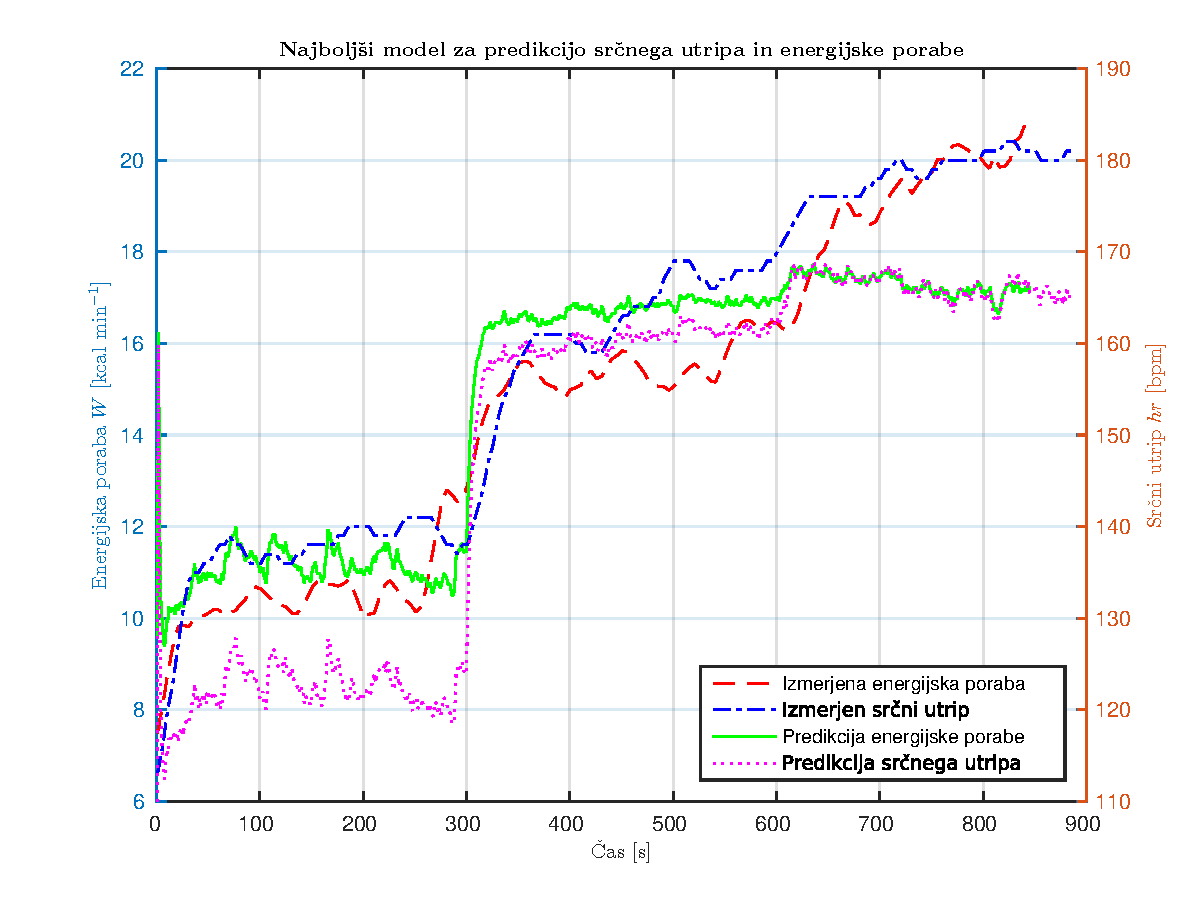
\includegraphics[width=0.5\columnwidth]{best-results-crop-normal-infrared-infrared-lag-sl}
	\caption{Najboljši reultati predikcije energijske porabe in srčnega utripa z upoštevanjem dodatne zakasnitve. Slika prikazuje izhode eem-ir-lag(ir) in hr-ir-lag(ir) modelov ter izmerjene vrednosti energijske porabe in srčnega utripa.}
	\label{fig:crop-lag-rezultat}
\end{figure}

















\subsection{Obremenitveni testi}
Rezultati obremenitvenih testov so prikazani v tabelah \ref{tab:crop-proj} in \ref{tab:crop-scale}. Opazimo lahko, da dobimo pri uporabi IR posnetkov slabše rezultate glede na tabelo \ref{tab:lag}. IR posnetki tako niso primerni za terenske raziskave, saj tam pri snemanju nimamo nikoli idelanih pogojev.

\begin{table}[!htbp]
	\centering
	\begin{tabular}{l S[table-format=1.2, round-mode=places, round-precision=2] S[table-format=1.2, round-mode=places, round-precision=2] S[table-format=1.2, round-mode=places, round-precision=2] S[table-format=1.2, round-mode=places, round-precision=2]}
		\toprule
		\textbf{Model} & \thead{CORR} & \thead{RAE} & \thead{RRSE} & \thead{nSV} \\
		\midrule
		\tdata{crop-proj}
		\bottomrule
	\end{tabular}
	\caption{Validacijske metrike rezultatov s projektivno transformacijo slik posnetkov.}
	\label{tab:crop-proj}
\end{table}

\begin{table}[!htbp]
	\centering
	\begin{tabular}{l S[table-format=1.2, round-mode=places, round-precision=2] S[table-format=1.2, round-mode=places, round-precision=2] S[table-format=1.2, round-mode=places, round-precision=2] S[table-format=1.2, round-mode=places, round-precision=2]}
		\toprule
		\textbf{Model} & \thead{CORR} & \thead{RAE} & \thead{RRSE} & \thead{nSV} \\
		\midrule
		\tdata{crop-sc}
		\bottomrule
	\end{tabular}
	\caption{Rezultati obremenitvenega testa skaliranja.}
	\label{tab:crop-scale}
\end{table}










\subsection{Tekalna steza s sledenjem}
Pri testiranju vpeljve sledilnika smo dobili rezultate v tabeli \ref{tab:shake}. Z vpeljavo sledilnika smo dobili celo nekoliko boljše rezultate od tistih z ročnim izrezovanjem (tabela \ref{tab:lag}). To si lahko razlagamo s tem, da je z uporabo sledilnika določitev območja tarče bolj optimalno, saj je območje določeno za vsako sliko posebej. Zaradi tega so modeli bolj robustni na šum ozadja.

%Results of models with enabled tracker are represented in Table \ref{tab:tracker-models-validation}. If we compare them with results of initial models in Table \ref{tab:initial-models-validation}, the mean absolute difference of RRSE between them is \SI{28}{\%}. We can assume that this is due to the fact that tracker does not track selected object perfectly. In some cases it cannot find object, or detects wrong object. It can also track only part of the object. This anomalies can affect calculation of physiological parameters.



\begin{table}[!htbp]
	\centering
	\begin{tabular}{l S[table-format=1.2, round-mode=places, round-precision=2] S[table-format=1.2, round-mode=places, round-precision=2] S[table-format=1.2, round-mode=places, round-precision=2] S[table-format=1.2, round-mode=places, round-precision=2]}
		\toprule
		\textbf{Model} & \thead{CORR} & \thead{RAE} & \thead{RRSE} & \thead{nSV} \\
		\midrule
		\tdata{shake}
		\bottomrule
	\end{tabular}
	\caption{Tracker normal and tracker shake}
	\label{tab:shake}
\end{table}


Srednja absolutna razlika RRSE metrike med modeli s sledenjem in simulacijo vibracij je okoli \SI{30}{\%}. Rezultati s simulacijo vibracij so slabši, vendar še vedno sprejemljivi, saj sledilnik bolje stabilizira posnetek.











\subsection{Terenski eksperimenti squash igre}
Terenski rezultati squash igre z različnimi deskriptorji so predstavljeni v tabeli \ref{tab:squash}.  Rezultatov ne moremo pravilno evaluirati, ker imamo preobremenjene modele. Zaključimo lahko, da postopek 1. faze ne moremo uporabljati za terenske eksperimente. Odziv preobremenjenih modelov lahko vidimo na sliki \ref{fig:squash-rezultat}.

\begin{table}[!htbp]
	\centering
	\begin{tabular}{l S[table-format=1.2, round-mode=places, round-precision=2] S[table-format=1.2, round-mode=places, round-precision=2] S[table-format=1.2, round-mode=places, round-precision=2] S[table-format=1.2, round-mode=places, round-precision=2]}
		\toprule
		\textbf{Model} & \thead{CORR} & \thead{RAE} & \thead{RRSE} & \thead{nSV} \\
		\midrule
		\tdata{squash-mag}
		\bottomrule
	\end{tabular}
	\caption{Validacijske metrike terenskega testiranja. Tu uporabljamo HOOF in HOOF-HAFA deskriptorje. Modeli so neveljavni.}
	\label{tab:squash}
\end{table}

\begin{figure}[!htbp]
	\centering
	\includegraphics[width=0.5\columnwidth]{best-results-preliminary-squash2-normal-backview-backview-lag-sl}
	\caption{Odziv modela hr-bv-lag-hoofhafa(bv) za squash igro eksperimentov 1. faze.}
	\label{fig:squash-rezultat}
\end{figure}






















\subsection{Eksperiment detekcije dihanja}
Za detekcijo dihanja, ki smo jo formulirali kot problem razrščanja v razrede, smo uporabili standardne metrike za evaluacijo dvorazrednega problema. ``Diha'' smo označili kot pozitivno vrednost, ``ne diha'' pa negativno. Dobili smo sledeče rezultate: Razmerje napačno potrjenih FPR = \SI{13}{\%}, razmerje pravilno potrjenih TPR = \SI{87}{\%}, razmerje napačno zavrnjenih FNR = \SI{26}{\%}, razmerje pravilno zavrnjenih TNR = \SI{74}{\%}. Rezultati so prav tako prikazani s kontigenčno matriko na sliki \ref{fig:breathtest-confusion} in ROC krivuljno \ref{fig:breathtest-roc}.

\begin{figure}[!htbp]
	\centering
	\includegraphics[width=0.5\linewidth]{breathtest-confusion-sl}
	\caption{Kontigenčna matrika med ciljnim in izhodnim razredom za detekcijo dihanja. Razred $1$ pomeni ``diha''. Razred $0$ pomeni ``ne diha''.}
	\label{fig:breathtest-confusion}
\end{figure}

\begin{figure}[!htbp]
	\centering
	\includegraphics[width=0.5\linewidth]{breathtest-roc-sl}
	\caption{ROC krivulja za detekcijo dihanja.}
	\label{fig:breathtest-roc}
\end{figure}




























\section{Eksperimenti 2. faze}
\subsection{Preliminarni eksperimenti}
\subsubsection{Združevanje slik iz dveh Kinect kamer}\label{sec:rezultati-zdruzevanje}
Združevanje s značilkami se ni obneslo, zato smo to metodo opustili. Primer neuspelega poskusa je prikazan na sliki \ref{fig:zdruzevanje-znacilke}.

\begin{figure}[!htb]
	\centering
	\begin{subfigure}[t]{0.45\columnwidth}
		\includegraphics[width=\columnwidth]{./Slike/matched-features.png}
		\caption{Ujemajoče SURF značilke}
		\label{fig:zdruzevanje-surf}
	\end{subfigure}
	~
	\begin{subfigure}[t]{0.45\columnwidth}
		\includegraphics[width=\columnwidth]{./Slike/features-calibration-result.png}
		\caption{Rezultat združevanja z značilkami}
		\label{fig:zdruzevanje-result}
	\end{subfigure}
	\caption{Primer neuspelega poskusa združevanja slik iz dveh Kinect kamer s SURF značilkami.}
	\label{fig:zdruzevanje-znacilke}
\end{figure}

 Rezultat združevanja s kontrolnimi točkami je bil boljši od združevanja z značilkami, vendar še vedno slab, zato smo tudi to metodo opustili. Primer neuspelega poskusa je prikazan na sliki \ref{fig:zdruzevanje-cp}.
 
 \begin{figure}[!htb]
 	\centering
 	\begin{subfigure}[t]{0.45\columnwidth}
 		\includegraphics[width=\columnwidth]{matched-points.png}
 		\caption{Ujemajoče kontrolne točke}
 		\label{fig:zdruzevanje-ujemajoce-cp}
 	\end{subfigure}
 	~
 	\begin{subfigure}[t]{0.45\columnwidth}
 		\includegraphics[width=\columnwidth]{points-calibration-result.png}
 		\caption{Rezultat združevanja s kontrolnimi točkami}
 		\label{fig:zdruzevanje-result-cp}
 	\end{subfigure}
 	\caption{Primer neuspelega poskusa združevanja slik iz dveh Kinect kamer s kontolnimi točkami.}
 	\label{fig:zdruzevanje-cp}
 \end{figure}











\subsubsection{Optimizacija Gaussovega filtra}
Rezultati povrprečnih vrednosti uporabljenih metrik so vidni v tabeli \ref{tab:gauss}. Za pravilno razlago rezultatov, moramo upoštevati tudi grafe metrik posameznih eksperimentov, ki so prikazani na slikah \ref{fig:sigma1-5}, \ref{fig:sigma-rmse5-21} in \ref{fig:sigma21-51}. 



\begin{table}[!htb]
	\centering
	\begin{tabular}{S[table-format=2.0, round-mode=places, round-precision=2] S[table-format=1.2, round-mode=places, round-precision=2] S[table-format=2.2, round-mode=places, round-precision=2]}
		\toprule
		\thead{$\mathbf{\sigma}$} & \thead{RMSE} & \thead{SNR [dB]}  \\
		\midrule
		1 & 4.7764 & 24.1892\\
		3 & 6.3162 & 25.5183\\
		5 & 6.5385 & 25.8459\\
		11 & 6.6457 & 26.1244\\
		21 & 6.6794 & 26.2933\\
		31 & 6.6951 & 26.3922\\
		51 & 6.7155 & 26.5345\\
		\bottomrule
	\end{tabular}
	\caption[Povprečne vrednosti RMSE in SNR metrik pri optimizaciji parametra $\sigma$ Gaussovega filtra]{Povprečne vrednosti RMSE in SNR metrik pri optimizaciji parametra $\sigma$ Gaussovega filtra. Najmanjši standardni odklon ima najmanjšo napako, vendar je tudi filtriranje majhno. Pri $\sigma=3$ in $\sigma=5$ so še opazne razlike pri filriranju. Za višje vrednosti ni več opazne razlike, vendar pa se napaka povečuje. $\sigma=5$ je tako optimalna vrednosti parametra.}
	\label{tab:gauss}
\end{table}

Najmanjšo napako dobimo, če uporabimo $\sigma=1$, vendar pa imamo pri tem najmanjše filtriranje, zato so rezultati še vedno lahko zelo šumni. Z višanjem parametra filtra, se napaka po metriki RMSE povečuje, vendar ima večji vpliv razmerje SNR, saj je predstavljeno v logaritemski skali. 

\begin{figure}[!htb]
	\centering
	\begin{subfigure}[t]{0.45\columnwidth}
		\includegraphics[width=\columnwidth]{sigma-rmse1-5-sl}
		\caption{Graf RMSE  učnih vzorcev }
		\label{fig:sigma-rmse1-5}
	\end{subfigure}
	~
	\begin{subfigure}[t]{0.45\columnwidth}
		\includegraphics[width=\columnwidth]{sigma-snr1-5-sl}
		\caption{Graf SNR  učnih vzorcev}
		\label{fig:sigma-snr1-5}
	\end{subfigure}
	\caption{Grafa RMSE in SNR učnih vzorcev za \mbox{$\sigma \in [1,5]$}}
	\label{fig:sigma1-5}
\end{figure}

Čeprav pri uporabi $\sigma=51$ dobimo največje filtriranje šuma, lahko na slikah grafov opazimo, da se obe metriki bistveno ne razlikujeta za vrednosti parametra na intervalu $[5,51]$. Kljub dobremu filtriranju želimo zagotoviti čim manjšo napako med referenčnim signalom in predikcijo, zato je logična izbira čim manjši standardni odklon. Ker so na sliki \ref{fig:sigma1-5} med $\sigma=3$ in $\sigma=5$ še opazne razlike, lahko zaključimo, da je $\sigma=5$ optimalna izbira parametra za naš problem. 


\begin{figure}[!htb]
	\centering
	\begin{subfigure}[t]{0.45\columnwidth}
		\includegraphics[width=\columnwidth]{sigma-rmse5-21-sl}
		\caption{Graf RMSE  učnih vzorcev}
		\label{fig:sigma-rmse5-21}
	\end{subfigure}
	~
	\begin{subfigure}[t]{0.45\columnwidth}
		\includegraphics[width=\columnwidth]{sigma-snr5-21-sl}
		\caption{Graf SNR  učnih vzorcev}
		\label{fig:sigma-snr5-21}
	\end{subfigure}
	\caption{Grafa RMSE in SNR učnih vzorcev za \mbox{$\sigma \in [5,21]$}}
	\label{fig:sigma5-21}
\end{figure}



\begin{figure}[!htb]
	\centering
	\begin{subfigure}[t]{0.45\columnwidth}
		\includegraphics[width=\columnwidth]{sigma-rmse21-51-sl}
		\caption{Graf RMSE učnih vzorcev}
		\label{fig:sigma-rmse21-51}
	\end{subfigure}
	~
	\begin{subfigure}[t]{0.45\columnwidth}
		\includegraphics[width=\columnwidth]{sigma-snr21-51-sl}
		\caption{Graf SNR  učnih vzorcev}
		\label{fig:sigma-snr21-51}
	\end{subfigure}
	\caption{Grafa RMSE in SNR učnih vzorcev za \mbox{$\sigma \in [21,51]$}}
	\label{fig:sigma21-51}
\end{figure}


\subsubsection{Rezultati mrežnega iskanja \texorpdfstring{$\nu$}{nu}-RBF}
Rezultati optimizacije parametra $\numax$ so predstavljeni v tabeli \ref{tab:nu-max}. Pri validaciji ni opaznih sprememb med različnim parametrom $\numax$ zaradi slabih modelov, zato smo preverili verifikacijo. Pri verifikaciji lahko opazimo, da se s povečevanjem parametra povečuje število podpornih vektorjev, vendar nSV nikoli ne doseže željene vrednosti $\numax$. Kljub podoptimalnosti modelov, z višjimi vrednostmi $\numax$ dobimo boljše rezultate. Razlike med $\numax=0.5$ in $\numax=0.8$ so minimalne zato lahko zaključimo, da potrebujemo za dobro delovanje vsaj $\numax=0.5$. 

\begin{table}[!htbp]
	\centering
	\begin{tabular}{l S[table-format=1.2, round-mode=places, round-precision=2] S[table-format=1.2, round-mode=places, round-precision=2] S[table-format=1.2, round-mode=places, round-precision=2] S[table-format=1.2, round-mode=places, round-precision=2]}
		\toprule
		\textbf{Model} & \thead{CORR} & \thead{RAE} & \thead{RRSE} & \thead{nSV} \\
		\midrule
		\tdata{nu-max}
		\bottomrule
	\end{tabular}
	\caption{Verifikacijske metrike pri optimizaciji parametra $\numax$ postopka mrežnega iskanja \nurbf.}
	\label{tab:nu-max}
\end{table}


Tabela \ref{tab:rbf-nu} predstavlja primerjavo med postopkom z uporabo \nurbf in brez. Metrike so povprečne vrednosti \textit{sv} in \textit{bv} modalitet, pri čemer nismo upoštevali ročnega izrezovanja slik. Pearsonov korelacijski koeficient (CORR) smo povprečili s Fisherjevo $z$ transformacijo. Rezultati nakazujejo, da lahko z uporabo \nurbf dobimo izboljšane rezultate.

\begin{table}[!htbp]
	\centering
	\begin{tabular}{l S[table-format=1.2, round-mode=places, round-precision=2] S[table-format=1.2, round-mode=places, round-precision=2] S[table-format=1.2, round-mode=places, round-precision=2] S[table-format=1.2, round-mode=places, round-precision=2]}
		\toprule
		\textbf{Model} & \thead{CORR} & \thead{RAE} & \thead{RRSE} & \thead{nSV} \\
		\midrule
		\tdata{rbf-nu}
		\bottomrule
	\end{tabular}
	\caption{Validacijske metrike za primerjavlo med postopkom z \nurbf in brez. Gre za povprečne vrednosti \textit{sv} in \textit{bv} modelov. Personov korelacijski koeficient (CORR) smo povprečili s Fisherjevo $z$ transformacijo.}
	\label{tab:rbf-nu}
\end{table}




\begin{comment}
\subsubsection{Jedro GHI}
\begin{table}[!htbp]
	\centering
	\begin{tabular}{l S[table-format=1.2, round-mode=places, round-precision=2] S[table-format=1.2, round-mode=places, round-precision=2] S[table-format=1.2, round-mode=places, round-precision=2] S[table-format=1.2, round-mode=places, round-precision=2]}
		\toprule
		\textbf{Model} & \thead{CORR} & \thead{RAE} & \thead{RRSE} & \thead{nSV} \\
		\midrule
		\bottomrule
	\end{tabular}
	\caption{Ghi vmax800}
	\label{tab:ghi}
\end{table}

\begin{figure}[!htbp]
	\centering
	\caption{Ghi best - eem-sv-lag(sv)}
	\label{fig:ghi}
\end{figure}
\end{comment}


\subsubsection{Normalizacija HAFA deskriptorja}
V tabeli \ref{tab:norm-hafa} dobimo slabe rezultate tako za NORMAL model kot tudi za DIAG model, kjer upoštevamo amplitudni faktor $f_A$. Kljub temu so rezultati z upoštevanjem diagonale boljši, kar nakazuje tudi slika \ref{fig:corr-diag}.

\begin{table}[!htbp]
	\centering
	\begin{tabular}{l S[table-format=1.2, round-mode=places, round-precision=2] S[table-format=1.2, round-mode=places, round-precision=2] S[table-format=1.2, round-mode=places, round-precision=2] S[table-format=1.2, round-mode=places, round-precision=2]}
		\toprule
		\textbf{Model} & \thead{CORR} & \thead{RAE} & \thead{RRSE} & \thead{nSV} \\
		\midrule
		\tdata{diag}
		\bottomrule
	\end{tabular}
	\caption{Evaluacijske metrike pri primerjavi modelov NORMAL in DIAG, kjer upoštevamo amplitudni faktor $f_A$. }
	\label{tab:norm-hafa}
\end{table}

\begin{figure}[!htb]
	\centering
	\begin{subfigure}[t]{0.45\columnwidth}
		\includegraphics[width=\columnwidth]{diag-normal-corr-sl}
		\caption{Korelacija za NORMAL model.}
		\label{fig:corr-diag-normal}
	\end{subfigure}
	~
	\begin{subfigure}[t]{0.45\columnwidth}
		\includegraphics[width=\columnwidth]{diag-diag-corr-sl}
		\caption{Korelacija za DIAG model.}
		\label{fig:corr-diag-diag}
	\end{subfigure}
	\caption[]{Grafa korelacij za NORMAL in DIAG model. Kljub slabim rezultatom obeh modelov, je DIAG model občutno boljši.}
	\label{fig:corr-diag}
\end{figure}


\subsection{Laboratorijski eksperiementi}
\subsubsection{Odvisnost na akumulacijo utrujenosti}
V tabeli \ref{tab:stage2-lab-1-mean} je predstavljeno povprečje validacij merjencev za protokol 1. Personov korelacijski koeficient (CORR) smo povprečili s Fisherjevo $z$ transformacijo. Vsi modeli imajo visoko korelacijo z referenco. Napake so majhne. Opazimo, da dobimo boljše rezultate z uporabo prostorskega toka \textit{it}.

\begin{table}[!htbp]
	\centering
	\begin{tabular}{l S[table-format=1.2, round-mode=places, round-precision=2] S[table-format=1.2, round-mode=places, round-precision=2] S[table-format=1.2, round-mode=places, round-precision=2] S[table-format=1.2, round-mode=places, round-precision=2]}
		\toprule
		\textbf{Model} & \thead{CORR} & \thead{RAE} & \thead{RRSE} & \thead{nSV} \\
		\midrule
		\tdata{stage2-lab-1-mean}
		\bottomrule
	\end{tabular}
	\caption{Povprečje validacij merjencev za protokol 1 druge faze laboratorijskih eksperimentov. Personov korelacijski koeficient (CORR) smo povprečili s Fisherjevo $z$ transformacijo.}
	\label{tab:stage2-lab-1-mean}
\end{table}

V tabeli \ref{tab:stage2-lab-2-mean}  predstavljamo povprečje rezultatov za protokol 2. Personov korelacijski koeficient (CORR) smo povprečili s Fisherjevo $z$ transformacijo. Vsi modeli imajo pričakovano nizko korelacijo in veliko napak.

\begin{table}[!htbp]
	\centering
	\begin{tabular}{l S[table-format=1.2, round-mode=places, round-precision=2] S[table-format=1.2, round-mode=places, round-precision=2] S[table-format=1.2, round-mode=places, round-precision=2] S[table-format=1.2, round-mode=places, round-precision=2]}
		\toprule
		\textbf{Model} & \thead{CORR} & \thead{RAE} & \thead{RRSE} & \thead{nSV} \\
		\midrule
		\tdata{stage2-lab-2-mean}
		\bottomrule
	\end{tabular}
	\caption{Povprečje validacij merjencev za protokol 2 druge faze laboratorijskih eksperimentov. Personov korelacijski koeficient (CORR) smo povprečili s Fisherjevo $z$ transformacijo.}
	\label{tab:stage2-lab-2-mean}
\end{table}

Glede na rezultate v tabelah \ref{tab:stage2-lab-1-mean} in  \ref{tab:stage2-lab-2-mean} se utrujenost akumulira skozi čas, kar moramo upoštevati pri gradnji modelov.


\subsubsection{Generalizacija modela}
S protokolom 3 smo želeli preveriti, če lahko uporabimo generaliziran model za predikcijo energijske porabe na različnih merjencih. Rezultati so vidni v tabeli \ref{tab:stage2-lab-3}. Zanimivo dobimo najboljše rezultate za optični tok in ne za prostorskega, kot smo predlagali. Korelacije modelov z optičnim tokom \textit{of} se bližajo vrednosti $1$, vendar pa so metrike napak slabše. Nakazujejo na to, da modeli le niso tako zelo dobri. Vsekakor imamo podobne rezultate tako za SUBJ8 kot za SUBJ9, kar naznanja dobro generalizacijo modela.

\begin{table}[!htbp]
	\centering
	\begin{tabular}{l S[table-format=1.2, round-mode=places, round-precision=2] S[table-format=1.2, round-mode=places, round-precision=2] S[table-format=1.2, round-mode=places, round-precision=2] S[table-format=1.2, round-mode=places, round-precision=2]}
		\toprule
		\textbf{Model} & \thead{CORR} & \thead{RAE} & \thead{RRSE} & \thead{nSV} \\
		\midrule
		%\tdata{stage2-lab-3}
		\bottomrule
	\end{tabular}
	\caption{Validacijske metrike za protokol 3 druge faze laboratorijskih eksperimentov.}
	\label{tab:stage2-lab-3}
\end{table}

Najboljši rezultati za optični in prostoski tok, so predstavljeni na sliki \ref{fig:lab-3}. Odzivi modelov vsebujejo veliko šuma, zato bi lahko uporabili širše Gaussovo jedro za filtriranje rezultatov. Najslabšo predikcijo dobimo za največjo fizično aktivnost.

\begin{figure}[!htbp]
	\centering
	\begin{subfigure}[t]{0.45\columnwidth}
		%\includegraphics[width=\columnwidth]{best-results-stage3-lab-of-3-subj6-sideview-sideview-normal-sl}
		\caption{Rezultati eem-sv-of-subj9(sv) z optičnim tokom}
		\label{fig:lab-of-3}
	\end{subfigure}
	~
	\begin{subfigure}[t]{0.45\columnwidth}
		%\includegraphics[width=\columnwidth]{best-results-stage3-lab-sf-3-subj6-sideview-sideview-normal-sl}
		\caption{Rezultati eem-sv-sf-subj9(sv) s prostorskim tokom}
		\label{fig:lab-sf-3}
	\end{subfigure}
	\caption[Odziv SUBJ9 modelov protokola 3 druge faze laboratorijskih eksperimentov]{Odziv najboljših modelov protokola 3 druge faze laboratorijskih eksperimentov. Rdeča krivulja predstavlja merjen parameter, zelena predikcijo. Na sliki \subref{fig:lab-of-3}) je najboljši rezultat pri uporabi optičnega toka. Na sliki \subref{fig:lab-sf-3}) je najboljši rezultat pri uporabi prostorskega toka.}
	\label{fig:lab-3}
\end{figure}

\subsection{Terenski eksperimenti}
\subsubsection{Odvisnost na akumulacijo utrujenosti}
V tabeli \ref{tab:stage2-field-1-mean} je predstavljeno povprečje validacij merjencev za protokol 1. Personov korelacijski koeficient (CORR) smo povprečili s Fisherjevo $z$ transformacijo. Najboljše rezultate dobimo za prostorski tok \textit{sf}. Korelacija je dokaj visoka, ampak metrike napak nakazujejo na slabši model.

\begin{table}[!htbp]
	\centering
	\begin{tabular}{l S[table-format=1.2, round-mode=places, round-precision=2] S[table-format=1.2, round-mode=places, round-precision=2] S[table-format=1.2, round-mode=places, round-precision=2] S[table-format=1.2, round-mode=places, round-precision=2]}
		\toprule
		\textbf{Model} & \thead{CORR} & \thead{RAE} & \thead{RRSE} & \thead{nSV} \\
		\midrule
		\tdata{stage2-field-1-mean}
		\bottomrule
	\end{tabular}
	\caption{Povprečje validacij merjencev za protokol 1 druge faze terenskih eksperimentov. Personov korelacijski koeficient (CORR) smo povprečili s Fisherjevo $z$ transformacijo.}
	\label{tab:stage2-field-1-mean}
\end{table}

V tabeli \ref{tab:stage2-field-2-mean} predstavljamo povprečje rezultatov za protokol 2. Personov korelacijski koeficient (CORR) smo povprečili s Fisherjevo $z$ transformacijo. Vsi modeli imajo pričakovano nizko korelacijo in veliko napak.

\begin{table}[!htbp]
	\centering
	\begin{tabular}{l S[table-format=1.2, round-mode=places, round-precision=2] S[table-format=1.2, round-mode=places, round-precision=2] S[table-format=1.2, round-mode=places, round-precision=2] S[table-format=1.2, round-mode=places, round-precision=2]}
		\toprule
		\textbf{Model} & \thead{CORR} & \thead{RAE} & \thead{RRSE} & \thead{nSV} \\
		\midrule
		\tdata{stage2-field-2-mean}
		\bottomrule
	\end{tabular}
	\caption{Povprečje validacij merjencev za protokol 2 druge faze terenskih eksperimentov. Personov korelacijski koeficient (CORR) smo povprečili s Fisherjevo $z$ transformacijo.}
	\label{tab:stage2-field-2-mean}
\end{table}

\subsubsection{Generalizacija modela}
S protokolom 3 smo želeli preveriti, če lahko uporabimo generaliziran model za predikcijo energijske porabe na različnih merjencih. Rezultati so vidni v tabeli \ref{tab:stage2-field-3}. Tukaj dobimo najboljše rezultate pri uporabi prostorskega toka, kot smo to predlagali tudi sami. Tudi rezultati optičnega toka niso slabi. Najboljši rezultati za optični in prostoski tok, so predstavljeni na sliki \ref{fig:lab-3}.

\begin{table}[!htbp]
	\centering
	\begin{tabular}{l S[table-format=1.2, round-mode=places, round-precision=2] S[table-format=1.2, round-mode=places, round-precision=2] S[table-format=1.2, round-mode=places, round-precision=2] S[table-format=1.2, round-mode=places, round-precision=2]}
		\toprule
		\textbf{Model} & \thead{CORR} & \thead{RAE} & \thead{RRSE} & \thead{nSV} \\
		\midrule
		\tdata{stage2-field-3}
		\bottomrule
	\end{tabular}
	\caption{Validacijske metrike za protokol 3 druge faze terenskih eksperimentov.}
	\label{tab:stage2-field-3}
\end{table}

\begin{figure}[!htbp]
	\centering
	\begin{subfigure}[t]{0.45\columnwidth}
		\includegraphics[width=\columnwidth]{best-results-stage3-final-field-of-3-subj6-backview-backview-normal-val-sl}
		\caption{Rezultati eem-bv-of-subj9(bf) z optičnim tokom}
		\label{fig:field-of-3}
	\end{subfigure}
	~
	\begin{subfigure}[t]{0.45\columnwidth}
		\includegraphics[width=\columnwidth]{best-results-stage3-final-field-sf-3-subj6-backview-backview-normal-val-sl}
		\caption{Rezultati flow eem-bv-sf-subj9(bv) s prostorskim tokom}
		\label{fig:field-sf-3}
	\end{subfigure}
	\caption[Odziv SUBJ9 modelov protokola 3 druge faze laboratorijskih eksperimentov]{Odziv najboljših modelov protokola 3 druge faze laboratorijskih eksperimentov. Rdeča krivulja predstavlja merjen parameter, zelena predikcijo. Na sliki \subref{fig:field-of-3}) je najboljši rezultat pri uporabi optičnega toka. Na sliki \subref{fig:field-sf-3}) je najboljši rezultat pri uporabi prostorskega toka.}
	\label{fig:field-3}
\end{figure}










